\documentclass[12pt,letterpaper,reqno]{article}

% \usepackage{mathtools}
\usepackage{epsfig}
\usepackage{amsmath}
\usepackage{amssymb}
\usepackage{amsthm}
\usepackage{indentfirst}
\usepackage{xspace}
\usepackage{multirow}
\usepackage{hyperref}
\usepackage{xcolor}
\usepackage{verbatim}
\usepackage[letterpaper,margin=1in,headheight=15pt]{geometry}
\usepackage{mathpazo}
\usepackage{tikz-cd}
\usepackage{booktabs}
\usepackage{framed}
\usepackage{float}
\usepackage{thmtools}
\usepackage{dashrule}
\usepackage[missing=]{gitinfo2}
\usepackage{fancyhdr}
\usepackage{enumerate}
\usepackage{graphicx}
\usepackage{mathrsfs}
\usepackage{calligra}
\usepackage[titletoc,title]{appendix}
\usepackage{caption}
\usepackage{subcaption}

\definecolor{darkblue}{rgb}{0.1,0.1,0.7}
\definecolor{darkred}{rgb}{0.5,0.1,0.1}
\definecolor{darkgreen}{rgb}{0.0,0.42,0.06}
\hypersetup{colorlinks=true,urlcolor=darkred,linkcolor=darkblue,citecolor=darkred}
\definecolor{shadecolor}{rgb}{0.85,0.85,0.85}

% Bibliography formatting
\usepackage[bibstyle=authoryear-comp,labeldate=false,defernumbers=true,maxnames=20,uniquename=init,dashed=false,backend=biber,sorting=none]{biblatex}

\DeclareNameAlias{sortname}{first-last}

\DeclareFieldFormat{url}{\url{#1}}
\DeclareFieldFormat[article]{pages}{#1}
\DeclareFieldFormat[inproceedings]{pages}{\lowercase{pp.}#1}
\DeclareFieldFormat[incollection]{pages}{\lowercase{pp.}#1}
\DeclareFieldFormat[article]{volume}{\textbf{#1}}
\DeclareFieldFormat[article]{number}{(#1)}
\DeclareFieldFormat[article]{title}{\MakeCapital{#1}}
\DeclareFieldFormat[inproceedings]{title}{#1}
\DeclareFieldFormat{shorthandwidth}{#1}

% Don't use "In:" in bibliography. Omit urls from journal articles.
\DeclareBibliographyDriver{article}{%
  \usebibmacro{bibindex}%
  \usebibmacro{begentry}%
  \usebibmacro{author/editor}%
  \setunit{\labelnamepunct}\newblock
  \MakeSentenceCase{\usebibmacro{title}}%
  \newunit
  \printlist{language}%
  \newunit\newblock
  \usebibmacro{byauthor}%
  \newunit\newblock
  \usebibmacro{byeditor+others}%
  \newunit\newblock
  \printfield{version}%
  \newunit\newblock
%  \usebibmacro{in:}%
  \usebibmacro{journal+issuetitle}%
  \newunit\newblock
  \printfield{note}%
  \setunit{\bibpagespunct}%
  \printfield{pages}
  \newunit\newblock
  \usebibmacro{eprint}
  \newunit\newblock
  \printfield{addendum}%
  \newunit\newblock
  \usebibmacro{pageref}%
  \usebibmacro{finentry}}

% Remove dot between volume and number in journal articles.
\renewbibmacro*{journal+issuetitle}{%
  \usebibmacro{journal}%
  \setunit*{\addspace}%
  \iffieldundef{series}
    {}
    {\newunit
     \printfield{series}%
     \setunit{\addspace}}%
  \printfield{volume}%
%  \setunit*{\adddot}%
  \printfield{number}%
  \setunit{\addcomma\space}%
  \printfield{eid}%
  \setunit{\addspace}%
  \usebibmacro{issue+date}%
  \newunit\newblock
  \usebibmacro{issue}%
  \newunit}


% Bibliography categories
\def\makebibcategory#1#2{\DeclareBibliographyCategory{#1}\defbibheading{#1}{\section*{#2}}}
\makebibcategory{books}{Books}
\makebibcategory{papers}{Refereed research papers}
\makebibcategory{chapters}{Book chapters}
\makebibcategory{conferences}{Papers in conference proceedings}
\makebibcategory{techreports}{Unpublished working papers}
\makebibcategory{bookreviews}{Book reviews}
\makebibcategory{editorials}{Editorials}
\makebibcategory{phd}{PhD thesis}
\makebibcategory{subpapers}{Submitted papers}
\makebibcategory{curpapers}{Current projects}

\setlength{\bibitemsep}{2.65pt}
\setlength{\bibhang}{.8cm}
\renewcommand{\bibfont}{\small}

\renewcommand*{\bibitem}{\addtocounter{papers}{1}\item \mbox{}\hskip-0.85cm\hbox to 0.85cm{\hfill\arabic{papers}.~~}}
\defbibenvironment{bibliography}
{\list{}
  {\setlength{\leftmargin}{\bibhang}%
   \setlength{\itemsep}{\bibitemsep}%
   \setlength{\parsep}{\bibparsep}}}
{\endlist}
{\bibitem}

\newenvironment{publications}{\section{\LARGE Publications}\label{papersstart}\vspace*{0.2cm}\small
\titlespacing{\section}{0pt}{1.5ex}{1ex}\itemsep=0.00cm
}{\label{papersend}\addtocounter{sumpapers}{-1}\refstepcounter{sumpapers}\label{sumpapers}}

\def\printbib#1{\printbibliography[category=#1,heading=#1]\lastref{sumpapers}}

% Counters for keeping track of papers
\newcounter{papers}\setcounter{papers}{0}
\newcounter{sumpapers}\setcounter{sumpapers}{0}
\def\lastref#1{\addtocounter{#1}{\value{papers}}\setcounter{papers}{0}}

% theorem environments
\declaretheoremstyle[spaceabove=0.25cm,spacebelow=0.25cm,notefont=\normalfont\bfseries, notebraces={(}{)}]{theorem}
\declaretheoremstyle[spaceabove=0.25cm,spacebelow=0.25cm,bodyfont=\normalfont,notefont=\normalfont\bfseries, notebraces={(}{)}]{noital}
\declaretheoremstyle[spaceabove=0.25cm,spacebelow=0.25cm,bodyfont=\normalfont\color{darkgreen},notefont=\normalfont\bfseries, notebraces={(}{)}]{green}
\declaretheoremstyle[spaceabove=0.25cm,spacebelow=0.25cm,bodyfont=\normalfont,notefont=\normalfont\bfseries,qed=$\qedsymbol$,notebraces={(}{)}]{proofstyle}

\declaretheorem[name=Theorem,numberwithin=section,style=theorem]{thm}
\declaretheorem[name=Proposition,sibling=thm,style=theorem]{prop}
\declaretheorem[name=Corollary,sibling=thm,style=theorem]{cor}
\declaretheorem[name=Lemma,sibling=thm,style=theorem]{lem}
\declaretheorem[name=Definition,sibling=thm,style=noital]{defn}
\declaretheorem[name=Example,sibling=thm,style=noital]{example}
\declaretheorem[name=Exercise,numberwithin=section,style=green]{exercise}
\declaretheorem[name=Proof,style=proofstyle,numbered=no]{pf}
\declaretheorem[name=Solution,style=proofstyle,numbered=no]{solution}
\declaretheorem[name=Remark,style=proofstyle,numbered=no]{remark}
\declaretheorem[name=Remarks,style=proofstyle,numbered=no]{remarks}
\numberwithin{equation}{section}


% macros for convenience
\newcommand{\tops}{\texorpdfstring}

\newcommand{\nid}{\noindent}

\newcommand{\fa}{{\mathfrak a}}
\newcommand{\fp}{{\mathfrak p}}
\newcommand{\fk}{{\mathfrak k}}
\newcommand{\fg}{{\mathfrak g}}
\newcommand{\fh}{{\mathfrak h}}
\newcommand{\fn}{{\mathfrak n}}
\newcommand{\fq}{{\mathfrak q}}
\newcommand{\fm}{{\mathfrak m}}
\newcommand{\fr}{{\mathfrak r}}
\newcommand{\fu}{{\mathfrak u}}
\newcommand{\fG}{{\mathfrak G}}
\newcommand{\bh}{{\bf h}}

\newcommand{\cC}{\ensuremath{\mathcal C}}
\newcommand{\cG}{\ensuremath{\mathcal G}}
\newcommand{\cB}{\ensuremath{\mathcal B}}
\newcommand{\cL}{\ensuremath{\mathcal L}}
\newcommand{\cS}{\ensuremath{\mathcal S}}
\newcommand{\cF}{\ensuremath{\mathcal F}}
\newcommand{\cK}{\ensuremath{\mathcal K}}
\newcommand{\cZ}{\ensuremath{\mathcal Z}}
\newcommand{\cM}{\ensuremath{\mathcal M}}
\newcommand{\cN}{\ensuremath{\mathcal N}}
\newcommand{\cO}{\ensuremath{\mathcal O}}
\newcommand{\cH}{\ensuremath{\mathcal H}}
\newcommand{\cX}{\ensuremath{\mathcal X}}
\newcommand{\cY}{\ensuremath{\mathcal Y}}
\newcommand{\cA}{\ensuremath{\mathcal A}}
\newcommand{\cI}{\ensuremath{\mathcal I}}

\newcommand{\R}{\ensuremath{\mathbb R}}
\newcommand{\C}{\ensuremath{\mathbb C}}
\newcommand{\PP}{\ensuremath{\mathbb P}}
\newcommand{\Z}{\ensuremath{\mathbb Z}}
\newcommand{\Q}{\ensuremath{\mathbb Q}}
\newcommand{\A}{\ensuremath{\mathbb A}}
\newcommand{\bbH}{\ensuremath{\mathbb H}}
\newcommand{\bbI}{\ensuremath{\mathbb I}}
\newcommand{\bS}{\ensuremath{\mathbb S}}

\newcommand{\half}{\ensuremath{\frac{1}{2}}}
\newcommand{\qtr}{\ensuremath{\frac{1}{4}}}
\newcommand{\bq}{{\mathbf q}}
\newcommand{\N}{{\mathbb N}}
\newcommand{\F}{{\mathcal F}}
\newcommand{\HH}{{\mathcal H}}
\newcommand{\LL}{{\mathcal L}}
\newcommand{\RR}{{\mathcal R}}
\newcommand{\V}{{\mathcal V}}
\newcommand{\dirac}{\!\!\not\!\partial}
\newcommand{\Dirac}{\!\!\not\!\!D}
\newcommand{\cE}{{\mathcal E}}
\newcommand{\vs}{\not\!v}
\newcommand{\kahler}{K\"ahler\xspace}
\newcommand{\kq}{/\!\!/}
\newcommand{\kql}[1]{/\!\!/\!\!_#1\,}
\newcommand{\hk}{hyperk\"ahler\xspace}
\newcommand{\Hk}{Hyperk\"ahler\xspace}
\newcommand{\hkq}{/\!\!/\!\!/\!\!/}
\newcommand{\hkql}[1]{/\!\!/\!\!/\!\!/\!\!_#1\,}
\newcommand{\del}{\ensuremath{\partial}}
\newcommand{\delbar}{\ensuremath{\overline{\partial}}}
\newcommand{\bl}{{\bf L}}
\newcommand{\J}{{\mathrm j}}
\newcommand{\K}{{\mathrm k}}
\newcommand{\e}{{\mathrm e}}
\newcommand\bid{{\mathbf 1}}
\newcommand{\de}{\mathrm{d}}
\newcommand{\ab}{\mathrm{ab}}
\newcommand{\vol}{\mathrm{vol}}
\renewcommand{\sf}{\mathrm{sf}}
\newcommand{\inst}{\mathrm{inst}}
\newcommand{\eff}{\mathrm{eff}}
\newcommand{\dR}{\mathrm{dR}}
\newcommand{\closed}{\mathrm{closed}}
\newcommand{\exact}{\mathrm{exact}}
\newcommand{\zv}{{\bf 0}}
\newcommand{\bbf}{{\bf F}}

\newcommand{\abs}[1]{\lvert#1\rvert}
\newcommand{\norm}[1]{\lVert#1\rVert}
\newcommand{\IP}[1]{\langle#1\rangle}
\newcommand{\DIP}[1]{\langle\!\langle#1\rangle\!\rangle}
\newcommand{\dwrt}[1]{\frac{\partial}{\partial#1}}
\newcommand{\eps}{\epsilon}
\newcommand{\simarrow}{\xrightarrow\sim}

\newcommand{\mmaref}[1]{}

\newcommand{\ti}[1]{\textit{#1}}
\newcommand{\tb}[1]{\textbf{#1}}
\newcommand{\lo}{\text{\calligra o}\,}
\newcommand{\dd}{\ensuremath{\mathscr{D}}}
\newcommand{\bu}{{\bf u}}
\newcommand{\bv}{{\bf v}}
\newcommand{\bw}{{\bf w}}
\newcommand{\bx}{{\bf x}}
\newcommand{\by}{{\bf y}}
\newcommand{\bz}{{\bf z}}
\newcommand{\ba}{{\bf a}}
\newcommand{\bb}{{\bf b}}
\newcommand{\bbr}{{\bf r}}
\newcommand{\bff}{{\bf f}}
\newcommand{\bgg}{{\bf g}}
\newcommand{\bt}{{\bf t}}
\newcommand{\bn}{{\bf n}}
\newcommand{\ii}{{\bf {\hat{i}}}}
\newcommand{\jj}{{\bf {\hat{j}}}}
\newcommand{\kk}{{\bf {\hat{k}}}}
\newcommand{\ut}{{\bf {\hat{t}}}}
\newcommand{\un}{{\bf {\hat{n}}}}
\newcommand{\ub}{{\bf {\hat{b}}}}
\newcommand{\bj}{{\bf j}}


\DeclareMathOperator{\ad}{ad}
\DeclareMathOperator{\im}{Im}
\DeclareMathOperator{\re}{Re}
\DeclareMathOperator{\Tr}{Tr}
\DeclareMathOperator{\End}{End}
\DeclareMathOperator{\Hom}{Hom}
\DeclareMathOperator{\Aut}{Aut}
\DeclareMathOperator{\Sym}{Sym}
\DeclareMathOperator{\Lie}{Lie}
\DeclareMathOperator{\diag}{diag}
\DeclareMathOperator{\Bun}{Bun}
\DeclareMathOperator{\Vect}{Vect}
\DeclareMathOperator{\Span}{Span}
\DeclareMathOperator{\grad}{grad}
\DeclareMathOperator{\rank}{rank}
\DeclareMathOperator{\ind}{ind}
\DeclareMathOperator{\coker}{coker}
\DeclareMathOperator{\Jac}{Jac}
\DeclareMathOperator{\Hol}{Hol}
\DeclareMathOperator{\gr}{gr}

\newcommand{\insfig}[2]{

\medskip
\noindent
\begin{minipage}{\linewidth}

\makebox[\linewidth]{\includegraphics[keepaspectratio=true,scale=#2]{figures/#1-crop.pdf}}

\end{minipage}
\medskip

}


% \newcommand{\insfig}[2]{\begin{figure}[htbp] \centering \includegraphics[scale=#2]{figures/#1-crop.pdf} \label{fig:#1} \end{figure}}
% syntax: \insfig{name}{0.5}{caption}

\newcommand{\fixme}[1]{{\color{orange}{[#1]}}}
\newcommand{\currentposition}{{\color{blue} \noindent\makebox[\linewidth]{\hdashrule{\paperwidth}{1pt}{3mm}}}}

% \mathtoolsset{showonlyrefs}

\bibliography{mvc}

\begin{document}
\pagestyle{fancy}
\lhead{{\tiny \color{gray} \tt \gitAuthorIsoDate}}
\chead{\tiny \ti{Multivariable Calculus, GSMST Spring 2020}}
\rhead{{\tiny \color{gray} \tt \gitAbbrevHash}}
\renewcommand{\headrulewidth}{0.5pt}


\begin{center}
\tb{Multivariable Calculus \\
Semester 2: Multivariable Calculus} \\
Anderson Trimm \\
Gwinnett School of Mathematics, Science and Technology \\
\end{center}

{These are the notes for the Spring Semester 2020
course in Multivariable Calculus at GSMST. They will continually be updated throughout the course. The latest PDF can always be accessed
at \small \url{https://github.com/atrimm/mvc/blob/master/Course%20Notes/multivariable_calculus_2020.pdf.}

\tableofcontents
\renewcommand{\listtheoremname}{Quick reference}
\listoftheorems[onlynamed]

\newpage

%\setcounter{page}{1}

\section{Curves}
In this section we study functions with one input and multiple outputs.

\subsection{Vector-valued functions}
\subsubsection{Definitions}
Suppose a particle moves in the plane along the following curve $C$:
	\begin{figure}[h]
		\begin{center}
		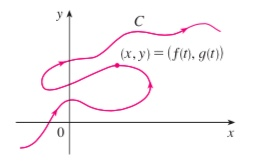
\includegraphics[scale=0.5]{figures_mvc/plane_curve}
	\end{center}
	\caption{Trajectory of a particle moving in the plane.}
	\end{figure}
Since the curve fails the vertical line test, $C$ cannot be described as the graph of a function $y=f(x)$. Note however that the x- and y-coords of the particle are functions of time
\begin{align*}
	x=f(t), \hspace{0.5cm} y=g(t)
\end{align*}
so the curve $C$ can be described as the image of function ${\bf r}:I \to \mathbb{R}^2$ defined by 
\begin{align*}
	\bbr(t)=(f(t),g(t)),
\end{align*}
where $I=[a,b]$ is an interval in $\R$. 
\begin{figure}[h]
	\begin{center}
		\includegraphics[scale=0.3]{figures_mvc/mapping_diag}
	\end{center}
	\caption{A mapping diagram showing the function $\bbr:I \to \R^2$.}
\end{figure}

\begin{defn}[Vector-valued function]
Let $I \subseteq \R$. A mapping $\bbr:I \to \mathbb{R}^n$ called a \emph{vector-valued function}. The value of $\bbr$ at $t \in I$ can be written as
\begin{align*}
	\bbr(t)=(r_1(t),r_2(t),\dots,r_n(t))
\end{align*}
where the $n$ functions $r_i:I \to \R$, $i=1,\dots,n$ are called the \emph{component functions} of $\bbr$.	
\end{defn}
Unless specified otherwise, we will take the domain $I$ of a vector-valued function to be the largest domain on which all of the component functions are defined.
\begin{example}
Consider the vector-valued function $\bbr:I \to \mathbb{R}^3$ defined by
	\begin{align*}
		\bbr(t)=(t^3,\ln(3-t),\sqrt{t}).
	\end{align*}
The component functions of $\bbr(t)$ are 
\begin{align*}
	r_1(t)=t^3, \hspace{0.5cm} r_2(t)=\ln(3-t), \hspace{0.5cm} r_3(t)=\sqrt{t}.
\end{align*}
The domains of each of these functions, respectively, are 
\begin{align*}
	I_1=\R, \hspace{0.5cm} I_2=(-\infty,3), \hspace{0.5cm} I_3=[0,\infty),
\end{align*}	
so the domain $I$ of $\bbr(t)$ is 
\begin{align*}
	I=I_1 \cap I_2 \cap I_3=[0,3).
\end{align*} 
\end{example}
This function can be visualized in \emph{Mathematica} using``ParametricPlot3D":

\begin{figure}[h]
	\begin{center}
		\includegraphics[scale=0.5]{figures_mvc/vv_fcn_first-ex}
	\end{center}
	\caption{Plot of the vector-valued function $\bbr(t)=(t^3,\ln(3-t),\sqrt{t})$ from $t=0$ to $t=1$.}
\end{figure}

\begin{exercise}
	Consider the vector-valued function $\bbr:I \to \mathbb{R}^3$ defined by
	\begin{align*}
		\bbr(t)=\left(\frac{t-2}{t+2},\sin t, \ln(9-t^2)\right).
	\end{align*}
What is the domain $I$ of the function?
\end{exercise}
{\color{red}\begin{solution}
	The component functions of $\bbr(t)$ are 
	\begin{align*}
		r_1=\frac{t-2}{t+2}, \hspace{0.5cm} r_2=\sin t, \hspace{0.5cm} r_3=\ln(9-t^2).
	\end{align*}
	The domains of $r_1(t)$ and $r_2(t)$ are given, respectively, by
	\begin{align*}
		I_1=(-\infty,-2) \cup (-2,\infty), \hspace{0.5cm} I_2=\R.
	\end{align*}
	To find the domain of $r_3(t)$, we need to solve the inequality
	\begin{align*}
		9-t^2>0. \\
	\end{align*}
	The graph of the function $y=9-x^2$ is a concave-down parabola with $y$-intercept 9 and $x$-intercepts $\pm 3$. 
	
	\begin{figure}[h]
	\begin{center}
		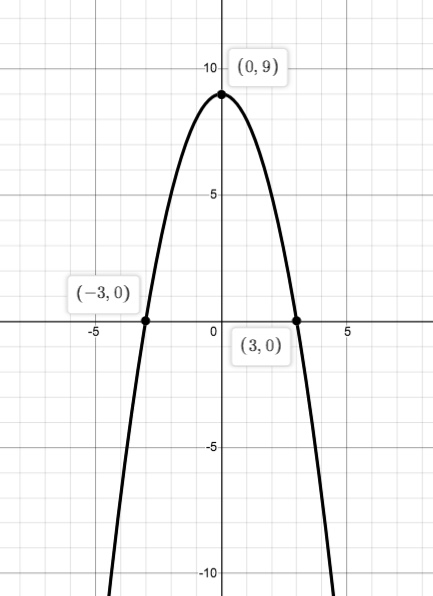
\includegraphics[scale=0.3]{figures_mvc/parab_down}
	\end{center}
	\caption{Graph of $y=9-x^2$.}
\end{figure}
	We have $y>0$ where the graph is above the $x$-axis, so $y>0$ when $-3<x<3$. The domain of $r_3(t)$ is therefore
	\begin{align*}
		I_3=(-3,3).
	\end{align*}
	The domain of $\bbr(t)$ is then
	\begin{align*}
		I=I_1 \cap I_2 \cap I_3=(-3,-2)\cup (-2,3).
	\end{align*}
\end{solution}}

\subsubsection{Review: limits of single-variable functions}
Before considering limits of vector-valued functions, let's review the definition for a real-valued function $y=f(x)$ of a single real variable $x$.

To motivate the definition, consider the function
\begin{align*}
	f(x)=\begin{cases}
		2x-1, \ \text{ if } x \neq 3 \\
		6, \hspace{1.0cm} \text{ if } x = 3 \\
	\end{cases}
\end{align*}
whose graph is shown in the figure below.

\begin{figure}[h]\label{fig:lim_def}
	\begin{center}
		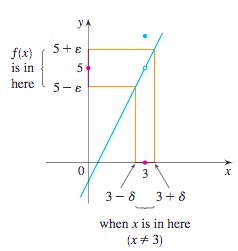
\includegraphics[scale=0.7]{figures_mvc/graph_limit_defn}
	\end{center}
	\caption{Graph of the function $y=f(x)$ in the example above.}
\end{figure}
From the graph, we see that when $x$ is close to 3 but not equal to 3, then $f(x)$ is close to 5, and so $\lim_{x \to 3}f(x)=5$.

However, it is important to be able to state this precisely. For instance, we may ask: \emph{How close to 3 does $x$ have to be so that $f(x)$ differs from 5 by less than $0.1$?}

The distance from $x$ to $3$ is $|x-3|$ and the distance from $f(x)$ to 5 is $|f(x)-5|$, so our problem is to find a number $\delta$ such that 
\begin{align*}
	|f(x)-5|<0.1 \hspace{0.5cm} \text{ if } \hspace{0.5cm} 0<|x-3|<\delta.
\end{align*}
If $x \neq 3$, then 
\begin{align*}
	|f(x)-5|=|(2x-1)-5|=|2x-6|=2|x-3|
\end{align*}
so we see that by taking $\delta=\frac{1}{2}(0.1)=0.05$, we have $|f(x)-5|<2(0.05)=0.1$. Thus, an answer to the problem is given by $\delta=0.05$; that is, if $x$ is within a distance of $0.05$ from 3, then $f(x)$ will be within a distance of $0.1$ from 5.

If we change the number $0.1$ in our problem to the smaller number $0.01$, then by using the same method we find that $f(x)$ will differ from 5 by less than $0.01$ provided that $x$ differs from 3 by less than $\frac{1}{2}(0.01)=0.005$; that is,
\begin{align*}
	|f(x)-5|<0.01 \hspace{0.5cm} \text{ if } \hspace{0.5cm} 0<|x-3|<0.005.
\end{align*}
Similarly,
\begin{align*}
	|f(x)-5|<0.001 \hspace{0.5cm} \text{ if } \hspace{0.5cm} 0<|x-3|<0.0005.
\end{align*}
Think of the numbers $0.1, 0.01, 0.001$ above as \emph{error tolerances} that we might allow. That is, when challenged with an error tolerance, it is our task to find a corresponding $\delta$ so that whenever $x$ is within a distance of $\delta$ from 3, $f(x)\approx 5$, within the given error tolerance. 

Now for 5 to be the precise limit of $f(x)$ as $x$ approaches 3, we must not only be able to bring the difference between $f(x)$ and 5 below each of these numbers; we must be able to bring it below \emph{any} positive number. And, by exactly the same reasoning, we can. That is, if $\epsilon$ is any positive number, then by choosing $\delta=\frac{\epsilon
}{2}$, we find
\begin{align}\label{eq:review_limit_example}
	|f(x)-5|<\epsilon \hspace{0.5cm} \text{ if } \hspace{0.5cm} 0<|x-3|<\delta=\frac{\epsilon}{2}.
\end{align}
This is a precise way of saying that $f(x)$ is close to 5 when $x$ is close to 3, because Equation \eqref{eq:review_limit_example} says that we can make the values of $f(x)$ within an arbitrary distance $\epsilon$ from 5 by taking the values of $x$ within a distance $\frac{\epsilon}{2}$ from 3 (but $x \neq 3$).

Note that Equation \eqref{eq:review_limit_example} can be rewritten as follows:
\begin{align*}
	\text{ if } \hspace{0.5cm} 3-\delta<x<3+\delta \hspace{0.2cm} (x \neq 3) \hspace{0.5cm} \text{ then } \hspace{0.5cm} 5-\epsilon<f(x)<5+\epsilon
\end{align*}
as illustrated in the figure above. This says that by taking the values of $x$ ($x \neq 3$) to lie in the interval $(3-\delta,3+\delta)$ we can make the values of $f(x)$ lie in the interval $(5-\epsilon,5+\epsilon)$.

Following the reasoning in this example,  the precise definition of a limit is the following.

\begin{defn}[Limit of a single-variable function]\label{def:limit_of_a_single-variable_function}
	Let $(a,b)$ be an open interval containing the point $x_0$ and let $f(x)$ be a real-valued function defined on this interval, except possibly at $x_0$ itself. A number $L$ is called the \emph{limit of $f(x)$ as $x$ approaches $x_0$} if for every $\epsilon>0$ there exists a $\delta>0$ such that $|f(x)-L|<\epsilon$ whenever $0<|x-x_0|<\delta$. If such an $L$ exists, we write
	\begin{align*}
		\lim_{x \to x_0}f(x)=L.
	\end{align*}
\end{defn}

In computing limits using Definition \ref{def:limit_of_a_single-variable_function}, we use the following properties of the absolute value function:

\begin{thm}[Properties of the absolute value function]\label{thm:triangle_inequality}
The absolute value function $f(x)=|x|$ has the following properties
\begin{enumerate}[(1)]
	\item $|x|\geq 0$ for all $x \in \R$, and $|x|=0$ if and only if $x=0$.
	\item $|xy|=|x| \ |y|$ for all $x,y \in \R$.
	\item For all $x,y \in \R$, 
	\begin{align*}
		|x+y| \leq |x|+|y|.
	\end{align*}
\end{enumerate}	
\end{thm}
The third property is called the \emph{triangle inequality}. This is because, geometrically, given two line segments of lengths $|x|$ and $|y|$, the third line segment must have length $< |x+y|$ to be able to form a triangle (the case $|x+y|=|x|+|y|$ corresponds to a straight line). 
\begin{figure}[h]
	\begin{center}
		\includegraphics[scale=0.3]{figures_mvc/triangle-inequa}
	\end{center}
	\caption{We see that if $\ell>|x|+|y|$, then the three line segments cannot form a triangle.}
\end{figure}
\newpage 

\begin{pf}
\begin{enumerate}[(1)]
	\item We can define $|x|$ as 
	\begin{align*}
		|x|=\begin{cases}
			x, \hspace{0.25cm} &\text{if } x \geq 0, \\
			-x, \hspace{0.25cm} &\text{if } x < 0, \\
		\end{cases}
	\end{align*}
	so this property is immediate from the definition.
	\item If either $x=0$ or $y=0$, then $xy=0$ so by property (1) $|xy|=0=|x||y|$. Suppose now that neither $x$ nor $y$ are zero. If $x,y>0$ then $xy>0$, so  $|xy|=xy=|x| \ |y|$. If $x,y<0$, then $xy>0$, so $|xy|=xy=(-x)(-y)=|x|\ |y|$. If $x>0$ and $y<0$, then $xy<0$, so $|xy|=-xy=x(-y)=|x| \ |y|$. If $x<0$ and $y>0$ then $xy<0$, so $|xy|=-xy=(-x)y=|x| \ |y|$.
	\item For any $x,y \in \R$ we have
\begin{align*}
	|x+y|^2=(x+y)^2&=x^2+y^2+2xy \\
	&=|x|^2+|y|^2+2xy \\
	&\leq |x|^2+|y|^2+2|x||y| \\
	&=(|x|+|y|)^2.
\end{align*}	
Since both $|x+y|$ and $|x|+|y|$ are nonnegative, this implies that \footnote{Think about the graph of $f(x)=x^2$: it is strictly decreasing on $(-\infty,0)$ and increasing on $(0,\infty)$. Thus, it is only true in general that $x_1^2 < x_2^2 \implies x_1<x_2$ if both of these numbers are nonnegative. Otherwise, this might not be true. For instance, $2^2<(-4)^2$, but $-4<2$.}
\begin{align*}
	|x+y| \leq |x|+|y|.
\end{align*}
\end{enumerate}
\end{pf}

\begin{thm}[Uniqueness of limits]\label{thm:uniqueness_of_limits}
	If $f(x)$ has a limit $L$ at $x_0$, then the limit is unique.
\end{thm}

\begin{pf}
Suppose that $\lim_{x \to x_0}f(x)=L$ and $\lim_{x \to x_0}f(x)=L'$. Then, given any $\epsilon>0$ there exist positive numbers $\delta_1$ and $\delta_2$ such that 
\begin{align*}
	|f(x)-L|<\frac{\epsilon}{2} \hspace{0.5cm} \text{ if } \hspace{0.5cm} |x-x_0|<\delta_1
\end{align*} 	
and
\begin{align*}
	|f(x)-L'|<\frac{\epsilon}{2} \hspace{0.5cm} \text{ if } \hspace{0.5cm} |x-x_0|<\delta_2.
\end{align*} 
Let $\delta\equiv \min\{\delta_1,\delta_2\}$ be the \emph{minimum} of $\delta_1$ and $\delta_2$. \footnote{Note that $\delta>0$, since the minimum of two positive numbers is positive.} Then if we take $|x-x_0|<\delta$, \emph{both} of these inequalities hold at the same time, so we have
\begin{align*}
	|L-L'|=|L-L'+f(x)-f(x)|=|L-f(x)+f(x)-L|\leq |f(x)-L|+|f(x)-L'|<\frac{\epsilon}{2}+\frac{\epsilon}{2}=\epsilon.
\end{align*}
For this to be true for all $\epsilon>0$ (that is, $|L-L'|$ is smaller than \emph{any} positive number), we must have $L-L'=0$, or $L=L'$.
\end{pf}


\begin{exercise}
Use Definition \ref{def:limit_of_a_single-variable_function} to prove that $\lim_{x \to 3}(4x-5)=7$.
\end{exercise}

{\color{red} \begin{solution}
Let $\epsilon>0$. For all $x \neq 3$, 
\begin{align*}
	|f(x)-7|=|(4x-5)-7|=|4x-12|=4|x-3|.
\end{align*} 
By taking $\delta=\frac{\epsilon}{4}$, we have $0<|x-3|<\frac{\epsilon}{4}$ and therefore
\begin{align*}
	|f(x)-7|=4|x-3|<4\cdot \frac{\epsilon}{4}=\epsilon,
\end{align*}	
which proves that $\lim_{x \to 3}(4x-5)=7$.
\end{solution}}

\begin{example}
We now use Definition \ref{def:limit_of_a_single-variable_function} to prove that $\lim_{x \to 3}x^2=9$.	

Let $\epsilon>0$. For all $x \neq 3$, we have
\begin{align*}
	|f(x)-9|=|x^2-9|=|(x+3)(x-3)|=|x+3||x-3|.
\end{align*} 
Notice that if we can find a positive number $C$ such that $|x+3|<C$, then
\begin{align*}
	|x+3||x-3|<C|x-3|
\end{align*}
and we can make $C|x-3|<\epsilon$ by taking $|x-3|<\frac{\epsilon}{C}=\delta$. We can find such a number $C$ if we restrict $x$ to lie in some interval centered at 3. Since we are only interested in values of $x$ that are close to 3, this is exactly what we want. Let's assume that $|x-3|<\alpha$ for some positive number $\alpha$, say $\alpha=1$ (it does not matter what positive number we take here). 
\begin{figure}[h]
	\begin{center}
		\includegraphics[scale=0.3]{figures_mvc/interval-about-3}
	\end{center}
	\caption{The interval $(2,4)$ of radius 1 centered at $3$.}
\end{figure}
Then we have
\begin{align*}
	x-3<1 \hspace{0.5cm} \text{ or }  \hspace{0.5cm} -x+3<1.
\end{align*}
The first inequality says $x<4$ and the second says $2<x$, so $|x-3|<1$ implies that 
\begin{align*}
	2<x<4.
\end{align*}
Adding 3 to both sides of this inequality gives 
\begin{align*}
	5<x+3<7,
\end{align*}
and therefore $|x+3|<|7|=7=C$. But now there are two restrictions on $|x-3|$, namely
\begin{align*}
	|x-3|<1 \hspace{0.5cm} \text{ and } \hspace{0.5cm} |x-3|<\frac{\epsilon}{C}=\frac{\epsilon}{7}.
\end{align*}
To make sure that both of these inequalities are satisfied, we take $\delta=\min\{1,\frac{\epsilon}{7}\}$. Since $0<|x-3|<\delta$ implies $|x^2-9|<\epsilon$, this proves that $\lim_{x \to 3}x^2=9$.
\end{example}
The previous example shows that it is not always easy to prove that a function has a particular limit using Definition \ref{def:limit_of_a_single-variable_function}. In fact, if we had considered a more complicated function such as 
\begin{align*}
	f(x)=\frac{6x^2-8x+9}{2x^2-1}
\end{align*}
then proving that $\lim_{x \to 1}f(x)=7$ using Definition \ref{def:limit_of_a_single-variable_function} would require a great deal of ingenuity. Instead, we prove the following theorems, which makes evaluating limits much easier. In the proofs, note the crucial role played by the properties of the absolute value function from Theorem \ref{thm:triangle_inequality}

\begin{thm}[Limit laws for single-variable functions]\label{thm:limit_laws_for_single-variable_functions}
Suppose $f(x)$ and $g(x)$ are defined on the same open set containing $x_0$, and that 
\begin{align*}
	\lim_{x \to x_0}f(x)=L \hspace{0.5cm} \text{ and } \hspace{0.5cm} \lim_{x \to x_0}g(x)=M.
\end{align*}
Then
	\begin{enumerate}[(i)]
		\item $\lim_{x \to x_0}c=c$ for any constant $c \in \R$.
		\item $\lim_{x \to x_0}x=x_0$.
		\item $\lim_{x \to x_0} cf(x)=cL$ for any $c \in \R$;
		\item $\lim_{x \to x_0}(f(x)+ g(x))=L+M$;
		\item $\lim_{x \to x_0}(f(x)g(x))=LM$;
		\item $\lim_{x \to x_0}=\frac{f(x)}{g(x)}=\frac{L}{M}$ whenever $M \neq 0$.
	\end{enumerate}
\end{thm}

\begin{pf}
\begin{enumerate}[(i)]
	\item Let $\epsilon>0$. Since $|c-c|=0$, $|c-c|<\epsilon$ whenever $|x-x_0|<\delta$ for any positive number $\delta$.
	\item Given $\epsilon>0$, by taking $\delta=\epsilon$ we have $|x-x_0|<\epsilon$ whenever $|x-x_0|<\delta=\epsilon$.
	\item Since $\lim_{x \to x_0}f(x)=L$, given $\epsilon>0$ there exists a corresponding $\delta>0$ such that $|f(x)-L|<\epsilon$ whenever $0<|x-x_0|<\delta$. Then $|cf(x)-cL|=|c||f(x)-L|<\epsilon$ whenever $0<|x-x_0|<\frac{\epsilon}{|c|}$.
	\item We have
	\begin{align*}
		|f(x)+g(x)-(L+M)|=|(f(x)-L)+(g(x)-M)| \leq |f(x)-L|+|g(x)-M|
	\end{align*}
	by the Triangle Inequality. Since $\lim_{x \to x_0}f(x)=L$ and $\lim_{x \to x_0}g(x)=M$, given $\epsilon>0$ there exist positive numbers $\delta_1$ and $\delta_2$ such that 
	\begin{align*}
		|f(x)-L|<\frac{\epsilon}{2} \hspace{0.5cm} \text{ if } \hspace{0.5cm} |x-x_0|<\delta_1
	\end{align*} 
	and 
	\begin{align*}
		|g(x)-M|<\frac{\epsilon}{2} \hspace{0.5cm} \text{ if } \hspace{0.5cm} |x-x_0|<\delta_2.
	\end{align*} 
	By taking $|x-x_0|<\delta=\min\{\delta_1,\delta_2\}$, we have 
	\begin{align*}
		|f(x)+g(x)-(L+M)|\leq |f(x)-L|+|g(x)-M|<\frac{\epsilon}{2}+\frac{\epsilon}{2}=\epsilon,
	\end{align*}
	which proves that $\lim_{x \to x_0}(f(x)+g(x))=L+M$.
	\item First, note that
		\begin{align*}
			f(x)g(x)-LM&=(f(x)-L)(g(x)-M)+L(g(x)-M)+M(f(x)-L).
		\end{align*} 
		Let $\epsilon>0$. Since $\lim_{x \to x_0}f(x)=L$ there exists $\delta_1>0$ such that $|f(x)-L|<\sqrt{\epsilon}$ whenever $|x-x_0|<\delta_1$. Since $\lim_{x \to x_0}g(x)=M$ there exists $\delta_2>0$ such that $|g(x)-M|<\sqrt{\epsilon}$ whenever $|x-x_0|<\delta_2$. Then, whenever $|x-x_0|<\delta=\min\{\delta_1,\delta_2\}$, we have
		\begin{align*}
			|(f(x)-L)(g(x)-M)|=|f(x)-L||g(x)-M|<(\sqrt{\epsilon})^2=\epsilon
		\end{align*}
		which shows that $\lim_{x-x_0}(f(x)-L)(g(x)-M)=0$. By (iii), 
		\begin{align*}
			\lim_{x \to x_0}L(g(x)-M)=L\lim_{x \to x_0}(g(x)-M)=L\cdot0=0,
		\end{align*}
		 and 
		\begin{align*}
			\lim_{x \to x_0}M(f(x)-L)=M\lim_{x \to x_0}(f(x)-L)=M\cdot0=0.
		\end{align*}
		Applying (iv),
		\begin{align*}
			\lim_{x \to x_0}(f(x)g(x)-LM)&=\lim_{x \to x_0}(f(x)-L)(g(x)-M)+\lim_{x \to x_0}L(g(x)-M)+\lim_{x \to x_0}M(f(x)-L) \\
			&=0+0+0 \\
			&=0,
		\end{align*}
		and therefore
		\begin{align*}
			\lim_{x \to x_0}f(x)g(x)=LM.
		\end{align*}
	\item First, note that since $|M|>0$ and $\lim_{x \to x_0}g(x)=M$, there exists $\delta_1>0$ such that $|g(x)|>\frac{1}{2}|M|$ whenever $|x-x_0|<\delta_1$. Let $\epsilon>0$. Choose $\delta_2>0$ such that $|x-x_0|<\delta_2$ implies that $|g(x)-M|<\frac{1}{2}|M|^2\epsilon$. Then, for $|x-x_0|<\delta = \min\{\delta_1,\delta_2\}$, we have
	\begin{align*}
		|\frac{1}{g(x)}-\frac{1}{M}|&=|\frac{M-g(x)}{Mg(x)}|\\
		&=\frac{|g(x)-M|}{|Mg(x)|} \\
		&<\frac{\frac{1}{2}|M|^2\epsilon}{\frac{1}{2}|M|^2} \\
		&=\epsilon,	
	\end{align*}
	and therefore $\lim_{x \to x_0}\frac{1}{g(x)}=\frac{1}{M}$. 
	\begin{figure}[h]
	\begin{center}
		\includegraphics[scale=0.5]{figures_mvc/Quotient-of}
	\end{center}
	\caption{Illustration of bounds on $g(x)$ in proof of Limit Law (vi).}		
	\end{figure}
	\newpage 
	It then follows from (v) that
	\begin{align*}
		\lim_{x \to x_0}\frac{f(x)}{g(x)}&=\lim_{x \to x_0}f(x) \lim_{x \to x_0}\frac{1}{g(x)} \\
		&=\frac{L}{M}.
	\end{align*}
\end{enumerate}	
\end{pf}

Using Theorem \ref{thm:limit_laws_for_single-variable_functions}, it is much easier to prove the limits in the examples above. For instance
\begin{align*}
	\lim_{x \to 3}(4x-5)&=(\lim_{x \to 3}4)(\lim_{x \to 3}x)+(-\lim_{x \to 3}(5)) \\
	&=4(3)+(-5) \\
	&=12-5 \\
	&=7,
\end{align*}
and 
\begin{align*}
	\lim_{x \to 3}x^2=(\lim_{x \to 3}x)(\lim_{x \to 3}x)=(3)(3)=9.
\end{align*}
Note that, in both of these examples, the function $f(x)$ is actually defined at $x_0$ and $\lim_{x \to x_0}f(x)=f(x_0)$; that is, the limit of $f(x)$ as $x$ approaches $x_0$ is equal to the value of $f(x)$ at $x_0$.

\begin{defn}[Continuity]\label{def:continuity}
	Let $f(x)$ be defined on an open interval $(a,b)$ containing a point $x_0$. We say that $f(x)$ is \emph{continuous at $x_0$} if $\lim_{x \to x_0}f(x)=f(x_0)$. We then say that $f(x)$ is \emph{continuous on $(a,b)$} if $f(x)$ is continuous at every point in $(a,b)$.
\end{defn}
We emphasize that Definition \ref{def:continuity} says that for $f$ to be continuous at $x_0$, the following three things must be true:
\begin{enumerate}
	\item $f$ is defined at $x_0$ (i.e., $f(x_0)$ exists),
	\item $\lim_{x \to x_0}$ exists,
	\item $\lim_{x \to x_0}=f(x_0)$.
\end{enumerate}

The limit laws in Theorem \ref{thm:limit_laws_for_single-variable_functions} immediately imply the following

\begin{thm}[New continuous functions from old]\label{thm:new_continuous_functions_from_old}
	Let $f(x)$ and $g(x)$ be defined on the same open interval containing $x_0$. If $f(x)$ and $g(x)$ are continuous at $x_0$, then so are
	\begin{enumerate}[(i)]
		\item $cf(x)$
		\item $f(x)+g(x)$
		\item $f(x)g(x)$
		\item $f(x)/g(x)$, whenever $g(x_0) \neq 0$. 
	\end{enumerate}
\end{thm}

\begin{example}[Examples of Continuous Functions]\hspace{15cm}
\begin{itemize}
	\item Polynomials are continuous on $\R$;
	\item Rational functions are continuous wherever they are defined;
	\item The absolute value function $f(x)=|x|$ is continuous on $\R$;
\end{itemize}
Trig functions, and exponential and logarithmic functions are all also continuous wherever they are defined (though the proofs don't depend on Theorem \ref{thm:new_continuous_functions_from_old}).	
\end{example}


\begin{exercise}
Prove that $f(x)=|x|$ is continuous on $\R$.	
\end{exercise}

{\color{red} \begin{solution}
 	If $x>0$, then $f(x)=x$ which is continuous since it is a polynomial. The same is true for $x<0$ since then $f(x)=-x$. By taking $\delta=\epsilon$, $|f(x)-0|=||x||=|x|<\epsilon$ whenever $|x|<\delta=\epsilon$, so $\lim_{x \to 0}f(x)=0=f(0)$, which shows that $f(x)$ is also continuous at $x=0$. Thus, $f(x)$ is continuous on $\R$.
 \end{solution}}

\begin{thm}[A composition of continuous functions is continuous]\label{thm:a_composition_of_continuous_functions_is_continuous}
	Suppose $f(x)$ is defined on an open interval containing $x_0$ and  $g(x)$ is defined on an open interval containing $f(x_0)$. If $f$ is continuous at $x_0$ and $g(x)$ is continuous at $f(x_0)$, then $(g \circ f)(x)$ is continuous at $x_0$.
\end{thm}

\begin{pf}
Let $\epsilon>0$. Since $g$ is continuous at $f(x_0)$, corresponding to $\epsilon$ there exists $\eta>0$ such that $|g(f(x))-g(f(x_0))|<\epsilon$ whenever $|f(x)-f(x_0)|<\eta$. Since $f$ is continuous at $x_0$, corresponding to $\eta$ there exists $\delta>0$ such that $|f(x)-f(x_0)|<\eta$ whenever $|x-x_0|<\delta$. This shows that $|g(f(x))-g(f(x_0))|<\epsilon$ whenever $|x-x_0|<\delta$, proving that $(g \circ f)(x)$ is continuous at $x_0$. 
\begin{figure}[h]
	\begin{center}
		\includegraphics[scale=0.3]{figures_mvc/compo}
	\end{center}
	\caption{A composition of continuous functions is continuous.}
\end{figure}
\end{pf}

\newpage

\begin{example}
Consider the function $f(x)=e^{x^2}$. We can view $f(x)$ as the composition $(h \circ g)(x)$, where $h(x)=e^x$ and $g(x)=x^2$. Since $h(x)$ and $g(x)$ are continuous on $\R$, by Theorem \ref{thm:a_composition_of_continuous_functions_is_continuous} so is $f(x)$.
\end{example}

\subsubsection{Limits of vector-valued functions}
Throughout this section, let $I=(a,b)$ denote an open interval in $\R$ containing a point $t_0$, and let $\bbr(t)$ be a vector-valued function defined on $I$, except perhaps at $t_0$ itself. For a vector $\bx=(x_1,\dots,x_n)$ in $\R^n$, we write
\begin{align*}
	||\bx||=\sqrt{\sum_{i=1}^n x_i^2}
\end{align*}
for the length of $\bx$. Recall that the distance between two points $\bx$ and $\by$ in $\R^n$ is then given by the length of the vector $\bx-\by$: 
\begin{align*}
	||\bx-\by||=\sqrt{\sum_{i=1}^n (x_i-y_i)^2}.
	\end{align*}
	
\begin{figure}[h]
	\begin{center}
		\includegraphics[scale=0.3]{figures_mvc/diet-btwn-vect}
	\end{center}
	\caption{The distance between points $\bx$ and $\by$ in $\R^n$ is the length of the vector $\bx-\by$.}
\end{figure}

The definition of the limit of a vector-valued function is the obvious generalization of the limit of a real-valued function.
\begin{defn}[Limit of a vector-valued function]
	A fixed vector $\bl \in \mathbb{R}^n$ is said to be the \emph{limit of $\bbr(t)$ as $\bbr(t)$ approaches $t_0$} if for every $\epsilon >0$ there exists a corresponding $\delta > 0$ such that
	\begin{align*}
		0 < |t-t_0|<\delta \implies ||\bbr(t)-{\bf L}||<\epsilon.
	\end{align*}
	If $\bl$ exists, we write $\lim_{t \to t_0}\bbr(t)=\bl$. 
\end{defn}
We will now show that the limit of a vector-valued function can be computed in terms of the limits of its component functions. We will need the following lemma.

\begin{lem}\label{lem:useful_vector_inequalities}
Let $\bx=(x_1,x_2,\dots,x_n)$ and $\by=(y_1,y_2,\dots,y_n)$ be vectors in $\R^n$. Then
\begin{align*}
	|x_i-y_i| \leq ||\bx-\by|| \leq \sum_{i=1}^3|x_i-y_i|
\end{align*}	
for all $i=1,2,\dots,n$.
\end{lem}

\begin{pf}
For any fixed index $i$, we have
\begin{align*}
	||\bx-\by||^2&=\sum_{j=1}^n(x_j-y_j)^2 \\
	&=(x_i-y_i)^2+\underbrace{\sum_{j \neq i}(x_j-y_j)^2}_{\geq 0} \\
	&\geq (x_i-y_i)^2 \\
	&=|x_i-y_i|^2.
\end{align*}	
Since both $||\bx-\by||$ and $|x_i-y_i|$ nonnegative, this implies that 
\begin{align*}
	||\bx-\by||\geq |x_i-y_i|,
\end{align*}
so the first inequality holds. 

To see that the second inequality holds, note that 
\begin{align*}
	\left(\sum_{i=1}^n|x_i-y_i|\right)^2&=\sum_{i=1}^n|x_i-y_i|^2+\underbrace{2\sum_{1 \leq i<j \leq n}|x_i-y_i||x_j-y_j|}_{\geq 0} \\
	&\geq \sum_{i=1}^n|x_i-y_i|^2 \\
	&= \sum_{i=1}^n(x_i-y_i)^2 \\
	&=||\bx-\by||^2.
\end{align*}
Since both $\sum_{i=1}^n|x_i-y_i|$ and $||\bx-\by||$ are nonnegative, this implies that 
\begin{align*}
	\sum_{i=1}^n|x_i-y_i| \geq ||\bx-\by||,
\end{align*}
so the second inequality holds.
\end{pf}

\begin{exercise}
Verify that	
\begin{align*}
	\left(\sum_{i=1}^n|x_i-y_i|\right)^2&=\sum_{i=1}^n|x_i-y_i|^2+2\sum_{1 \leq i<j \leq n}|x_i-y_i||x_j-y_j|
\end{align*}
for $n=3$ by explicitly writing out both sides.
\end{exercise}


\begin{thm}[Limit of a vector-valued function]\label{thm:limit_of_a_vector-valued_function}
Let $\bbr:I\to \mathbb{R}^n$ be a vector-valued function. Then
	\begin{align}\label{eq:lim_defn_for_vv_f}
		\lim_{t\to t_0}{\bf r}(t)=(\lim_{t\to t_0}r_1(t),\lim_{t\to t_0}r_2(t),\lim_{t\to t_0}r_3(t)).
	\end{align}	
\end{thm}

\begin{pf}
Let $\bl=(L_1,L_2,\dots,L_n)$ be a fixed vector in $\R^n$. We will prove that $\lim_{t \to t_0}\bbr(t)=\bl$ if and only if $\lim_{t \to t_0}r_i(t)=L_i$ for all $i=1,\dots,n$; that is, both sides of Equation \eqref{eq:lim_defn_for_vv_f} are either undefined, or they are both equal to $\bl$ and hence to each other.

($\implies$) First, suppose that $\lim_{t \to t_0}\bbr(t)=\bl$. Then, given $\epsilon>0$, there exists $\delta>0$ such that $||\bbr(t)-\bl||<\epsilon$ whenever $0<|t-t_0|<\delta$. By Lemma \ref{lem:useful_vector_inequalities}, for each $i=1,\dots,n$
\begin{align*}
	|r_i(t)-L_i|<||\bbr(t)-\bl||
\end{align*}
so we have $|r_i(t)-L_i|<\epsilon$ for each $i=1,\dots,n$ whenever $0<|t-t_0|<\delta$. Thus, $\lim_{t \to t_0}\bbr(t)=\bl$ implies that $\lim_{t \to t_0}r_i(t)=L_i$ for all $i=1,\dots,n$.

($\impliedby$) Now suppose that $\lim_{t \to t_0}r_i(t)=L_i$ for all $i=1,\dots,n$. Given $\epsilon>0$, there exist positive numbers $\delta_1,\delta_2,\dots,\delta_n$ such that $|r_i(t)-L_i|<\frac{\epsilon}{n}$ whenever $0<|t-t_0|<\delta_i$. By Lemma \ref{lem:useful_vector_inequalities}, 
\begin{align*}
	||\bbr(t)-\bl||<\sum_{i=1}^n|r_i(t)-L_i|,
\end{align*}
so by taking $\delta=\min\{\delta_1,\delta_2,\dots,\delta_n\}$, we have 
  \begin{align*}
	||\bbr(t)-\bl||<\sum_{i=1}^n|r_i(t)-L_i|<\frac{\epsilon}{n}+\cdots+\frac{\epsilon}{n}=n\frac{\epsilon}{n}=\epsilon
\end{align*}
whenever $|t-t_0|<\delta$. Thus, $\lim_{t \to t_0}r_i(t)=L_i$ for all $i=1,\dots,n$ implies that $\lim_{t \to t_0}\bbr(t)=\bl$.
\end{pf}

\begin{cor}[Uniqueness of the limit of a vector-valued function]
	If $\lim_{t \to t_0}\bbr(t)=\bl$, then the limit is unique.
\end{cor}

\begin{pf}
	Since the limits $\lim_{t \to t_0}r_i(t)=L_i$ are unique (if they exist) by Theorem \ref{thm:uniqueness_of_limits}, it follows immediately from Theorem \ref{thm:limit_of_a_vector-valued_function} that $\lim_{t \to t_0}\bbr(t)=\bl$ is unique if it exists.
\end{pf}


\begin{example}
Let $\bbr(t)=(1+t^3,te^{-t},\frac{\sin t}{t})$. Since
\begin{align*}
	\lim_{t \to 0}(1+t^3)&=1, \\
	\lim_{t \to 0}te^{-t}&=\lim_{t \to 0}t \lim_{t \to 0}e^{-t}=0 \cdot 1=0, \\
	\lim_{t \to 0}\frac{\sin t}{t}&=\lim_{t \to 0}\cos t=1 \hspace{0.5cm}\text{( by L'Hospital's rule)}
\end{align*}	
by Theorem \ref{thm:limit_of_a_vector-valued_function}
\begin{align*}
	\lim_{t \to 0}\bbr(t)&=\left(\lim_{t \to 0}(1+t^3),\lim_{t \to 0}te^{-t},\lim_{t \to 0}\frac{\sin t}{t}\right) \\
	&=(1,0,1).
\end{align*}
\end{example}

\begin{exercise}
Find $\lim_{t \to 1}\bbr(t)$, where $\bbr(t)=\left(\frac{t^2-t}{t-1},\sqrt{t+8},\frac{\sin(\pi t)}{\ln(t)}\right)$, if it exists.	
\end{exercise}

{\color{red} \begin{solution}
 	Since
 	\begin{align*}
 		\lim_{t \to 1}\frac{t^2-t}{t-1}&=\lim_{t \to 1}\frac{t(t-1)}{t-1}=\lim_{t \to 1}t=1, \\
 		\lim_{t \to 1}\sqrt{t+8}&=\sqrt{1+8}=\sqrt{9}=3, \\
 		\lim_{t \to 1}\frac{\sin(\pi t)}{\ln(t)}&=\lim_{t \to 1}\frac{\pi \cos(\pi t)}{\frac{1}{t}}=\lim_{t \to 1}\pi t\cos(\pi t)=\pi(1)\cos(\pi)=-\pi,
 	\end{align*}
 	by Theorem \ref{thm:limit_of_a_vector-valued_function}
 	\begin{align*}
 		\lim_{t \to 1}\bbr(t)&=\left(\lim_{t \to 1}\frac{t^2-t}{t-1},\lim_{t \to 1}\sqrt{t+8},\lim_{t \to 1}\frac{\sin(\pi t)}{\ln(t)}\right) \\
 		&=(1,3,-\pi).
 	\end{align*}
 \end{solution}}

\begin{thm}[Limit laws for vector-valued functions]\label{thm:limit_laws_for_vector-valued_functions}
	Let $\bu, \bv$ be vector valued functions into $\R^n$ defined on the same open interval containing $t_0$ and let $c \in \R$ be a constant. Then
	\begin{enumerate}[(i)]
		\item $\lim_{t \to t_0}(c_1,c_2,\dots,c_n)=(c_1,c_2,\dots,c_n)$ if $(c_1,c_2,\dots,c_n)$ is a constant vector in $\R^n$.
		\item $\lim_{t \to t_0}c\bu(t)=c\lim_{t \to t_0}\bu(t)$
		\item $\lim_{t \to t_0}[\bu(t)+\bv(t)]=\lim_{t \to t_0}\bu(t)+\lim_{t \to t_0}\bv(t)$
		\item $\lim_{t \to t_0}[\bu(t)\cdot\bv(t)]=\lim_{t \to t_0}\bu(t)\cdot\lim_{t \to t_0}\bv(t)$
		\item $\lim_{t \to t_0}[\bu(t)\times\bv(t)]=\lim_{t \to t_0}\bu(t)\times\lim_{t \to t_0}\bv(t)$ (for $n=3$)
	\end{enumerate}
\end{thm}

\begin{pf}
The proof of each of these follows by applying Theorems \ref{thm:limit_laws_for_single-variable_functions} and \ref{thm:limit_of_a_vector-valued_function}.
\begin{enumerate}[(i)]
	\item If $(c_1,c_2,\dots,c_n)$ is a constant vector in $\R^n$, then
		\begin{align*}
			\lim_{t \to t_0}(c_1,c_2,\dots,c_n)=(\lim_{t \to t_0} c_1,\lim_{t \to t_0} c_2,\dots,\lim_{t \to t_0} c_n)=(c_1,c_2, \dots, c_n).
		\end{align*}
	\item If $c \in \R$ is a constant, then
	\begin{align*}
		\lim_{t \to t_0}c\bu(t)&=\lim_{t \to t_0}c(u_1(t),u_2(t),\dots,u_n(t)) \\
		&=\lim_{t \to t_0}(cu_1(t),cu_2(t),\dots,cu_n(t)) \\
		&=(\lim_{t \to t_0}cu_1(t),\lim_{t \to t_0}cu_2(t),\dots,\lim_{t \to t_0}cu_n(t)) \\
		&=(c\lim_{t \to t_0}u_1(t),c\lim_{t \to t_0}u_2(t),\dots,c\lim_{t \to t_0}u_n(t)) \\
		&=c(\lim_{t \to t_0}u_1(t),\lim_{t \to t_0}u_2(t),\dots,\lim_{t \to t_0}u_n(t)) \\
		&=c\lim_{t \to t_0}(u_1(t),u_2(t),\dots,u_n(t)) \\
		&=c\lim_{t \to t_0}\bu(t).
	\end{align*}
	\item If $\bu(t),\bv(t)$ are vector-valued functions into $\R^n$, then
	\begin{align*}
		\lim_{t \to t_0}[\bu(t)+\bv(t)]&=\lim_{t \to t_0}[(u_1(t),\dots,u_n(t))+(v_1(t),\dots,v_n(t))] \\
		&=\lim_{t \to t_0}(u_1(t)+v_1(t),\dots,u_n(t)+v_n(t)) \\
		&=(\lim_{t \to t_0}(u_1(t)+v_1(t)),\dots,\lim_{t \to t_0}(u_n(t)+v_n(t))) \\
		&=(\lim_{t \to t_0}u_1(t)+\lim_{t \to t_0}v_1(t),\dots,\lim_{t \to t_0}u_n(t)+\lim_{t \to t_0}v_n(t)) \\
		&=(\lim_{t \to t_0}u_1(t),\lim_{t \to t_0}u_2(t),\lim_{t \to t_0}u_3(t))+(\lim_{t \to t_0}v_1(t),\lim_{t \to t_0}v_2(t),\lim_{t \to t_0}v_3(t)) \\
		&=\lim_{t \to t_0}(u_1(t),u_2(t),u_3(t))+\lim_{t \to t_0}(v_1(t),v_2(t),v_3(t)) \\
		&=\lim_{t \to t_0}\bu(t)+\lim_{t \to t_0}\bv(t).
	\end{align*}
	\item If $\bu(t),\bv(t)$ are vector-valued functions into $\R^n$, then
	\begin{align*}
		\lim_{t \to t_0}[\bu(t)\cdot\bv(t)]&=\lim_{t \to t_0} \sum_{i=1}^n u_i(t)v_i(t)\\
		&=\sum_{i=1}^n \lim_{t \to t_0} u_i(t)v_i(t)\\
		&=\sum_{i=1}^n \lim_{t \to t_0} u_i(t) \lim_{t \to t_0} v_i(t)\\
		&=\lim_{t \to t_0} \bu(t) \cdot \lim_{t \to t_0} \bv(t). 
	\end{align*}
	\item If $\bu,\bv$ are vector-valued functions into $\R^3$, then
	\begin{align*}
		&\lim_{t \to t_0}[\bu(t)\times\bv(t)]=\lim_{t \to t_0}(u_2(t)v_3(t)-u_3(t)v_2(t),-u_1(t)v_3(t)+u_3(t)v_1(t),u_1(t)v_2(t)-u_2(t)v_1(t)) \\
		&=(\lim_{t \to t_0}(u_2(t)v_3(t)-u_3(t)v_2(t)),\lim_{t \to t_0}(-u_1(t)v_3(t)+u_3(t)v_1(t)),\lim_{t \to t_0}(u_1(t)v_2(t)-u_2(t)v_1(t))) \\
		&=(\lim_{t \to t_0}u_2(t)\lim_{t \to t_0}v_3(t)-\lim_{t \to t_0}u_3(t)\lim_{t \to t_0}v_2(t),-\lim_{t \to t_0}u_1(t)\lim_{t \to t_0}v_3(t)+\lim_{t \to t_0}u_3(t)\lim_{t \to t_0}v_1(t), \\
		& \hspace{10cm}\lim_{t \to t_0}u_1(t)\lim_{t \to t_0}v_2(t)-\lim_{t \to t_0}u_2(t)\lim_{t \to t_0}v_1(t)) \\
		&=\lim_{t \to t_0}\bu(t)\times\lim_{t \to t_0}\bv(t).
	\end{align*}
\end{enumerate}
\end{pf}

\fixme{Add examples.}

\begin{defn}[Continuity]
	Let $\bbr(t)$ be defined on an open interval $(a,b)$ containing a point $t_0$. We say that $\bbr(t)$ is \emph{continuous at $t_0$} if $\lim_{t \to t_0}\bbr(t)=\bbr(t_0)$. We then say that $\bbr(t)$ is \emph{continuous on $(a,b)$} if $\bbr(t)$ is continuous at every point in $(a,b)$.
\end{defn}

\begin{thm}[Continuity of vector-valued functions]
	A vector-valued function $\bbr(t)=(r_1(t),\dots,r_n(t))$ is continuous at $t_0$ if and only if its component functions are all continuous at $t_0$.
\end{thm}

\begin{pf}
This follows immediately from Theorem \ref{thm:limit_of_a_vector-valued_function}.	
\end{pf}

\begin{example}
The vector-valued function $\bbr(t)=(\cos t, \sin t, t)$ is continuous on $\R$ since its component functions are each continuous on $\R$.	
\end{example}

\begin{thm}[New continuous vector-valued functions from old]
Let $\bu$ and $\bv$ be two vector-valued functions on $\R^n$ which are continuous at $t_0$ and let $c$ be a constant. Then the following functions are also continuous at $t_0$:
\begin{enumerate}[(i)]
	\item $c\bu(t)$
	\item $\bu(t)+\bv(t)$
	\item $\bu(t) \cdot \bv(t)$
	\item $\bu(t) \times \bv(t)$ (for $n=3$)
\end{enumerate}	
\end{thm}

\begin{pf}
	The proof follows immediately from Theorem \ref{thm:limit_laws_for_vector-valued_functions}. 
\end{pf}

The following theorem will be used extensively in the next section.

\begin{thm}[Continuity of composite function]
	Let $\bbr:\R \to \R^n$ be a continuous vector-valued function and $\varphi:\R \to \R$ a continuous real-valued function. Then the composite function $\tilde{\bbr}=\bbr \circ \varphi:\R \to \R^n$ is continuous.
\end{thm}

\begin{pf}
Since $\bbr(t)$ is continuous, given $\epsilon>0$ there exists $\eta>0$ such that $||\bbr(\varphi(t))-\bbr(\varphi(t_0))||<\epsilon$ whenever $|\varphi(t)-\varphi(t_0)|<\eta$. Since $\varphi(t)$ is continuous, corresponding to $\eta$ there exists $\delta>0$ such that $|\varphi(t)-\varphi(t_0)|<\eta$ whenever $|t-t_0|<\delta$. Thus, given $\epsilon>0$, there exists $\delta>0$ such that $||\bbr(\varphi(t))-\bbr(\varphi(t_0))||<\epsilon$ whenever $|t-t_0|<\delta$.
\end{pf}

\begin{figure}[h]
	\begin{center}
		\includegraphics[scale=0.4]{figures_mvc/reparam-pf}
	\end{center}
	\caption{The composition of a continuous vector-valued function on the left of a continuous real-valued function is continuous.}
\end{figure}

\newpage

\begin{example}
Let $\bbr(t)=(\sin t,\cos t,e^t)$ and let $\varphi(t)=t^2-1$. Since $\bbr, \varphi$ are both continuous, so is
\begin{align*}
	\bbr(\varphi(t))=(\sin (t^2-1),\cos (t^2-1),e^{t^2-1}).
\end{align*}	
\end{example}


\subsubsection{Derivatives of vector-valued functions}
\begin{defn}[Derivative of a vector-valued function]
	The \emph{derivative} of a vector-valued function $\bbr(t)$ is the limit
	\begin{align*}
		\bbr'(t)=\lim_{h \to 0}\frac{\bbr(t+h)-\bbr(t)}{h}.
	\end{align*}
	The function $\bbr$ is said to be \emph{differentiable at $t_0$} if $\bbr'(t_0)$ exists, and $\bbr$ is said to be \emph{differentiable on $(a,b)$} if $\bbr'(t)$ exists for all $t \in (a,b)$.
\end{defn}
Geometrically, $\bbr'(t_0)$ is the \emph{tangent vector} to the curve $\bbr$ at $\bbr(t)$.

\begin{figure}[h]
	\begin{center}
	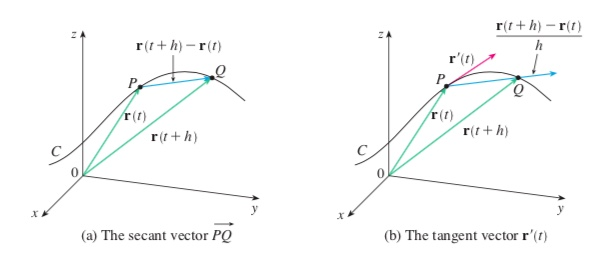
\includegraphics[scale=0.4]{figures_mvc/tangent_vector_secant_vector}
\end{center}
\caption{The derivative $\bbr'(t)$ is the tangent vector to the curve $\bbr$ at $\bbr(t)$.}
\end{figure}
The next theorem shows that we can compute the derivative of a vector-valued function in terms of the derivatives of its component functions.

\begin{thm}[Derivative of a vector-valued function]\label{thm:derivative_of_a_vector-valued_function}
	The derivative of a vector-valued function $\bbr(t)=(r_1(t),r_2(t),r_3(t))$ is given by 
	\begin{align*}
		\bbr'(t)=(r_1'(t),r_2'(t),r_3'(t)).
	\end{align*}
\end{thm}

\begin{pf}
By Theorem \ref{thm:limit_of_a_vector-valued_function}
\begin{align*}
	\bbr'(t)&=\lim_{h \to 0}\frac{\bbr(t+h)-\bbr(t)}{h} \\
	&=\lim_{h \to 0}\frac{(r_1(t+h),r_2(t+h),r_3(t+h))-(r_1(t),r_2(t),r_3(t))}{h} \\
	&=\lim_{h \to 0}\frac{(r_1(t+h)-r_1(t),r_2(t+h)-r_2(t),r_3(t+h)-r_3(t))}{h} \\
	&=\lim_{h \to 0}\left(\frac{r_1(t+h)-r_1(t)}{h},\frac{r_2(t+h)-r_2(t)}{h},\frac{r_3(t+h)-r_3(t)}{h}\right) \\
	&=\left(\lim_{h \to 0}\frac{r_1(t+h)-r_1(t)}{h},\lim_{h \to 0}\frac{r_2(t+h)-r_2(t)}{h},\lim_{h \to 0}\frac{r_3(t+h)-r_3(t)}{h}\right) \\
	&=(r_1'(t),r_2'(t),r_3'(t)).
\end{align*}	
\end{pf}

\begin{example}
Let $\bbr(t)=(\sin t,\cos t,e^t)$. Then
\begin{align*}
	\bbr'(\varphi(t))&=((\sin t)',(\cos t)',(e^t)') \\
	&=(\cos t, - \sin t, e^t).
\end{align*}	
\end{example}

\begin{thm}[Differentiation formulas]
	Let $\bu,\bv$ be differentiable vector-valued functions into $\R^n$, $c$ a constant, and $\varphi:\mathbb{R} \to \mathbb{R}$ a real-valued function. Then
\begin{enumerate}[(1)]
		\item $[\bu(t)+\bv(t)]'=\bu'(t)+\bv'(t)$
		\item $[c\bu(t)]'=c\bu'(t)$
		\item $[\varphi(t)\bu(t)]'=\varphi'(t)\bu(t)+\varphi(t)\bu'(t)$
		\item $[\bu(t)\cdot \bv(t)]'=\bu'(t)\cdot \bv(t)+\bu(t) \cdot \bv'(t)$
		\item $[\bu(t)\times \bv(t)]'=\bu'(t)\times \bv(t)+\bu(t) \times \bv'(t)$ (for $n=3$)
		\item $[\bu(\varphi(t))]'=\varphi'(t)\bu'(\varphi(t))$
	\end{enumerate}	
\end{thm}

\begin{pf}
The proof follows immediately from Theorem \ref{thm:derivative_of_a_vector-valued_function} and the corresponding properties for real-valued functions.
\end{pf}


\begin{defn}[Higher derivatives]
	\begin{enumerate}[(a)]
		\item The \emph{second derivative}, $\bbr''$, of a vector-valued function $\bbr$ is the derivative of $\bbr'$: $\bbr''=(\bbr')'$. Thus,
\begin{align*}
	\bbr''(t)=(f''(t), g''(t), h''(t))
\end{align*}
Similarly, for $k$ a positive integer, the $k$th derivative of $\bbr$ is given by the formula
\begin{align*}
	\bbr^{(k)}(t)=(f^{(k)}(t), g^{(k)}(t), h^{(k)}(t)).
\end{align*}
\item A vector-valued function is said to be \emph{of class $\mathscr{C}^k$} if its first $k$ derivatives exist and are continuous and \emph{of class $\mathscr{C}^\infty$} if all of its derivatives exist. Functions in the class $\mathscr{C}^\infty$ are also called \emph{smooth}.
	\end{enumerate}
\end{defn}

\subsubsection{Integrals of Vector valued functions}
Similar to derivatives, we define the integral of a vector-valued function in terms of the integrals of its component functions.

\begin{defn}[Integral of a vector-valued function]
	If $\bbr(t)=(r_1(t),\dots,r_n(t))$ is a vector-valued function, then
	\begin{align*}
		\int_a^b \bbr(t)dt=(\int_a^b r_1(t)dt,\cdots,\int_a^b r_n(t)dt).
	\end{align*}
	Indefinite integrals are defined similarly.
\end{defn}

\begin{example}
\begin{enumerate}[(a)]
	\item Let $\bbr(t)=(\cos t, 1, -2t)$. Then
\begin{align*}
	\int (\cos t, 1, -2t)dt&=\left(\int \cos t dt,\int dt,-\int 2t dt\right) \\
	&=(\sin t+c_1,t+c_2,-(t^2+c_3)) \\
	&=(\sin t, t, -t^2)+(c_1,c_2,-c_3).
\end{align*}
\item Now a definite integral:
\begin{align*}
	\int_0^\pi (\cos t, 1, -2t)dt&=\left(\int_0^\pi \cos t dt,\int_0^\pi dt,-\int_0^\pi 2t dt\right) \\
	&=(\sin t|_0^\pi,t|_0^\pi,-t^2|_0^\pi) \\
	&=(0-0,\pi-0,-(\pi^2-0^2)) \\
	&=(0,\pi,-\pi^2).
\end{align*}
\end{enumerate}	
\end{example}

\begin{exercise}
	Solve the first order differential equation
	\begin{align*}
		\bbr'(t)=(\cos t,-\sin t,1)
	\end{align*}
	subject to the initial condition $\bbr(0)=(2,0,1)$.
\end{exercise}

{\color{red}
\begin{solution}
	This differential equation can be solved by integrating with respect to $t$:
	\begin{align*}
		\bbr(t)&=\int \bbr'(t)dt \\
		&=(\int \cos t dt,-\int \sin t dt, \int dt) \\
		&=(\sin t, \cos t, t)+(c_1,c_2,c_3).
	\end{align*}
	The initial condition says that
	\begin{align*}
		\bbr(0)&=(\sin 0, \cos 0, 0)+(c_1,c_2,c_3) \\
		&=(0,1,0)+(c_1,c_2,c_3) \\
		&=(c_1,c_2+1,c_3) \\
		&=(2,0,1),
	\end{align*}
	and therefore
	\begin{align*}
		c_1&=2 \\
		c_2+1&=0 \\
		c_3&=1.
	\end{align*}
	Thus, the solution to the differential equation is
	\begin{align*}
		\bbr(t)&=(\sin t, \cos t, t)+(2,-1,1) \\
		&=(\sin t+2, \cos t-1,t+1).
	\end{align*}
	
\end{solution}}

\newpage 

\subsection{Parametrized Curves}
We will now focus on a special class of vector-valued functions, which model the motion of a particle through space. Our interest will primarily be in the geometry of the particle's trajectory.

\begin{defn}[Parametrized curve]
	Let $I$ be an interval. A \emph{parametrized curve} is a smooth mapping $\bbr:I \to \mathbb{R}^n$. For $n=2$, a curve is also called a \emph{plane curve} while for $n=3$ it is also called a \emph{space curve}. The variable $t$ is called the \emph{parameter}. The image $\bbr(I) \subseteq \R^n$ is called the \emph{trace} of the curve $\bbr$. \footnote{The \emph{image of $I$ under $\bbr$} is the set $\bbr(I)=\{\bbr(t):t \in I\}$.}
\end{defn}

\begin{remark}
Every interval in $\R$ is of one of the following forms:
\begin{align*}
	(-\infty,b), (-\infty,b], (a,b), [a,b), (a,b], [a,b],[a,\infty), (a,\infty).
\end{align*}
If $I$ is an interval containing boundary points, such as $[a,b]$, then we define $f'(a)$ as the right-hand limit
\begin{align*}
	f'(a)=\lim_{h \to 0^+}\frac{f(a+h)-f(a)}{h}
\end{align*}
and, $f'(b)$ as the left-hand limit
\begin{align*}
	f'(b)=\lim_{h \to 0^-}\frac{f(b+h)-f(b)}{h}.
\end{align*}
\end{remark}

To avoid the proliferation of primes in what follows, we will use the following physical terminology.
\begin{defn}[Velocity, speed, accleration]
	\begin{enumerate}[(a)]
		\item We will call the tangent vector $\bbr'(t)$ the \emph{velocity} at $t$. We call its length $||\bbr'(t)||$ the \emph{speed} at $t$.
		\item We call the vector $\bbr''(t)$ the \emph{acceleration} at $t$.
	\end{enumerate}
	From now on we will write $\bv(t) \equiv \bbr'(t), ||\bv(t)||\equiv ||\bbr'(t)||$, and $\ba(t)\equiv \bbr''(t)$.
\end{defn}


\newpage

\begin{example}
The graph of any smooth function $y=f(x)$ can be written as a parametrized curve by defining
\begin{align*}
	\bbr:\R &\to \R^2 \\
	\bbr(t)&=(t,f(t)).
\end{align*}
For example, the function $y=x^2$ can be written the parametrized curve $\bbr(t)=(t,t^2)$ for all $-\infty < t < \infty$.	The trace of a plane curve can be plotted in \emph{Mathematica} as shown below:

\begin{figure}[h]
	\begin{center}
		\includegraphics[scale=0.5]{figures_mvc/parab_param_plot}
	\end{center}
	\caption{The trace of the plane curve $\bbr(t)=(t,t^2)$.}
\end{figure} 

The particle moves down the parabola from the upper left starting at $t=-\infty$, reaches the origin at $t=0$, and then continues up the parabola to the upper right for all $t>0$. \footnote{Some nice animations of parametrized curves can be found at \href{https://demonstrations.wolfram.com/ParametricTrace/}{https://demonstrations.wolfram.com/ParametricTrace/}.}
\end{example}


\begin{exercise}
Sketch the trace of the plane curve $\bbr(t)=(t^2-2t,t+1)$, $-\infty < t < \infty$ in by making a table of the coordinates $(x(t),y(t))$ for integer values of $t$ from $-2 \leq t \leq 4$. Compare your sketch with the curve produced in \emph{Mathematica} using the ``ParametricPlot" command.	
\end{exercise}
{\color{red}
\begin{solution}
	The curve is a parabola, which we can confirm by eliminating $t$ as follows. First, solve for $t$ in terms of $y$ to obtain
\begin{align*}
	y=t+1 \implies y-1=t.
\end{align*}
Substituting into $x(t)$ then gives $x$ in terms of $y$:
\begin{align*}
	x=t^2-2t=(y-1)^2-2(y-1)=y^2-4y+3=(y-2)^2-1.
\end{align*}
which is the equation of a parabola in vertex form, with vertex at $(x,y)=(-1,2)$. 

\begin{figure}[h]
	\begin{center}
		\includegraphics[scale=0.5]{figures_mvc/sideways_parab_mma}
	\end{center}
	\caption{The trace of the plane curve $\bbr(t)=(t^2-2t,t+1)$ from $-2 \leq t \leq 4$.}
\end{figure}

The particle travels upwards along the parabola from $t=-\infty$, reaches the vertex at $t=1$, and then continues upward to the right for $t>0$.
\end{solution}}

\newpage

\begin{example}\label{ex:unit_circ}
Consider the following three plane curves 
\begin{enumerate}[(1)]
	\item $\bbr_1(t)=(\cos t, \sin t), 0 \leq t \leq 2\pi$, 
	\item $\bbr_2(t)=(-\sin 2t, \cos 2t), 0 \leq t \leq 2\pi$,
	\item $\bbr_3(t)=(\cos(-t), \sin(-t)), 0 \leq t \leq 2\pi$.
\end{enumerate}	
For all three curves, $x(t)^2+y(t)^2=1$, so the trace of each curve is the unit circle. However, as trajectories of a particle, they are different. The reader can easily verify the following by making a table for each curve and sketching the trace:
\begin{enumerate}[(1)]
	\item In $\bbr_1$, the particle begins at $(x,y)=(1,0)$ at $t=0$ and completes one full circle, moving in the counterclockwise direction.
	\item In $\bbr_2$, the particle begins at $(x,y)=(0,1)$ at $t=0$ and completes \emph{two} full circles, moving in the counterclockwise direction.
	\item In $\bbr_3$, the particle begins at $(x,y)=(1,0)$ at $t=0$ and completes one full circle, moving in the \emph{clockwise} direction.
\end{enumerate}
\begin{figure}[h]
	\begin{center}
		\includegraphics[scale=0.4]{figures_mvc/circ_param_plot_mma}
	\end{center}
	\caption{The trace of the curves $\bbr_1,\bbr_2,\bbr_3$.}
\end{figure}
\end{example}

\newpage 

The previous example shows that a parametrized curve is more than just the trace: it is the trace together with a choice of how to traverse the trace of curve.

\begin{example}
Consider now the trace of the plane curve $\bbr(t)=(t^3,t^2)$, $-\infty<t<\infty$.

\begin{figure}[h]
	\begin{center}
		\includegraphics[scale=0.4]{figures_mvc/cusp_mma}
	\end{center}
\end{figure}
Since the component functions are smooth, the reader may be surprised by the cusp at the origin. Solving for $y$ in terms of $x$ by eliminating $t$, we find that $y=x^{2/3}$, which is indeed not differentiable at the origin. Note that $\bv(t)=(3t^2,2t)\neq (0,0)$ everywhere except the origin, where the tangent vector vanishes.
\end{example}
 
\begin{defn}[Regular curve]
	Let $\bbr:I \to \R^n$ be a parametrized curve.
	\begin{enumerate}[(a)]
		\item A point where $\bv(t)={\bf 0}$ is called a \emph{singular point}, while a point where $\bv(t) \neq {\bf 0}$ is called a \emph{regular point}.
		\item A \emph{regular curve} is a curve with no singular points; that is, it is a curve for whice $\bv(t) \neq {\bf 0}$ for all $t \in I$.
	\end{enumerate}
\end{defn}
In our study of the differential geometry of curves, we will assume our curve has a tangent vector at every point. Thus, from now on we will assume all curves are regular.

\subsection{Reparametrizations}
Recall the three regular curves from Example \ref{ex:unit_circ}:
\begin{enumerate}[(1)]
	\item $\bbr_1(t)=(\cos t, \sin t), 0 \leq t \leq 2\pi$, 
	\item $\bbr_2(t)=(-\sin 2t, \cos 2t), 0 \leq t \leq 2\pi$,
	\item $\bbr_3(t)=(\cos(-t), \sin(-t)), 0 \leq t \leq 2\pi$.
\end{enumerate}	
We have noticed that all three curves have exactly the same trace; namely, the unit circle. If we are only interested in the geometry of the trace of the curve, then we should view all parametrized curves with the same trace as equivalent. We now formalize this idea.

First, notice that if we define the function
\begin{align*}
	\varphi:[0,2\pi] \to [0,2\pi]
\end{align*}
by 
\begin{align*}
	\varphi(t)=2t+\frac{\pi}{2}
\end{align*}
then we see that $\bbr_2$ is equal to the composition $\bbr_2=\bbr_1 \circ \varphi$, since for all $t \in [0,2\pi]$
\begin{align*}
	\bbr_1(\varphi(t))&=(\cos(2t+\frac{\pi}{2}),\sin(2t+\frac{\pi}{2})) \\
	&=(\cos(2t)\underbrace{\cos(\frac{\pi}{2})}_{=0}-\sin(2t)\underbrace{\sin(\frac{\pi}{2})}_{=1}, \sin(2t)\underbrace{\cos(\frac{\pi}{2})}_{=0}+\cos(2t)\underbrace{\sin(\frac{\pi}{2})}_{=1}) \\
	&=(-\sin(2t),\cos(2t)) \\
	&=\bbr_2(t).
\end{align*}

To understand this relationship, recall that a parametrized curve $\bbr(t)$ is a function which gives the position of the particle at time $t$, with respect to a given clock. If $\varphi$ denotes the time with respect to a different clock, then $\bbr(\varphi)$ gives the position of the particle at time $\varphi$. The particles follow the same trajectory, but are at different positions at different times if the two clocks are not synchronized. In this example, the clocks are related by $\varphi=2t+\frac{\pi}{2}$; that is, the $\varphi$-clock is $\frac{\pi}{2}$ seconds ahead of the $t$-clock (since $\varphi=\frac{\pi}{2}$ when $t=0$), and runs half as fast (since if the time interval between two successive ticks of the $t$-clock is $\Delta t=1$ s, then the time interval between two successive ticks of the $\varphi$-clock is  $\Delta \varphi=2\Delta t=2$ s; that is, if the $t$-clock ticks once every second, then the $\varphi$-clock ticks once every two seconds). Thus if $\bbr_1(t)$ describes a single trip around the unit circle in the counterclockwise sense at unit speed, then, with respect to the $t$-clock, $\bbr_1(\varphi)=\bbr_2(t)$ describes a particle that is already at $(0,1)$ when $t=0$ and completes two trips around the circle at double speed in $2\pi$ seconds.

\begin{exercise}\label{ex:orient_reve}
Verify that by defining $\varphi:[0,2\pi] \to [0,2\pi]$ by $\varphi(t)=2\pi-t$, then $\bbr_3=\bbr_1 \circ \varphi$. Interpret this as above.	
\end{exercise}

{\color{red}
\begin{solution}
We see that $\bbr_1(\varphi(t))=(\cos(2\pi-t),\sin(2\pi-t))=(\cos(-t),\sin(-t))=\bbr_3(t)$ for all $t$. The $\varphi$-clock is related to the $t$-clock by ``time-reversal"; that is, the clocks run at the same speed, but the $\varphi$ clock runs backwards with respect to the $t$-clock, since $\varphi(t)$ is a decreasing function of $t$ with $\varphi(0)=2\pi$ and $\varphi(2\pi)=0$.	
\end{solution}
}
\begin{defn}[Reparametrization]
	Let $\bbr:I \to \mathbb{R}^n$ be a regular curve. A \emph{reparametrization} of $\bbr$ is a function of the form $\widetilde{\bbr}=\bbr \circ \varphi:\tilde{I} \to \mathbb{R}^n$, where $\tilde{I}$ is an interval and $\varphi:\tilde{I} \to I$ is a smooth bijection with nowhere vanishing derivative ($\varphi'(t) \neq 0$ for all $t \in \tilde{I}$). \footnote{While in each of the examples above we had $\varphi:\tilde{I} \to I$ with $\tilde{I}=I$, these intervals need not be the same. For instance, in Example \ref{ex:orient_reve}, we could have instead taken $\varphi:[0,2\pi] \to [-2\pi,0]$ where $\varphi(t)=-t$.}
\end{defn}

\begin{figure}[h]
	\begin{center}
		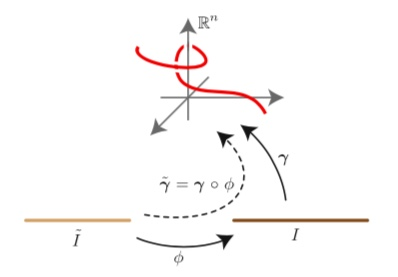
\includegraphics[scale=0.5]{figures_mvc/reparametrization}
	\end{center}
	\caption{A reparametrization $\widetilde{\bbr}=\bbr \circ \varphi$ of a curve $\bbr$.}
\end{figure}

\begin{remark}
Note that the hypotheses on $\varphi$ are all required to ensure that $\widetilde{\bbr}=\bbr \circ \varphi$ has the same trace as $\bbr$:
\begin{itemize}
	\item The requirement that $\varphi$ is smooth ensures that $\widetilde{\bbr}$ is smooth, since the composition of smooth functions is smooth.
	\item The requirement that $\varphi$ is a bijection is also essential. If $\varphi$ is not surjective, then the trace of $\widetilde{\bbr}$ will only be a proper subset of the trace of $\bbr$. If $\varphi$ is not injective, then $\widetilde{\bbr}$ will have self-intersections at points where $\bbr$ does not (since if $\varphi(t_1)=\varphi(t_2)$ for $t_1 \neq t_2$, then even if $\bbr(t_1) \neq \bbr(t_2)$, we will have $\widetilde{\bbr}(\varphi(t_1))=\widetilde{\bbr}(\varphi(t_2))$). Thus, if $\varphi$ is not a bijection, then the two curves won't have the same trace.
	\item The requirement that $\varphi'(t) \neq 0$ for all $t$ ensures that $\widetilde{\bbr}(t)$ is regular, since if $\bbr(t)$ is regular and $\varphi'(t) \neq 0$, then by the chain rule
	\begin{align*}
		\widetilde{\bv}(t)=\varphi'(t)\bbr'(t) \neq 0.
	\end{align*}
\end{itemize}
\end{remark}

\begin{prop}[Reparametrized curves are equivalent]
The relation $\widetilde{\bbr} \sim \bbr$ if $\widetilde{\bbr}$ is a reparametrization of $\bbr$ is an equivalence relation. 	
\end{prop}

\begin{pf}
	\begin{enumerate}[(1)]
		\item (Reflexivity) Let $\bbr:I \to \R^n$ be a parametrized curve. Take $\varphi=id_I:T \to I$ to be the identity map on $I$. This is a smooth bijection, and since $id_I(t)=t$, $id_I'(t)=1 \neq 0$ for all $t \in I$. Since $\bbr=\bbr \circ id_I$, $\bbr \sim \bbr$. Thus, $\sim$ is reflexive.
		\item (Symmetry) Suppose $\bbr:I \to \R^n$ and $\widetilde{\bbr}:\tilde{I} \to \R^n$ are parametrized curves with $\widetilde{\bbr} \sim \bbr$. Then there exists a smooth bijection $\varphi: \tilde{I} \to I$ with $\varphi'(t) \neq 0$ for all $t \in \tilde{I}$ such that $\widetilde{\bbr}=\bbr \circ \varphi$. It follows from the Inverse Function Theorem that $\varphi$ has a smooth inverse, $\varphi^{-1} :I \to \tilde{I}$, where $(\varphi^{-1})'(t)=1/\varphi'(t)$ Since $\varphi'(t)$ is never zero, neither is $(\varphi^{-1})'(t)$. \footnote{The \emph{Inverse Function Theorem} states that if $\varphi:I \to \R$ is continuously differentiable with $\varphi'(t_0) \neq 0$ then $\varphi$ is invertible in a neighborhood of $t_0$, the inverse is continuously differentiable, and the derivative of the inverse function at $b=\varphi(t_0)$ is the reciprocal of the derivative of $\varphi$ at $t_0$. Applying this to the $k$-th derivative, it follows as a corollary that we can replace ``continuously differentiable" everywhere in the theorem above by ``smooth". For a regular curve $\varphi'(t)$ is never zero on $I$, so $\varphi$ must be either increasing or decreasing on $I$. Either way $\varphi$ is 1-1 on all of $I$, and therefore the ``neighborhood" of $t_0$ appearing in the theorem is all of $I$.} Then 
		\begin{align*}
			\widetilde{\bbr} \circ \varphi^{-1}&=\bbr \circ \varphi^{-1} \circ \varphi \\
			&=\bbr \circ id_I \\
			&=\bbr. 
		\end{align*}
		 This proves that $\widetilde{\bbr} \sim \bbr$ implies that $\bbr \sim \widetilde{\bbr}$. Thus, $\sim$ is symmetric.
		\item (Transitivity) Let
		\begin{align*}
			\bbr_1:I_1 &\to \R^n, \\
			\bbr_2:I_2 &\to \R^n, \\
			\bbr_3:I_3 &\to \R^n, \\
		\end{align*}
		be parametrized curves and suppose $\bbr_1 \sim \bbr_2$ and $\bbr_2 \sim \bbr_3$. Then there exist smooth bijections 
		\begin{align*}
			\varphi:I_2 &\to I_1, \\
			\psi:I_3 &\to I_2
		\end{align*} 
		with nowhere vanishing first derivatives such that
		\begin{align*}
			\bbr_2&=\bbr_1 \circ \varphi, \\
			\bbr_3&=\bbr_2 \circ \psi
		\end{align*}
		Then $\varphi \circ \psi:I_3 \to I_1$ is a smooth bijection with nowhere vanishing derivative such that
		\begin{align*}
			\bbr_3=\bbr_1 \circ \varphi \circ \psi.
		\end{align*}
		Thus, $\bbr_1 \sim \bbr_3$.
	\end{enumerate}
	This shows that $\sim$ is reflexive, symmetric, and transitive, and is therefore an equivalence relation.
\end{pf}
\begin{defn}[Curve]
	The we call the equivalence class
	\begin{align*}
		[\bbr]\equiv \{\widetilde{\bbr}:\widetilde{\bbr}=\bbr \circ \varphi \text{ for some } \varphi\}
	\end{align*} 
 a \emph{curve} in $\R^n$. Any parametrized curve $\widetilde{\bbr}(t)$ in $[\bbr]$ is said to be a \emph{representative} of the equivalence class $[\bbr]$. 
\end{defn}

Let $\bbr(t)$ be a parametrized curve and let $\widetilde{\bbr}=\bbr \circ \varphi$ be a reparametrization of $\bbr(t)$. Since $\varphi'(t)$ is nowhere 0, $\varphi$ must be either monotonically increasing ($\varphi'>0$) or monotonically decreasing ($\varphi'<0$) on all of $\tilde{I}$.

\begin{defn}[Oriented curves]
A reparametrization $\widetilde{\bbr}=\bbr \circ \varphi$ is said to be \emph{orientation-preserving} if $\varphi'>0$ and \emph{orientation-reversing} if $\varphi'<0$. Thus, each curve $[\bbr]$ is partitioned into two subsets
\begin{align*}
	[\bbr]_+&=\{\widetilde{\bbr}:\widetilde{\bbr}=\bbr \circ \varphi \text{ with } \varphi'>0\}, \\
	[\bbr]_-&=\{\widetilde{\bbr}:\widetilde{\bbr}=\bbr \circ \varphi \text{ with } \varphi'<0\}. \\
\end{align*}
Each subset is called an \emph{oriented curve}. A choice of orientation of a curve $[\bbr]$ is a choice of one of these two subsets.
\end{defn}

\begin{exercise}
Consider again three parametrized curves from Example \ref{ex:unit_circ} and :
\begin{enumerate}[(1)]
	\item $\bbr_1(t)=(\cos t, \sin t), 0 \leq t \leq 2\pi$, 
	\item $\bbr_2(t)=(-\sin 2t, \cos 2t), 0 \leq t \leq 2\pi$,
	\item $\bbr_3(t)=(\cos(-t), \sin(-t)), 0 \leq t \leq 2\pi$.
\end{enumerate}	
Which of these curves have the same orientation?
\end{exercise}

{\color{red}
\begin{solution}
	We have seen that $\bbr_2=\bbr_1 \circ \varphi$ where $\varphi(t)=2t+\frac{\pi}{2}$. Since $\varphi'(t)=2>0$, these two curves have the same orientation (i.e., they are representatives of the same oriented curve). We also saw that $\bbr_3=\bbr_1 \circ \psi$ where $\psi(t)=2\pi-t$. Since $\psi'(t)=-1<0$, these two curves have opposite orientation.
\end{solution}
}

\subsection{Arc Length}
We have just seen that a given curve can be parametrized in many ways. Out of these many options, there is a natural choice for the parameter $t$, namely, the \emph{arc length} measured from any point $\bbr_0$ on the curve. This is because the arc length is an \emph{invariant} of the curve, which is independent of the parametrization. For a curve given by the graph of a function $y=f(x)$, the arc length from $a$ to $b$ is given by
\begin{align}\label{eq:arc_leng_f_x}
	s=\int_a^b\sqrt{1+(f'(x))^2}dx.
\end{align}
Writing the function as a parametrized curve $\bbr(t)=(t,f(t))$, we have $\bv(t)=(1,f'(t))$ and $||\bv(t)||=\sqrt{1+(f'(t))^2}$, so we can write Equation \eqref{eq:arc_leng_f_x} as
\begin{align}\label{eq:arc_length_gen}
	s=\int_a^b||\bv(t)||dt.
\end{align}

How do we compute the arc length if $\bbr(t)$ is not the graph of a function?  If $\bbr(t)$ is not the graph of a function, it turns out that Equation \eqref{eq:arc_length_gen} is still valid.  In this case, we obtain the formula as the limit of a sequence of polygonal approximations of the curve. For those interested in the details, see Appendix \ref{app:arc_length}. 

\begin{defn}{Arc length}\label{def:arc_length}
Let $\bbr:[a,b] \to \R^n$ be a regular curve. We define the \emph{arc length} between the points $\bbr(a)$ and $\bbr(b)$ on the curve by
\begin{align*}
	s=\int_a^b||\bv(t)||dt.
\end{align*}	
\end{defn}

\begin{example}\label{ex:unit_circl_ex}
We now compute the arc length along the portion of the unit circle from $(1,0)$ to $(0,1)$. If we use the parametrization
\begin{align*}
	\bbr_1(t)=(\cos t,\sin t), \hspace{0.25cm} 0 \leq t \leq \frac{\pi}{2},
\end{align*}	
then we have
\begin{align*}
	\bv_1(t)&=(-\sin t,\cos t), \\
	||\bv_1(t)||&=\sqrt{(-\sin t)^2+(\cos t)^2}=\sqrt{1}=1.
\end{align*}
Equation \eqref{eq:arc_length_gen} then gives
\begin{align*}
	s=\int_0^{\frac{\pi}{2}}||\bv_1(t)||dt=\int_0^{\frac{\pi}{2}}dt=\frac{\pi}{2}.
\end{align*}
\end{example}

\begin{exercise}
Use the parametrization $\bbr_2(t)=(\cos(2t),\sin(2t))$, $0 \leq t \leq \frac{\pi}{4}$ to compute the arc length of the same portion of the unit circle as in Example \ref{ex:unit_circl_ex}. Verify that you get the same answer.	
\end{exercise}

{\color{red}
\begin{solution}
	Using the parametrization $\bbr_2(t)=(\cos(2t),\sin(2t))$, $0 \leq t \leq \frac{\pi}{4}$, we have
	\begin{align*}
		\bv_2(t)&=(-2\sin(2t),2\cos(2t)), \\
		||\bv_2(t)||&=\sqrt{4\sin^2(2t)+4\cos^2(2t)}=\sqrt{4(\sin^2(2t)+\cos^2(2t))}=\sqrt{4}=2
	\end{align*} 
	and therefore
	\begin{align*}
		s=\int_0^{\frac{\pi}{4}}||\bv_2(t)||dt=2\int_0^{\frac{\pi}{4}}dt=2\cdot \frac{\pi}{4}=\frac{\pi}{2}.
	\end{align*}
\end{solution}}

\begin{exercise}
A \emph{logarithmic spiral} is a plane curve of the form $\bbr(t)=c(e^{\lambda t}\cos t,e^{\lambda t}\sin t)$, $t \in \mathbb{R}$ where $c,\lambda \in \mathbb{R}$ and $c \neq 0$. Below is the restriction of $\bbr(t)$ to $[0,\infty)$ with $\lambda <0$.	

\begin{figure}[h]
	\begin{center}
		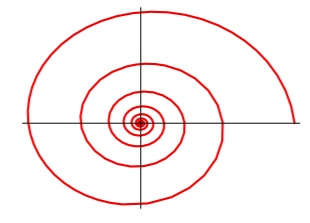
\includegraphics[scale=0.5]{figures_mvc/log_spiral}
	\end{center}
\end{figure}
Use an improper integral to prove that such a restriction has finite arc length even though it makes infinitely many loops around the origin.
\end{exercise}

{\color{red}
\begin{solution}
	We have
	\begin{align*}
		\bv(t)&=c(\lambda e^{\lambda t}\cos t-e^{\lambda t}\sin t,\lambda e^{\lambda t}\sin t+e^{\lambda t}\cos t) \\
		&=ce^{\lambda t}(\lambda \cos t-\sin t, \lambda \sin t+\cos t)
	\end{align*}
	and therefore
	\begin{align*}
		||\bv(t)||&=|c|e^{\lambda t}\sqrt{(\lambda \cos t-\sin t)^2+(\lambda \sin t+\cos t)^2} \\
		&=|c|e^{\lambda t}\sqrt{\lambda^2\cos^2 t+\sin^2 t-2\lambda \sin t \cos t+\lambda^2\sin^2 t+ \cos ^2 t+2\lambda \sin t\cos t} \\
		&=|c|e^{\lambda t}\sqrt{\lambda^2+1}.
	\end{align*}
	The arc length is then given by the integral
	\begin{align*}
		s=\int_0^\infty ||\bv(t)||dt=|c|\sqrt{\lambda^2+1}\int_0^\infty e^{-|\lambda|t}dt.
	\end{align*}
	Substituting
	\begin{align*}
		u=-|\lambda|t, \ du=-|\lambda|dt,
	\end{align*}
	this becomes
	\begin{align*}
		s&=-\frac{|c|\sqrt{\lambda^2+1}}{|\lambda|}\int_0^{-\infty}e^{u}du \\
		&=-\frac{|c|\sqrt{\lambda^2+1}}{|\lambda|}\lim_{k \to -\infty}(e^k-1) \\
		&=-\frac{|c|\sqrt{\lambda^2+1}}{|\lambda|}(0-1) \\
		&=\frac{|c|\sqrt{\lambda^2+1}}{|\lambda|}.
	\end{align*}
\end{solution}}

\begin{prop}[Invariance of arc length]
	The arc length is independent of parametrization.
\end{prop}

\begin{pf}
Let $\widetilde{\bbr}=\bbr \circ \varphi$ be a reparametrization of $\bbr$. Then since
\begin{align*}
\widetilde{\bv}(t)&=[\bbr(\varphi(t))]'=\varphi'(t)\bv(\varphi(t)),
\end{align*}
we have
\begin{align*}
	s&=\int_{t_0}^{t_1}||\widetilde{\bv}(t)||dt \\
	&=\int_{t_0}^{t_1}||\varphi'(t)\bv(\varphi(t))||dt \\
	&=\int_{t_0}^{t_1}||\bv(\varphi(t))|| \ |\varphi'(t)|dt \\
\end{align*}	
If $\varphi'(t)>0$, then $|\varphi'(t)|=\varphi'(t)$ and by substituting
\begin{align*}
	u=\varphi(t), \ du=\varphi'(t)dt
\end{align*}
we obtain
\begin{align*}
	s=\int_{\varphi(t_0)}^{\varphi(t_1)}||\bv(u)||du.
\end{align*}
If $\varphi'(t)<0$, then $|\varphi'(t)|=-\varphi'(t)$ and the same substitution gives
\begin{align*}
	s=-\int_{\varphi(t_0)}^{\varphi(t_1)}||\bv(u)||du=\int_{\varphi(t_0)}^{\varphi(t_1)}||\bv(u)||du.
\end{align*}
\end{pf}

\begin{prop}[Any regular curve can be parametrized by arc length]
	Any regular curve $\bbr:I \to \R^n$ can be parametrized by arc length.
\end{prop}

\begin{pf}
Choose $t_0 \in I$ and consider the arc length function $s:I \to \R$ defined by
\begin{align*}
	s(t)=\int_{t_0}^t||\bv(u)||du. 
\end{align*}	
Let $\tilde{I}=s(I)$ denote the image of $I$ under $s$. By the Fundamental Theorem of Calculus, $s'(t)=||\bv(t)|| \neq 0$ (since the curve is regular), so by the Inverse Function Theorem $s$ has an inverse $\varphi:\tilde{I} \to I$, which is also a smooth bijection with a nowhere-vanishing derivative. Then $\widetilde{\bbr}=\bbr \circ \varphi$ is parametrized by arc length, since $\bbr(\varphi(s))$ is the position of a point along the curve at the time when it achieves arc length $s$ measured from $t_0$.
\end{pf}

\begin{example}\label{ex:helix_param_by_arc_length}
Consider the helix $\bbr(t)=(\cos t, \sin t, t)$, $t \in \R$. 
\begin{figure}[h]
	\begin{center}
		\includegraphics[scale=0.5]{figures_mvc/helix_fig}
	\end{center}
\end{figure}

 Let us reparametrize the helix with respect to the arc length measured from $(1,0,0)$ in the direction of increasing $t$. Since $\bbr(0)=(1,0,0)$, following the proof above we define
\begin{align*}
	s(t)=\int_0^t||\bv(u)||du.
\end{align*}
Since $\bv(u)=(-\sin u,\cos u,1)$, we have $||\bv(u)||=\sqrt{2}$ and therefore
\begin{align*}
	s(t)&=\int_0^t||\bv(u)||du \\
	&=\sqrt{2}\int_0^t du \\
	&=\sqrt{2}t.
\end{align*}
The inverse function is then easily obtained:
\begin{align*}
	\varphi(s)=\frac{s}{\sqrt{2}}
\end{align*}
and 
\begin{align*}
	\bbr(\varphi(s))=\left(\cos\left(\frac{s}{\sqrt{2}}\right),\sin\left(\frac{s}{\sqrt{2}}\right),\frac{s}{\sqrt{2}}\right).
\end{align*}
\end{example}

\begin{example}
Let's reparametrzie the plane curve $\bbr(t)=(\cos(3t),\sin(2t))$ with respect to arc length measured from $(1,0)$ in the direction of increasing $t$. Since
	\begin{align*}
		\bv(t)&=(-3\sin(3t),2\cos(2t)) \\
		||\bv(t)||&=\sqrt{9\sin^2(3t)+4^2\cos(2t)},
	\end{align*}
	the arc length function is given by
	\begin{align*}
		s(t)=\int_0^t\sqrt{9\sin^2(3t)+4\cos^2(2t)}dt
	\end{align*}
	This integral cannot be evaluated in closed form. This example illustrates that, while our proof gave an explicit method to parametrize any curve by arc length, in practice it is usually not computationally reasonable to implement. However, the fact that every curve can be parametrized by arc length is very important for theoretical purposes, as we will see in the following sections.
\end{example}

\begin{prop}
	A curve parametrized by arc length is a \emph{unit speed curve}; that is, $||\bv(t)||=1$ for all $t \in I$.
\end{prop}

\begin{proof}
	If $\bbr$ is parametrized by arc length, then by the Fundamental Theorem of Calculus
	\begin{align*}
		s'(t)=\frac{d}{dt}\int_{t_0}^t||\bv(u)||du=||\bv(t)||=1.
	\end{align*}
	Conversely, suppose $||\bv(t)||=1$ for all $t$. Then
	\begin{align*}
		s(t)=\int_{t_0}^t||\bv(u)||du=\int_{t_0}^tdu=t-t_0
	\end{align*}
	so $t$ is equal to the arc length accumulated from the point $t_0$.
\end{proof}

\begin{exercise}
Verify that the helix parametrized by arc length in Example \ref{ex:helix_param_by_arc_length} is a unit speed curve.	
\end{exercise}

{\color{red}
\begin{solution}
We have $\bv(s)=\frac{1}{\sqrt{2}}(-\sin(\frac{s}{\sqrt{2}}), \cos(\frac{s}{\sqrt{2}}),1)$ and therefore 
\begin{align*}
	||\bv(s)||&=\frac{1}{\sqrt{2}}\sqrt{\sin^2(\frac{s}{\sqrt{2}})+\cos^2(\frac{s}{\sqrt{2}})+1} \\
	&=\frac{1}{\sqrt{2}}\sqrt{2} \\
	&=1.
\end{align*}	
\end{solution}
}

\begin{exercise}
Parametrize each of the following curves by arc length (measured from $t=0$) and verify that $||\bv(s)||=1$ for all $s$.
\begin{enumerate}[(1)]
	\item Helix: $\bbr(t)=(a\cos t, a \sin t, bt), \ -\infty<t<\infty, \ a,b \text{ fixed positive real numbers.}$
	\item Logarithmic Spiral: $\bbr(t)=(e^t \cos t, e^t \sin t), \ -\infty<t<\infty.$
\end{enumerate}	
\end{exercise}

{\color{red}
\begin{solution}
\begin{enumerate}[(1)]
	\item $\bbr(s)=(a \cos(\frac{s}{\sqrt{a^2+b^2}}),a \sin(\frac{s}{\sqrt{a^2+b^2}}),\frac{bs}{\sqrt{a^2+b^2}})$
	\item $\bbr(s)=((\frac{s}{\sqrt{2}}+1)\cos(\ln(\frac{s}{\sqrt{2}}+1)),(\frac{s}{\sqrt{2}}+1)\sin(\ln(\frac{s}{\sqrt{2}}+1)))$
\end{enumerate}	
\end{solution}

}

\newpage 

\subsection{Curvature}
In this section, we seek a quantity which measures how sharply a curve ``bends" at each point. We call this number the \emph{curvature} at that point. Since the curvature can vary from point to point along the curve, we seek a \emph{curvature function} $\kappa:I \to \R^{\geq 0}$ which gives the curvature at each point along the curve. By definition, the curvature function should be identically zero for a straight line. Our curvature function should also be constant for a circle (due to the rotational symmetry), and inversely proportional to the radius (since a circle of smaller radius is ``more curved" than a circle of a larger radius). We choose units such that $\kappa(s)=\frac{1}{R}$ for a circle of radius $R$.

\subsubsection{Curvature of a unit speed curve}
We begin by considering curves parametrized by arc length. The following lemma will be extremely useful for unit-speed curves.

\begin{lem}\label{lem:some_dot_products}
Let $\bbr_1, \bbr_2:I \to \R^n$ be a pair of curves.
\begin{enumerate}[(a)]
	\item If $\bbr_1$ has constant nonzero length (that is, if $||\bbr_1(t)||=c>0$ for all $t \in I$), then $\bbr_1'(t)$ is orthogonal to $\bbr(t)$ for all $t \in I$.
	\item If $\bbr_1(t)$ is orthogonal to $\bbr_2(t)$ for all $t \in I$, then
	\begin{align*}
		\bbr_1'(t) \cdot \bbr_2(t)=-\bbr_1(t) \cdot \bbr_2'(t)=0
	\end{align*}
	for all $t \in I$.
\end{enumerate}	
\end{lem}

\begin{proof}
	\begin{enumerate}[(1)]
		\item Suppose $||\bbr_1(t)||=c$ for all $t$. Differentiating both sides, gives $||\bbr_1(t)||'=0$. That is,
		\begin{align*}
			0&=||\bbr_1(t)||' \\
			&=\sqrt{\bbr_1(t) \cdot \bbr_1(t)}' \\
			&=\frac{2\bbr_1'(t) \cdot \bbr_1(t)}{2\sqrt{\bbr_1(t) \cdot \bbr_1(t)}} \\
			&=\frac{\bbr_1'(t) \cdot \bbr_1(t)}{||\bbr_1(t)||} \\
			&=\frac{\bbr_1'(t) \cdot \bbr_1(t)}{c} \\
		\end{align*}
		and therefore $\bbr_1'(t) \cdot \bbr_1(t)=0$ for all $t$.
		\item Suppose $\bbr_1(t) \cdot \bbr_2(t)=0$ for all $t$. Differentiating both sides, we obtain
		\begin{align*}
			0&=\bbr_1'(t) \cdot \bbr_2(t)+\bbr_1(t)+\bbr_2'(t)
		\end{align*}
		and therefore
		\begin{align*}
			\bbr_1'(t) \cdot \bbr_2(t)=-\bbr_1(t)+\bbr_2'(t)
		\end{align*}
		for all $t$.
	\end{enumerate}
\end{proof}

Note that both of these hypotheses of Lemma \ref{lem:some_dot_products} are true for an orthonormal set of vectors $\{\bbr_1,\bbr_2\}$. \footnote{See Section 5.4 of my Linear Algebra Notes for the definition of an orthonormal set of vectors.}

Let $\bbr:I \to \R^n$ be a curve parametrized by arc length. Since $\bv(s)$ has unit length, by part (a) of Lemma \ref{lem:some_dot_products}, $\ba(s)$ is orthogonal to $\bv(s)$. Thus, $||\ba(s)||$ measures the rate at which the curve is pulling away from the tangent line at $\bbr(s)$. The function $||\ba(s)||$ is therefore a good candidate for our curvature function.

\begin{figure}[h]
	\begin{center}
		\includegraphics[scale=0.4]{figures_mvc/accel-vec}
	\end{center}
	\caption{For a unit-speed curve, the magnitude of the acceleration vector measures the rate at which the curve is pulling away from the tangent line at $\bbr(s)$.}
\end{figure}

Note also that 

\begin{enumerate}[(a)]
	\item If $\bbr$ is a straight line, then $\bbr(s)={\bf \hat{v}}(s_0)s+\bbr(s_0)$. We have $\ba(s)\equiv 0$. Conversely, if $\kappa=||\ba(s)||\equiv 0$, then $\ba(s)\equiv 0$, and  integrating twice gives $\bbr(s)={\bf \hat{v}}(s_0)s+\bbr(s_0)$, so the curve is a straight line. Thus, a curve is a straight line if and only if $||\ba(s)||\equiv 0$.

\item If $\bbr(s)=(R\cos(\frac{s}{R}),R\sin(\frac{s}{R}))$ is a circle of radius $R$, then
\begin{align*}
	\ba(s)=(-\frac{1}{R}\cos(\frac{s}{R}),-\frac{1}{R}\sin(\frac{s}{R}))
\end{align*}
and therefore
\begin{align*}
	\kappa(s)=||\ba(s)||=\frac{1}{R}.
\end{align*}
\end{enumerate}	
Thus, $||\ba(s)||$ satisfies the requirements we set out in the beginning for our curvature function.

\begin{defn}[Curvature]\label{def:curvature}
	Let $\bbr:I \to \R^n$ be a curve parametrized by arc length $s \in I$. Define the \emph{curvature function} $\kappa:I \to [0,\infty)$ by $\kappa(s)=||\ba(s)||$. The number $\kappa(s)$ is called the \emph{curvature} of the curve $\bbr$ at $s$.
	\end{defn}
	
\begin{exercise}\label{ex:curvature_fcns}
Compute the curvature function of each of the following unit-speed curves:
\begin{enumerate}[(a)]
	\item $\bbr(s)=(a \cos(\frac{s}{\sqrt{a^2+b^2}}),a \sin(\frac{s}{\sqrt{a^2+b^2}}),\frac{bs}{\sqrt{a^2+b^2}}), \ s>0.$
	\item $\bbr(s)=((\frac{s}{\sqrt{2}}+1)\cos(\ln(\frac{s}{\sqrt{2}}+1)),(\frac{s}{\sqrt{2}}+1)\sin(\ln(\frac{s}{\sqrt{2}}+1))), \ s>0.$
\end{enumerate}	
\end{exercise}

\begin{figure}[h]
\centering
\begin{subfigure}{.5\textwidth}
  \centering
  \includegraphics[width=\linewidth]{figures_mvc/helix}
  \caption{A portion of a helix.}
  \label{fig:sub1}
\end{subfigure}%
\begin{subfigure}{.5\textwidth}
  \centering
  \includegraphics[width=\linewidth]{figures_mvc/log_spiral_ex}
  \caption{A portion of a logarithmic spiral.}
  \label{fig:sub2}
\end{subfigure}
\caption{The curves in Exercise \ref{ex:curvature_fcns}.}
\label{fig:test}
\end{figure}

{\color{red}
\begin{solution}\hspace{15cm}
	\begin{enumerate}[(a)]
		\item $\kappa(s)=||\ba(s)||=\frac{a}{a^2+b^2}$. Note that if $b=0$, then the curve is a circle of radius $a$ and $\kappa(s)=\frac{a}{a^2+0^2}=\frac{1}{a}$ as it should be. If $a=0$, then the curve is a straight line, and $\kappa(s)=\frac{0}{0^2+b^2}\equiv 0$, again as expected.
		\item $\kappa(s)=||\ba(s)||=\frac{\sqrt{2}}{\sqrt{2}s+2}$. Note that the curvature is highest at $s=0$, and monotonically decreases as $s$ increases.
	\end{enumerate}
\end{solution}}
	

\begin{defn}[Unit normal vector]
At points where $\kappa(s) \neq 0$, the vector
\begin{align*}
	\mathbf{\hat{n}}(s)=\frac{\ba(s)}{||\ba(s)||}=\frac{\ba(s)}{\kappa(s)}
\end{align*}
is a unit vector orthogonal to $\bv(s)$. This is called the \emph{unit normal vector} to $\bbr$ at $s$.	
\end{defn}
The vectors $\{\ut, \un\}$ play an important role in the geometry of the curve in the neighborhood of a point $s_0$ where $\kappa(s_0)\neq 0$, which we will see next.

\begin{exercise}
Compute the unit tangent and unit normal vectors for the helix
\begin{align*}
	\bbr(s)=(a \cos(\frac{s}{\sqrt{a^2+b^2}}),a \sin(\frac{s}{\sqrt{a^2+b^2}}),\frac{bs}{\sqrt{a^2+b^2}}), \ s>0.
\end{align*}
\end{exercise}

{\color{red}
\begin{solution}
	\begin{align*}
		\ut(s)&=\bv(s)=\frac{1}{\sqrt{a^2+b^2}}(-a\sin(\frac{s}{\sqrt{a^2+b^2}}),a\cos(\frac{s}{\sqrt{a^2+b^2}}),\frac{b}{\sqrt{a^2+b^2}}) \\
		\un(s)&=\frac{\ba(s)}{||\ba(s)||}=(-\cos(\frac{s}{\sqrt{a^2+b^2}}),-\sin(\frac{s}{\sqrt{a^2+b^2}}),0)
	\end{align*}
\end{solution}}


\subsubsection{Osculating Plane}
Let $\bbr(s)$ be a unit-speed curve. Consider a point $s_0$ where $\kappa(s_0) \neq 0$. Then, for sufficiently small $h=s-s_0$, we can approximate $\bbr(s)$ by its second-order Taylor polynomial:
\begin{align*}
	\bbr(s_0+h)&=\bbr(s_0)+h\bv(s_0)+\frac{h^2}{2}\ba(s_0)+\mathbf{E}(h),  \\
	\bbr(s_0+h)&=\bbr(s_0)+h\mathbf{\hat{t}}+\frac{h^2}{2}\kappa(s_0)\un(s_0)+\mathbf{E}(h),  \\
\end{align*}
where $\lim_{h \to 0}\frac{||\mathbf{E}(h)||}{h^2}=0$. Thus, sufficiently near $\bbr(s_0)$ (where we can ignore the error term ${\bf E}(h)$), the trace of a curve lies in the plane spanned by $\{\ut(s_0),\un(s_0)\}$, called the \emph{osculating plane at $\bbr(s_0)$}. With respect to the coordinate ${\bf D}(h)\equiv \bbr(s_0+h)-\bbr(s_0)$ centered at $\bbr(s_0)$, the trace of the curve in the osculating plane is given by 
\begin{align*}
	{\bf D}(I)=\{(h,\frac{\kappa(s_0)}{2}h^2):-\epsilon < h < \epsilon\} \subseteq \text{Span}\{\ut(s_0),\un(s_0)\} \cong \R^2,
\end{align*}
which is the parabola $y=\frac{\kappa(s_0)}{2}x^2$ whose vertex is at the origin and whose concavity is $y''=\kappa(s_0)$.

\begin{figure}[h]
	\begin{center}
		\includegraphics[scale=0.4]{figures_mvc/parab_curvature}
	\end{center}
	\caption{The trace of $\bbr$ is well-approximated near $\bbr(s_0)$ by the parabola with concavity $\kappa(s_0)$ in the osculating plane.}
\end{figure}

\newpage 
The trace of the curve in the neighborhood of a point $s_0$ where $\kappa(s_0) \neq 0$ is also well approximated by a certain circle in the osculating plane. 

\begin{defn}[Osculating circle]
	The \emph{osculating circle} to is the circle of radius $\kappa(s_0)$ in the osculating plane centered at $\bbr(s_0)+\frac{1}{\kappa(s_0)}\un$.
\end{defn}

\begin{figure}[h]
	\begin{center}
		\includegraphics[scale=0.5]{figures_mvc/osc_circl}
	\end{center}
	\caption{The osculating circle for a plane curve (left) and a space curve (right).}
\end{figure}
Thus, we may also interpret the curvature as the radius of the osculating circle. 

Note that $s \mapsto \epsilon(s)$ is itself a parametrized curve (not necessarily regular) on any neighborhood of $s_0$ along which $\kappa(s_0) \neq 0$. This curve is called the \emph{evolute} of $\bbr$. \footnote{A nice demonstration of osculating circles and  evolutes can be found at \href{https://demonstrations.wolfram.com/EvolutesOfSomeBasicCurves/}{https://demonstrations.wolfram.com/EvolutesOfSomeBasicCurves/}.}

At points where $\kappa(s)=0$, the normal vector (and therefore the osculating plane) is not defined. To proceed with our analysis, we will need the osculating plane, so from now on we will only consider curves for which $\kappa(s) \neq 0$ for all $s \in I$.

\subsubsection{Arbitrary parametrizations}
As noted previously, in practice it is often too difficult to parametrize a curve by arc length, and we are forced to work with other parametrizations.

Let $\bbr:I \to \R^n$ be a curve with an arbitrary parametrization $t \in I$. Since the speed $||\bv(t)||$ is no longer constant, the acceleration vector $\ba(t)$ will have a nonzero component in the direction of the velocity vector $\bv(t)$. We might therefore be tempted to define the curvature function $\kappa(t)$ as the magnitude of the component of the acceleration perpendicular to $\bv(t)$; that is, to define $\kappa(t):=||\ba_\perp(t)||$, where
\begin{align*}
	\ba_\perp(t)&=\ba(t)-\text{proj}_{\bv(t)}\ba(t) \\
	&=\ba(t)-\frac{\ba(t)\cdot \bv(t)}{\bv(t)\cdot \bv(t)}\bv(t). 
\end{align*}
 However, this definition is problematic, as the next example shows.

\begin{example}\label{ex:curvature_arb_bad_def}
Consider the parabola which is the graph of $y=x^2$. Describe the parabola as a parametrized curve in the following two  parametrizations,	
\begin{align*}
	\bbr_1(t)&=(t,t^2), \hspace{2.5cm} t \in \R, \\
	\bbr_2(t)&=(2t-2,(2t-2)^2), \hspace{0.5cm} t \in \R.
\end{align*}
In the first parametrization, the origin is the point $\bbr(0)=(0,0)$. Since
\begin{align*}
	\bv_1(t)&=(1,2t), \\
	\ba_1(t)&=(0,2),
\end{align*}
\begin{align*}
	\ba_{1 \ \perp}(0)&=(0,2)-\frac{(0,2)\cdot (1,0)}{(1,0)\cdot (1,0)}(1,0) \\
	&=(0,2),
\end{align*}
and therefore $\kappa(0)=||\ba_{1 \ \perp}(0)||=2$.

In the second parametrization, the origin is $\bbr_2(1)=(0,0)$. Since
\begin{align*}
	\bv_2(t)&=(2,4(2t-2))=(2,8t-8) \\
	\ba_2(t)&=(0,8) \\
\end{align*}
we have
\begin{align*}
	\ba_{2 \ \perp}(1)&=(0,8)-\frac{(0,8)\cdot (2,0)}{(2,0) \cdot (2,0)}(2,0) \\
	&=(0,8)
\end{align*}
and therefore
\begin{align*}
	\kappa(1)=||\ba_{2 \ \perp}(1)||=8.
\end{align*}
Using our definition of $\kappa(t)$, we have just obtained \emph{different} values of the curvature at the origin of the parabola by using different parametrizations. This makes no sense, as curvature is a geometric property of the curve that does not depend on parametrization, so this definition is bad. The problem, as we will see in a moment, is that $||\ba_\perp(t)||$ depends not only on the shape of the curve, but also on the speed at time $t$.
\end{example}

To find a satisfactory definition of curvature, we need to study more carefully the dependence of the derivatives of $\bbr(t)$ on parametrization. Our function $\kappa(t)$ should be independent of parametrization, and should agree with our previous definition when $t=s$ is the arc length.

Let $\bbr:I \to \R^n$ be a regular curve with an arbitrary paramtrization, and let $\tilde{\bbr}=\bbr \circ \varphi$ be a reparametrization of $\bbr$. Then, by the chain rule,
\begin{align*}
	\widetilde{\bv}(t)&=\bv(\varphi(t))\varphi'(t), \\
	\widetilde{\ba}(t)&=\ba(\varphi(t))(\varphi'(t))^2+\bv(\varphi(t))\varphi''(t), \\
\widetilde{\ba}_\perp(t)&=\ba_\perp(\varphi(t))(\varphi'(t))^2.
\end{align*}
From these expressions, we see that the quantity
\begin{align}\label{eq:curvature_arb_param}
	\frac{||\ba_\perp(t)||}{||\bv(t)||^2}
\end{align}
is invariant under reparametrizations. Moreover, when $t=s$ is the arc length, $||\bv(s)||=1$ and $\ba(s)=\ba_\perp(s)$, so the expression in \eqref{eq:curvature_arb_param} agrees with our definition of the curvature function of a unit speed curve in Definition \ref{def:curvature}. Thus, we have arrived at our desired definition of the curvature function in an arbitrary parametrization.
\begin{defn}[Curvature in an arbitrary parametrization]
	Let $\bbr:I \to \R^n$ be a regular curve with an arbitrary parametrization $t \in I$. We define the \emph{curvature function} $\kappa:I \to [0,\infty)$ for all $t \in I$ by
	\begin{align}\label{eq:curvature_function_defi}
		\kappa(t)=\frac{||\ba_\perp(t)||}{||\bv(t)||^2}.
	\end{align}
\end{defn}
Rewriting \eqref{eq:curvature_function_defi} as 
\begin{align*}
	||\ba_\perp(t)||=\kappa(t)||\bv(t)||^2,
\end{align*}
this expression says, in physical terms, that the magnitude of the centripetal acceleration at $t$ depends not only on the curvature, but also on the speed at $t$. This explains the results of Example \ref{ex:curvature_arb_bad_def}.

\begin{defn}[Unit tangent and Unit normal in an arbitrary parametrization]
	Let $\bbr:I \to \R^n$ be a regular curve with an arbitrary parametrization and let $t \in I$ be a point where $\kappa(t) \neq 0$. We define the \emph{unit tangent} and \emph{unit normal vectors} at $t$ to be 
	\begin{align*}
		\ut(t)=\frac{\bv(t)}{||\bv(t)||}, \hspace{0.5cm} \un(t)=\frac{\ba_\perp(t)}{||\ba_\perp(t)||}.
	\end{align*} 
\end{defn}

The next proposition shows that we can compute the unit normal vector in terms of the unit tangent vector.

\begin{prop}
Let $\bbr:I \to \R^n$ be a regular curve. For any point where $\kappa(t) \neq 0$, we have
\begin{align*}
	\un(t)=\frac{\ut'(t)}{||\ut'(t)||}.
\end{align*}
\end{prop}

\begin{proof}
	By the quotient rule,
	\begin{align*}
		\ut'(t)=\frac{||\bv(t)||\ba(t)-\bv(t)||\bv(t)||'}{||\bv(t)||^2}.
	\end{align*}
	Now
	\begin{align*}
		||\bv(t)||'&=\frac{d}{dt}(\bv(t) \cdot \bv(t))^{1/2} \\
		&=\frac{1}{2}(\bv(t) \cdot \bv(t))^{-1/2}(2\ba(t) \cdot \bv(t)) \\
		&=\frac{\ba(t) \cdot \bv(t)}{||\bv(t)||} \\
	\end{align*}
	so we have
	\begin{align*}
		\ut'(t)&=\frac{||\bv(t)||\ba(t)-\bv(t)||\bv(t)||'}{||\bv(t)||^2} \\
		&=\frac{\ba(t)}{||\bv(t)||}-\frac{\ba(t) \cdot \bv(t)}{||\bv(t)||^3}\bv(t) \\
		&=\frac{1}{||\bv(t)||}\left(\ba(t)-\frac{\ba(t) \cdot \bv(t)}{||\bv(t)||^2}\bv(t)\right) \\
		&=\frac{\ba_\perp(t)}{||\bv(t)||}.
	\end{align*}
	and therefore
	\begin{align*}
		\frac{\ut'(t)}{||\ut'(t)||}&=\frac{\frac{\ba_\perp(t)}{||\bv(t)||}}{\frac{||\ba_\perp(t)||}{||\bv(t)||}} \\
		&=\frac{\ba_\perp(t)}{||\ba_\perp(t)||} \\
		&\equiv \un(t).
	\end{align*}
\end{proof}

\fixme{Assign exercises from the book.}

\subsection{Space Curves}
In this section, we will consider regular curves $\bbr:I \to \R^3$ where $\kappa(t) \neq 0$ for all $t \in I$. In the previous section, we found that the unit tangent vector, unit normal vector, and curvature function are given by
	\begin{align*}
		\ut(t)&=\frac{\bv(t)}{||\bv(t)||}, \hspace{0.5cm} \un(t)=\frac{\ut'(t)}{||\ut'(t)||}, \\
		\kappa(t)&=\frac{||\ba_\perp(t)||}{||\bv(t)||^2}.
	\end{align*} 

In $\R^3$, we can use the cross-product to simplify the computation of the curvature function.

\begin{prop}
	Let $\bbr:I \to \R^3$ be a regular space curve. Then for all $t \in I$,
	\begin{align*}
		\kappa(t)=\frac{||\bv(t) \times \ba(t)||}{||\bv(t)||^3}.
	\end{align*}
\end{prop}

\begin{proof}
	Since $||\ba_{\perp}(t)||=||\ba(t)||\sin \theta$ (where $\theta$ is the angle between $\bv(t)$ and $\ba(t)$), we have
	\begin{align*}
		\kappa(t)=\frac{||\ba_{\perp}(t)||}{||\bv(t)||^2}=\frac{||\ba(t)||\sin \theta}{||\bv(t)||^2}=\frac{||\bv(t)|| \ ||\ba(t)||}{||\bv(t)||^3}=\frac{||\bv(t) \times \ba(t)||}{||\bv(t)||^3}.
	\end{align*}
\end{proof}
 
\begin{example}\label{ex:twisted_cubic}
The space curve $\bbr(t)=(t,t^2,t^3)$, $t \in \R$ is called the \emph{twisted cubic}.
\begin{figure}[h]
	\begin{center}
		\includegraphics[scale=0.5]{figures_mvc/twisted_cubic}
	\end{center}
\end{figure}
The unit tangent and unit normal vectors are rather tedious to compute by hand. These can easily be computed in \emph{Mathematica} as follows:

\begin{figure}[h]
	\includegraphics[scale=0.5]{figures_mvc/tc_tangent_normal}
\end{figure}	

One can easily verify that these vectors form an orthonormal set:
\begin{figure}[h]
	\begin{center}
		\includegraphics[scale=0.5]{figures_mvc/tc_orthonormal_set}
	\end{center}
\end{figure}
The curvature function is then given by
\begin{align*}
	\kappa(t)&=\frac{1}{(1+4t^2+9t^4)^{3/2}}||\begin{vmatrix}
		\ii & \jj & \kk \\
		1 & 2t & 3t^2 \\
		0 & 2 & 6t
	\end{vmatrix} || \\
	&=\frac{2||(1,-3t,3t^2)||}{(1+4t^2+9t^4)^{3/2}} \\
	&=\frac{2\sqrt{1+9t^2+9t^4}}{(1+4t^2+9t^4)^{3/2}} \\
	&=2\sqrt{\frac{1+9t^2+9t^4}{(1+4t^2+9t^4)^3}},
\end{align*}
or using \emph{Mathematica}:
\begin{figure}[h]
	\begin{center}
		\includegraphics[scale=0.5]{figures_mvc/tc_curvature_function}
	\end{center}
\end{figure}
\end{example}

We can also use the cross product to add one more vector to the set $\{\ut(t),\un(t)\}$. 
\begin{defn}[Unit binormal vector]
	The vector
	\begin{align*}
		\ub(t)=\ut(t) \times \un(t)
	\end{align*}
	is called the \emph{unit binormal vector}.
\end{defn}
 
\begin{prop}
The set $\{\ut(t),\un(t),\ub(t)\}$ is an orthonormal basis for $\R^3$. \footnote{Recall that an \emph{orthonormal basis} for a vector space $V$ is a basis $B$ for $V$ such that all vectors in $B$ have unit length and all pairs of distinct vectors in $B$ are orthogonal. For more details, see Section 5.4 of my linear algebra notes.}	

\begin{proof}
	We have already seen that $\{\ut(t),\un(t)\}$ is an orthonormal set. It follows immediately from a property of the cross product that $\ub(t)$ is orthogonal to both $\ut(t)$ and $\un(t)$. \footnote{See Proposition 3.24(a) in my linear algebra notes.} Also
	\begin{align*}
		||\ub(t)||&=||\ut(t)|| \ ||\un(t)|| \ |\sin\left(\frac{\pi}{2}\right)|=1 \cdot 1 \cdot 1 = 1.
	\end{align*}
	Thus, $\{\ut(t),\un(t),\ub(t)\}$ is an orthonormal basis for $\R^3$.
\end{proof}
\end{prop}

\begin{defn}[Frenet frame]
A basis for $\R^n$ together with a choice of origin is called a \emph{frame}. The orthonormal frame $\{\ut(t),\un(t),\ub(t)\}$ for $\R^3$ (whose origin is understood to be $\bbr(t)$) is called the \emph{Frenet frame}.
\end{defn}

The curvature function of the curve $\bbr$ gave us a quantitative measure of to what extent the trace of the curve fails to be a straight line in a neighborhood of the point $\bbr(t)$. We now want a quantitative measure of the extent to which the curve fails to lie in the osculating plane in a neighborhood of $\bbr(t)$. Similar to the definition of curvature, a good candidate for such a function is $||\bb'(t)||$, which gives the rate at which the osculating plane is tilting at $\bbr(t)$. However, we will instead find it more useful to define a \emph{signed} measurement of the rate at which the osculating plane is tilting.

First, note that $\ub'(t)$ is parallel to $\un(t)$. To see this, note that note that since $\{\ut(t),\un(t),\ub(t)\}$ is an orthonormal basis, we can expand $\ub'$ in this basis as \footnote{See Equation 5.9 in my linear algebra notes.}
\begin{align*}
	\ub'(t)=(\ub'(t)\cdot \ut(t))\ut(t)+(\ub'(t)\cdot \un(t))\un(t)+(\ub'(t)\cdot \ub(t))\ub(t).
\end{align*}
Since $||\ub(t)||=1$ for all $t \in I$, by part (a) of Lemma \ref{lem:some_dot_products} we have $\ub'(t) \cdot \ub(t)=0$. By part (b) of the same lemma we also have
\begin{align*}
	\ub'(t) \cdot \ut(t)=-\ub(t)\cdot \ut'(t)=-\ub(t)\cdot (||\bt'(t)||\un(t))=-||\bt'(t)||(\ub(t) \cdot \un(t))=0,
\end{align*}
since $\ub(t)$ and $\un(t)$ are orthogonal. Thus, $\ub'(t)=(\ub'(t)\cdot \un(t))\un(t)$.

\begin{defn}[Torsion for unit speed curve]\label{def:torsion_for_unit_speed_curve}
	Let $\bbr:I \to \mathbb{R}^3$ be a regular curve parametrized by arc length $s$, such that $\kappa(s) \neq 0$ for all $s \in I$. The \emph{torsion function} of $\bbr$ is defined by
	\begin{align*}
		\tau(s)=-\ub'(s) \cdot \un(s).
	\end{align*} 
\end{defn}
The minus sign in the definition above is conventional, and many textbooks define torsion without this sign. Before we move on to interpreting this formula, we need a formula valid for a regular curve with arbitrary parametrization.

\begin{prop}
	Let $\bbr:I \to \mathbb{R}^3$ be a regular space curve with an arbitrary parametrization. Then for every $t \in I$ with $\kappa(t) \neq 0$, the expression
	\begin{align}\label{eq:tau_proposed}
		\tau(t)=\frac{-\ub'(t) \cdot \un(t)}{||\bbr'(t)||}
	\end{align}
	is invariant under reparametrizations and agrees with the torsion function $\tau(s)$ of Definition \ref{def:torsion_for_unit_speed_curve}.
\end{prop}

\begin{proof}
	If the curve is parametrized by arc length, then $||\bbr'(t)||=1$ for all $t$ and thus the formula becomes that of Definition \ref{def:torsion_for_unit_speed_curve}.
	
	To see that this formula is independent of parametrization, let us first consider the transformation of the vectors in the Frenet frame change under a reparametrization:
	\begin{align*}
		\widetilde{\ut}(t)&=\frac{\widetilde{\bv}(t)}{||\widetilde{\bv}(t)||}=\frac{\varphi'(t)\bv(\varphi(t))}{||\varphi'(t)\bv(\varphi(t))||}=\frac{\varphi'(t)\bv(\varphi(t))}{|\varphi'(t)|\||\bv(\varphi(t))||}=\text{sgn}(\varphi'(t))\ut(\varphi(t)) \\
		\widetilde{\un}(t)&=\frac{\widetilde{\ba}_\perp(t)}{||\widetilde{\ba}_\perp(t)||}=\frac{(\varphi'(t))^2\ba_\perp(\varphi(t))}{||(\varphi'(t))^2\ba_\perp(\varphi(t))||}=\frac{(\varphi'(t))^2\ba_\perp(\varphi(t))}{(\varphi'(t))^2||\ba_\perp(\varphi(t))||}=\un(\varphi(t)) \\
		\widetilde{\ub}(t)&=\widetilde{\ut}(t) \times \widetilde{\un}(t)=\text{sgn}(\varphi'(t))\ub(\varphi(t))
	\end{align*}
If $\varphi$ is an orientation-preserving reparametrization ($\varphi'(t)>0$), then $\widetilde{\ut}=\ut \circ \varphi$, $\widetilde{\un}=\un \circ \varphi$, $\widetilde{\ub}=\ub \circ \varphi$, and 
\begin{align*}
	\widetilde{\tau}(t)=-\frac{\widetilde{\ub}'(t)\cdot \widetilde{\un}(t)}{||\widetilde{\bbr'}(t)||}=\frac{-\varphi'(t)\ub(\varphi(t))\cdot \un(\varphi(t))}{||\varphi'(t)\bbr'(\varphi(t)||}=\frac{-\ub(\varphi(t))\cdot \un(\varphi(t))}{||\bbr'(\varphi(t)||}=\tau(\varphi(t)).
\end{align*}
If $\varphi$ is an orientation-reversion reparametrization ($\varphi'(t)<0$), then $\widetilde{\ut}=-\ut \circ \varphi$, $\widetilde{\un}=\un \circ \varphi$, $\widetilde{\ub}=-\ub \circ \varphi$, and 
\begin{align*}
	\widetilde{\tau}(t)=-\frac{\widetilde{\ub}'(t)\cdot \widetilde{\un}(t)}{||\widetilde{\bbr'}(t)||}=\frac{\varphi'(t)\ub(\varphi(t))\cdot \un(\varphi(t))}{-\varphi'(t)||\bbr'(\varphi(t)||}=\frac{-\ub(\varphi(t))\cdot \un(\varphi(t))}{||\bbr'(\varphi(t)||}=\tau(\varphi(t)).
\end{align*} 
so the sign changes in the formula cancel, yielding the same conclusion: $\widetilde{\tau}=\tau \circ \varphi$. Thus, the expression in \eqref{eq:tau_proposed} is invariant under reprametrizations. 
\end{proof}

\begin{defn}
	Let $\bbr:I \to \mathbb{R}^3$ be a regular space curve with an arbitrary parametrization. Then for every $t \in I$ with $\kappa(t) \neq 0$, we define the \emph{torsion function} of the curve by the expression
	\begin{align}\label{eq:tau_proposed}
		\tau(t)=\frac{-\ub'(t) \cdot \un(t)}{||\bbr'(t)||}.
	\end{align}	
\end{defn}

\begin{prop}
Let $\bbr:I \to \mathbb{R}^3$ be a regular space curve with $\kappa(t) \neq 0$ for all $t \in I$. Then the trace of $\bbr$ is constrained to a plane if and only if $\tau(t)=0$ for all $t \in I$.	
\end{prop}

\begin{proof}
	Let $\bw=(a,b,c)$ be a fixed vector in $\R^3$ to serve as the normal vector of our plane. First, suppose that the trace of $\bbr$ is constrained to the plane $$P=\{\bx \in \mathbb{R}^3:\bx \cdot \bw=d\}.$$
	 Since the trace of $\bbr$ lies in the plane $P$, $\bbr(t)\cdot \bw=d$ is a constant function of $t$, so its derivatives vanish:
	\begin{align*}
		0&=(\bbr(t)\cdot \bw)'=\bv(t)\cdot \bw \\
		0&=(\bbr(t)\cdot \bw)''=\ba(t)\cdot \bw.
	\end{align*}
	From this it follows that $\ut(t)$ and $\un(t)$ are both orthogonal to $\bw$, so their cross product must be parallel to $\bw$: $\ub(t)=\pm\frac{\bw}{||\bw||}$. Since $\ub(t)$ is a continuous function of $t$, this sign cannot change abruptly, so it must be constant on $I$. Thus, $\ub$ is constant, so $\tau(t)=0$ for all $t \in I$.
	
	Conversely, suppose that $\tau(t)=0$ for all $t \in I$. This implies that $\ub'(t)=0$ for all $t \in I$, so $\ub(t)=\bw$ (a constant vector) for all $t \in I$. Notice that
	\begin{align*}
		(\bw \cdot \bbr(t))'=\bw\cdot \bv(t)=||\bv(t)||(\ub(t) \cdot \ut(t))=0,
	\end{align*} 
	since $\ub(t)$ and $\ut(t)$ are orthogonal. This $\bw \cdot \bbr(t)=d$ is a constant function. In other words, the trace of $\bbr$ lies in the plane 
	\begin{align*}
		P=\{\bx \in \mathbb{R}^3:\bx \cdot \bw=d\}.
	\end{align*}
\end{proof}

Thus, roughly, torsion measures the failure of the trace of the curve to remain in a single plane. To formulate this idea more precisely, we must first compute the derivatives of the vectors in the Frenet frame. In the following analysis, we will assume that $\bbr$ is parametrized by arc length.

\begin{prop}\label{prop:frenet_equations}
	Let $\bbr:I \to \mathbb{R}^3$ be a regular curve parametrized by arc length. At every time $s \in I$ with $\kappa(s) \neq 0$, the derivatives of the unit tangent, normal, and binormal vectors are given by the \emph{Frenet equations}:
	\begin{align*}
		\ut'(s)&= \kappa(s) \un(s) \\
		\un'(s)&=-\kappa(s)\ut(s)+\tau(s) \ub(s) \\
		\ub'(s)&=-\tau(s) \un(s).
	\end{align*}
\end{prop}

\begin{proof}
    The first and third of these follow immediately from the definitions of $\kappa$ and $\tau$, since
    \begin{align*}
    	\kappa(s)&=\ut'(s) \cdot \un(s) \\
    	\tau(s)&=-\ub'(s) \cdot \un(s).
    \end{align*}
    
 To show the second, expand $\un'(s)$ in the Frenet frame as 
    \begin{align*}
        \un'(s)&=\underbrace{(\un'(s) \cdot \ut(s))}_{=-\un(s) \cdot \ut'(s)=-\kappa(s)} \ut(s)+\underbrace{(\un'(s) \cdot \un(s))}_{= 0}\un(s)+\underbrace{(\un'(s) \cdot \ub(s))}_{-\un(s) \cdot \ub'(s)=\tau(s)}\ub(s) \\
        &=-\kappa(s)\ut(s)+\tau(s) \ub(s).
    \end{align*}
\end{proof}

We can now describe more precisely how torsion measures the failure of the trace of the curve to remain in a single plane. Assume now that $\bbr:I \to \mathbb{R}^3$ is a unit-speed curve, and that $s \in I$ with $\kappa(s) \neq 0$. We saw above that the trace of a second-order Taylor polynomial for $\bbr$ at $s$ is a parabola in the osculating plane. We will now show that if $\tau(s) \neq 0$, the third-order Taylor polynomial for $\bbr$ at $s$ leaves the osculating plane.

The third-order Taylor polynomial for the displacement vector ${\bf D}(h)\equiv \bbr(s+h)-\bbr(s)$ at $s \in I$ is given by
\begin{align*}
    {\bf D}(h)\equiv \bbr(s+h)-\bbr(s)=h\bv(s)+\frac{h^2}{2}\ba(s)+\frac{h^3}{6}\bj(s),
\end{align*}
where, in physics, $\bj(s) \equiv \bbr'''(s)$ is called the \emph{jerk}, since a curve with $\bbr'''(s) \neq 0$ experinces jerky motion.

Using Proposition \ref{prop:frenet_equations},
\begin{align*}
    \bv(s)&=\ut(s) \\
    \ba(s)&=\kappa(s) \un(s) \\
    \bj(s)&=(\kappa(s) \un(s))'=\kappa'(s)\un(s) + \kappa(s) \un'(s) \\
    &= \kappa'(s)\un(s) + \kappa(s)(-\kappa(s)\ut(s)+\tau(s) \ub(s)) \\
    &=\kappa'(s)\un(s)-(\kappa(s))^2\ut(s) +\kappa(s) \tau(s) \ub(s) 
\end{align*}
so the third-order Taylor polynomial of ${\bf D}(h)$ is
\begin{align*}
    {\bf D}(h)&=h\ut(s)+\kappa(s) \frac{h^2}{2}\un(s)+\frac{h^3}{6}(\kappa'(s)\un(s)-(\kappa(s))^2\ut(s) +\kappa(s) \tau(s) \ub(s)) \\
    &=(h-(\kappa(s))^2\frac{h^3}{6})\ut(s)+(\kappa(s)\frac{h^2}{2}+\kappa'(s)\frac{h^3}{6})\un(s)+\kappa(s)\tau(s)\frac{h^3}{6}\ub(s)
\end{align*}
If we choose a coordinate system centered at $\bbr(s)$ where $\ut(s)=(1,0,0),  \un(s)=(0,1,0)$, and $\ub(s)=(0,0,1)$, then we have 
\begin{align*}
	[{\bf D}(h)]_B=(x(h),y(h),z(h))=\left(h-(\kappa(s))^2\frac{h^3}{6},\kappa(s)\frac{h^2}{2}+\kappa'(s)\frac{h^3}{6},\kappa(s)\tau(s)\frac{h^3}{6}\right).
\end{align*} 
This representation is called the \emph{local canonical form of $\bbr$ in a neighborhood of $s$}. Below, we plot the projections of the trace of $\bbr$, for small $h$, in the $tn$, $tb$, and $nb$ planes. The $tn$ plane is the osculating plane, while the $tb$ and $nb$ planes are called the \emph{rectifying plane} and \emph{normal plane}, respectively.

\begin{figure}[h]
	\begin{center}
		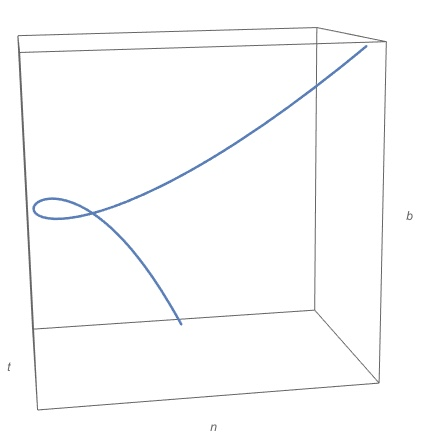
\includegraphics[scale=0.25]{figures_mvc/local_canonical_form}
	\end{center}
	\caption{Trace of a regular space curve in the neighborhood of a point with non-zero curvature and torsion.}
\end{figure}

\begin{figure}[h]
\centering
\begin{subfigure}{.5\textwidth}
  \centering
  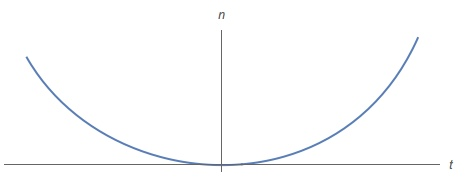
\includegraphics[width=.8\linewidth]{figures_mvc/tn_projection}
  \caption{Projection onto the osculating plane.}
  \label{fig:sub1}
\end{subfigure}%
\begin{subfigure}{.5\textwidth}
  \centering
  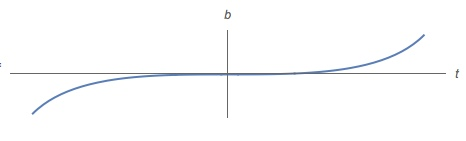
\includegraphics[width=.8\linewidth]{figures_mvc/tb_projection}
  \caption{Projection onto the rectifying plane.}
  \label{fig:sub2}
\end{subfigure}
\begin{subfigure}{.5\textwidth}
  \centering
  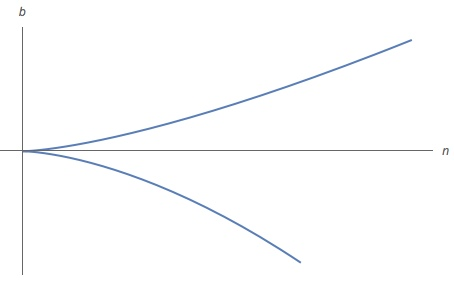
\includegraphics[width=.8\linewidth]{figures_mvc/bn_projection}
  \caption{Projection onto the normal plane.}
  \label{fig:sub3}
\end{subfigure}
\caption{Projections of a regular space curve in the neighborhood of a point with non-zero curvature and torsion onto the osculating, rectifying, and normal planes.}
\label{fig:test}
\end{figure}

Since $\kappa(s)>0$, the Taylor polynomial for $z(h)$ implies that if $\tau(s)>0$, then $z(h)>0$ for sufficiently small positive $h$. On the other hand, if $\tau(s)<0$, then $z(h)<0$ for sufficiently small positive $h$. Thus \emph{positive torsion} at $s$ implies that the the curve $\bbr$ is passing through the osculating plane at $s$ from below. Negative torsion implies from above. Here ``above" means the direction of $\ub(s)$.

\begin{figure}[h]
	\begin{center}
		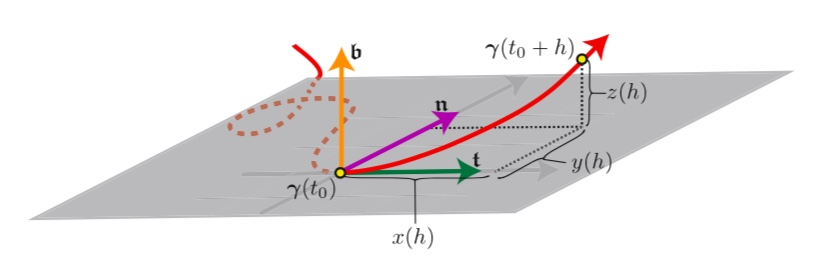
\includegraphics[scale=0.4]{figures_mvc/positive_torsion}
	\end{center}
	\caption{Positive torsion implies that the curve passes through the osculating plane from below.}
\end{figure}

To avoid taking the derivative of the cross product, here is another formula for the torsion which is often more computationally useful.

\begin{prop}
	Let $\bbr:I \to \mathbb{R}^3$ be a regular space curve with an arbitrary parametrization. Then for every $t \in I$ with $\kappa(t) \neq 0$, the torsion is given by
	\begin{align}\label{eq:torsion_jerk}
		\tau(t)=\frac{\bv(t) \times \ba(t)\cdot \bj(t)}{||\bv(t) \times \ba(t)||^2}.
	\end{align}
\end{prop}

\begin{proof}
	We will prove that this formula holds for a curve parametrized by arc length, and that it is also independent of parametrization, which then implies it holds for a curve with any parametrization.
	
	For a curve parametrized by arc length, $\bbr'(s)=\ut(s)$ and $\bbr''(s)=\kappa(s)\un(s)$, and therefore $\bbr'(s) \times \bbr''(s)=\kappa(s)(\ut(s) \times \un(s))=\kappa(s)\ub(s)$ and $||\bbr'(s) \times \bbr''(s)||=||\kappa(s)\ub(s)||=\kappa(s)$. Plugging into \eqref{eq:torsion_jerk}, we have
	\begin{align*}
		\tau(s)&=\frac{\ub(s) \cdot \bbr'''(s)}{\kappa(s)} \\
		&=\frac{\ub(s) \cdot (\kappa(s) \un(s))'}{\kappa(s)} \\
		&=\frac{\kappa'(s) \ub(s)\cdot \un(s)+\kappa(s)\ub(s)\cdot\un'(s)}{\kappa(s)} \\
		&=\frac{\kappa'(s) \cdot 0+\kappa(s)\ub(s)\cdot\un'(s)}{\kappa(s)} \\
		&=\ub(s) \cdot \un'(s) \\
		&=-\ub'(s) \cdot \un(s)
	\end{align*}
in agreement with Definition \ref{def:torsion_for_unit_speed_curve}.

To check that this formula is independent of parametrization, as we computed previously, if $\widetilde{\bbr}=\bbr \circ \varphi$, then
\begin{align*}
	\widetilde{\bv}(t)&=\varphi'(t)\bv(\varphi(t)) \\
	\widetilde{\ba}(t)&=\varphi''(t)\bv(\varphi(t))+(\varphi'(t))^2\ba(\varphi(t)) \\
	\widetilde{\bj}(t)&=\varphi'''(t)\bv(\varphi(t))+3\varphi'(t)\varphi''(t)\ba(\varphi(t))+(\varphi'(t))^3\bj(\varphi(t)).
\end{align*}
Then 
\begin{align*}
	\widetilde{\bv}(t)\times \widetilde{\ba}(t)&=\varphi'(t)\bv(\varphi(t))  \times [\varphi''(t)\bv(\varphi(t))+(\varphi'(t))^2\ba(\varphi(t))] \\
	&=\varphi'(t)\varphi''(t)\underbrace{\bv(\varphi(t))\times \bv(\varphi(t))}_{=0}+(\varphi'(t))^3(\bv(\varphi(t)) \times \ba(\varphi(t))) \\
	&=(\varphi'(t))^3(\bv(\varphi(t)) \times \ba(\varphi(t))) \\
\end{align*}
and therefore
\begin{align*}
	\widetilde{\tau}(t)&=\frac{(\varphi'(t))^3 (\bv(\varphi(t)) \times \ba(\varphi(t)))\cdot (\varphi'''(t)\bv(\varphi(t))+3\varphi'(t)\varphi''(t)\ba(\varphi(t))+(\varphi'(t))^3\bj(\varphi(t)))}{(\varphi'(t))^6||\bbr'(\varphi(t)) \times \ba(\varphi(t))||^2}
\end{align*}
Using the cyclic property of the triple product \footnote{See Proposition 3.33 in my linear algebra notes}, we have 
\begin{align*}
	\bv(t) \times \ba(t) \cdot \bv(t)=\underbrace{\bv(t) \times \bv(t)}_{=0} \cdot \ba(t)  =0
\end{align*}
and 
\begin{align*}
	\bv(t) \times \ba(t) \cdot \ba(t) =\underbrace{\ba(t) \times \ba(t)}_{=0} \cdot \bv(t) =0
\end{align*}
so the formula becomes
\begin{align*}
	\widetilde{\tau}(t)&=\frac{(\varphi'(t))^6 (\bv(\varphi(t)) \times \ba(\varphi(t)))\cdot \bj(\varphi(t)))}{(\varphi'(t))^6||\bv(\varphi(t)) \times \ba(\varphi(t))||^2}\\
	&=\frac{(\bv(\varphi(t)) \times \ba(\varphi(t)))\cdot \bj(\varphi(t)))}{||\bv(\varphi(t)) \times \ba(\varphi(t))||^2} \\
	&=\tau(\varphi(t)) \\
\end{align*}
which shows $\tau$ is invariant under reparametrizations.
\end{proof}

\begin{example}
Consider the twisted cubic $\bbr(t)=(t,t^2,t^3)$ of Example	\ref{ex:twisted_cubic}. The unit binormal vector is given by 

\begin{figure}[h]
	\begin{center}
		\includegraphics[scale=0.5]{figures_mvc/tc_unit_binormal}
	\end{center}
\end{figure}

The torsion function is

\begin{figure}[h]
	\begin{center}
		\includegraphics[scale=0.5]{figures_mvc/tc_torsion_function}
	\end{center}
\end{figure}

Notice that the torsion takes its minimal value of 3 at $t=0$, and then strictly decreases as $|t| \to \infty$.
\end{example}

Physically, we can think of a curve in $\R^3$ a being obtained from a straight line by bending (curvature) and twisting (torsion).

\begin{exercise}
Show that the helix $\bbr(t)=(a\cos t,a\sin t, bt)$ has constant torsion $\tau=\frac{b}{a^2+b^2}$.	
\end{exercise}

\begin{thm}[Fundamental Theorem of the Local Theory of Space Curves]
		Given smooth functions $\kappa(s)>0$ and $\tau(s)$, $s \in I$, there exists a regular parametrized curve $\bbr:I \to \R^3$ such that $s$ is the arc length, $\kappa(s)$ is the curvature, and $\tau(s)$ is the torsion of $\bbr$. This curve is unique up to rotations and translations.
\end{thm}

The proof of this theorem requires differential equations prerequisites, but the theorem says that a space curve is uniquely determined by its curvature and torsion functions. Intuitively, given a straight line, these functions tell you how to obtain the space curve by ``bending" (curvature) and ``twisting" (torsion).

\subsection{Summary of formulas for space curves}
The following formulas hold for arbitrary parametrizations. Here, given a curve $\bbr$,
\begin{align*}
	\bv &\equiv \bbr', \\
	\ba &\equiv \bbr'', \\
	\bj &\equiv \bbr'''. \\
\end{align*}
\begin{enumerate}
	\item Frenet frame
	\begin{align*}
		\ut=\frac{\bv}{||\bv||}, \hspace{0.5cm} \un = \frac{\ut'}{||\ut'||}, \hspace{0.5cm} \ub=\ut \times \un.
	\end{align*}
	\item Curvature function
	\begin{align*}
		\kappa=\frac{||\bv \times \ba||}{||\bv||^3}.
	\end{align*}
	\item Torsion function
	\begin{align*}
		\tau=\frac{\bv \times \ba \cdot {\bf j}}{||\bv \times \ba||^2}.
	\end{align*}
\end{enumerate}

\section{Multivariable Functions}
\subsection{Basic Definitions}
In the last section we studied functions with one input and multiple outputs. In this section, we study functions with multiple input and one output. That is, we study functions of the form
\begin{align*}
	f:U \subseteq \R^n \to \R.
\end{align*}

\begin{example}
\begin{enumerate}[(a)]
	\item The volume of a right circular cylinder of radius $r$ and height $h$ is a function $V:U \subseteq \R^2 \to \R$ defined by $V(r,h)=\pi r^2h$.
	\item The distance function on $\R^n$ is a function $\rho:\R^n \to \R$ defined by
	\begin{align*}
	\rho(x_1,x_2,\dots,x_n)=\sqrt{x_1^2+x_2^2+\cdots+x_n^2}.
	\end{align*}
	\item The ideal gas law is a function giving the pressure in terms of the temperature and volume:
	\begin{align*} 
		p:\R^2 &\to \R\\
		p(T,V)&=\frac{nRT}{V}.
	\end{align*}
\end{enumerate}	
\end{example}
In calculus, one generally defines a function by writing $y=f(x)$, where it is understood that the domain of the function is the largest set for which it is defined. This is common practice for multivariable functions as well, and one writes $z=f(x,y)$ meaning that the value of the function $f$ at $(x,y) \in \R^2$ is $z$. Similarly, one writes $u=f(x,y,z)$, $w=f(x,y,z,u)$, etc., if $f$ depends on more variables.

\begin{example}\label{ex:parab_blue}
Consider the function $f:D \subseteq \R^2 \to \R$ defined by $f(x,y)=\sqrt{y-x^2}$. For the square root to be defined, we must have $y-x^2\geq 0$. Taking the domain $D$ to be the largest set where the function is defined, we have then $D=\{(x,y) \in \R^2:y \geq x^2\}$, which is the shaded region above (and including) the parabola $y=x^2$ shown below. Note that $D$ is closed (since it contains its boundary $y=x^2$) and unbounded. (See Section \ref{sec:regions} for definitions of these terms.)
\begin{figure}[h]
	\begin{center}
		\includegraphics[scale=0.5]{figures_mvc/domain_parab}
	\end{center}
	\caption{The domain of the function $z=\sqrt{y-x^2}$.}
\end{figure}
\end{example}

\begin{exercise}\label{exer:green_circ}
Describe the domain $D$ of the function $f:D \subseteq \R^2 \to \R$ defined by 
\begin{align*}
	f(x,y)=\frac{1}{\sqrt{16-x^2-y^2}}.
\end{align*}	
\end{exercise}

{\color{red}
\begin{solution}
	For the square root to be defined, we must have $16 \geq x^2+y^2$. However, we cannot take $16=x^2+y^2$ since then we divide by zero. Therefore
	\begin{align*}
		D=\{(x,y):x^2+y^2<16\}=B_4(0)
	\end{align*}
	is the open ball of radius 4 centered at $(0,0)$. Note that $D$ is open and bounded.
	\begin{figure}[h]
		\begin{center}
			\includegraphics[scale=0.3]{figures_mvc/dom_ball_4}
		\end{center}
		\caption{The domain of the function $z=\frac{1}{\sqrt{16-x^2-y^2}}$}.
	\end{figure}
\end{solution}}

\begin{exercise}
For each of the following functions, evaluate $f(3,2)$ and find and sketch the domain.
\begin{enumerate}
	\item $f(x,y)=\frac{\sqrt{x+y+1}}{x-1}$
	\item $f(x,y)=x\ln(y^2-x)$
\end{enumerate} 	
\end{exercise}

\begin{figure}[h]
	\begin{center}
	\includegraphics[scale=0.5]{figures_mvc/dom_range_solution}
\end{center}
\end{figure}

\begin{figure}[h]
	\begin{center}
	\includegraphics[scale=0.5]{figures_mvc/dom_range_solution_part_2}
\end{center}
\end{figure}

\subsection{Regions in $\R^n$}\label{sec:regions}
In the study of single-variable functions, open and closed intervals played important roles. We now describe regions of $\R^n$ which are the generalizations of such intervals to higher dimensions.

Most of what follows depends only on the basic properties of the distance function
\begin{align*}
	||\bx-\by||=\sqrt{\sum_{i=1}^n(x_i-y_i)^2}, \hspace{0.5cm} \bx, \by \in \R^n,
\end{align*}
which are exactly the same properties as those of the absolute value function $|x|$, $x \in \R$ (which is the distance function on $\R^n$ for $n=1$).

\begin{thm}[Properties of the distance function]\label{thm:props_of_the_distance_function}
	\begin{enumerate}[(i)]\hspace{15cm}
		\item $||\bx-\by||\geq 0$, with equality if and only if $\bx=\by$;
		\item $||\bx-\by||=||\by-\bx||$;
		\item $||\bx-\by||\leq ||\bx-\bz||+||\bz-\by||$ (triangle inequality).
	\end{enumerate}
\end{thm}

\begin{proof}
Properties (i) and (ii) are obvious from the definition. We prove (iii):

Let $\bu, \bv \in \R^n$. Then
\begin{align*}
	||\bu+\bv||^2&=(\bu+\bv)\cdot (\bu+\bv) \\
	&=||\bu||^2+||\bv||^2+2\bu \cdot \bv \\
	&\leq ||\bu||^2+||\bv||^2+2|\bu \cdot \bv| \\
	&\leq ||\bu||^2+||\bv||^2+2||\bu|| \cdot ||\bv|| \text{ (by the Cauchy-Schwarz inequality)} \\
	&=(||\bu||+||\bv||)^2.
\end{align*}	
Since $||\bu+\bv||$ and $||\bu||+||\bv||$ are nonnegative, it follows that
\begin{align*}
	||\bu+\bv|| \leq ||\bu||+||\bv||.
\end{align*}
The proof of the theorem then follows by taking $\bu=\bx-\bz$ and $\bv=\bz-\by$.
\end{proof}

\begin{defn}[Open Ball]
	Let $\bx_0 \in \R^n$ and let $r>0$. The \emph{open ball of radius $r$ centered at $\bx_0$ is the set}	
	\begin{align*}
		B_r(\bx_0)=\{ \bx \in \R^n:||\bx-\bx_0||<r \}.
	\end{align*}	
\end{defn}

\begin{example}\hspace{15cm}
	\begin{enumerate}[(a)]
		\item In $\R$, the open ball $B_r(x_0)$ is the open interval $(x_0-r,x_0+r)$.
		\item In $\R^2$, the open ball $B_r(\bx_0)$ is the open disc
		\begin{align*}
			B_r(\bx_0)=\{(x,y) \in \R^2:\sqrt{(x-x_0)^2+(y-y_0)^2}<r\}.
		\end{align*}
	\end{enumerate}
\end{example}

\begin{defn}[Interior and boundary]
	Let $U \subset \R^n$ and let $\bx_0 \in U$.
	\begin{enumerate}[(1)]
		\item The point $\bx_0$ is an \emph{interior point} of $U$ if there exists $r>0$ such that $B_r(\bx_0) \subseteq U$. That is, if there exists an open ball centered at $\bx_0$ contained entirely in $U$. The \emph{interior} of $U$, denoted $\text{Int }U$, is the set of interior points of $U$.
		\item The point $\bx_0$ is a \emph{boundary point} of $U$ if for every $r>0$, $B_r(\bx_0)$ contains a point of $U$ as well as a point of $\R^n-U$. The boundary itself need not belong to $U$. The \emph{boundary} of $U$, denoted $\partial U$, is the set of boundary points of $U$.
	\end{enumerate}
\end{defn}

\begin{figure}[h]
	\begin{center}
		\includegraphics[scale=0.5]{figures_mvc/int_bdry}
	\end{center}
	\caption{Interior and boundary points.}
\end{figure}


\begin{defn}[Open and closed sets]\hspace{15cm}
	\begin{enumerate}[(1)]
		\item A subset $U \subseteq \R^n$ is \emph{open} if it consists entirely of interior points.
		\item A subset $U \subseteq \R^n$ is \emph{closed} if it contains all of its boundary points.
	\end{enumerate}
\end{defn}

\begin{figure}[h]
	\begin{center}
		\includegraphics[scale=0.5]{figures_mvc/circ_bdry}
	\end{center}
	\caption{The boundary of the unit disc centered at the origin is the unit circle.}
\end{figure}

\begin{defn}[Neighborhood]
If $A$ is an open set containing a point $\bx$, we say that $A$ is a \emph{neighborhood} of $\bx$.	
\end{defn}


It is immediate from Definition \ref{def:open_set} that $\R^n$ itself and $\emptyset$ are open sets. Here is a nontrivial example:

\newpage 

\begin{prop}\label{prop:open_ball_is_open}
An open ball is an open set.	
\end{prop}

\begin{proof}
	Let $\bx \in B_r(\bx_0)$. Then $h\equiv r-||\bx-\bx_0||>0$. Let $\by \in B_h(\bx)$. Then $||\by-\bx||<h$. It then follows from the triangle inequality that
	\begin{align*}
		||\bx_0-\by|| &\leq ||\bx_0-\bx||+||\bx-\by|| \\
		&<r-h+h=r,
	\end{align*}
	which shows that $\by \in B_r(\bx_0)$, and therefore $B_h(\bx) \subseteq B_r(\bx_0)$. Thus, $B_r(\bx_0)$ is open.
\end{proof}

\begin{figure}[h]
	\begin{center}
		\includegraphics[scale=0.5]{figures_mvc/Openballisopen}
	\end{center}
	\caption{An open ball in $\R^n$ is an open set.}
\end{figure}

Note that a set can be neither open nor closed, or can be both open and closed.

\begin{example}
\begin{enumerate}[(a)]
	\item $\R^n$ is open since every point can be surrounded by an open ball in $\R^n$. Since $\R^n$ has no boundary, it trivially contains all of its boundary points. Hence, $\R^n$ is also closed.
	\item $(0,1] \subset \R$ has boundary $\{0,1\}$. It is not closed since it does not contain 0. It is not open, since any open ball centered at 1 contains points in the complement of $(0,1]$. Hence, $(0,1]$ is neither open nor closed.
\end{enumerate}	
\end{example}

\begin{defn}[Bounded set]
	A subset $U \subseteq \R^n$ is \emph{bounded} if it is contained in some ball of finite radius. If $U$ is not bounded, we say it is \emph{unbounded}.
\end{defn}

\begin{example}
\begin{enumerate}[(a)]
	\item An open ball is bounded.
	\item A line is unbounded.
\end{enumerate}	
\end{example}

\begin{exercise}
Describe the domain $U$ of the function in Example	\ref{ex:parab_blue}.
\end{exercise}

{\color{red}
\begin{solution}
	It is closed (since it contains its boundary $y=x^2$) an unbounded. 
\end{solution}}

\begin{exercise}
Describe the domain $U$ of the function in Example	\ref{exer:green_circ}.
\end{exercise}

{\color{red}
\begin{solution}
	It is open and bounded. 
\end{solution}}

\subsection{Visualizing Multivariable Functions}
\subsubsection{Shapes and Functions}
Consider the following three expressions:
\begin{align*}
	&(\cos(t),\sin(t)) \\
	&x^2+y^2=1 \\
	&\sqrt{1-x^2}
\end{align*}
Each evokes a shape: a circle. (The last may evoke only an arc of a circle.) Let us describe each of these evocations in the language of sets and functions: for each, we define sets $X,Y$, a function $f:X \to Y$, and tell how the shape appears as a subset of either $Y,X,$ or $X \times Y$.

\begin{itemize}
	\item \emph{Image}. As in the previous section, take $X=[0,2\pi)$, $Y=\R^2$, and define
	\begin{align*}
		f:[0,2\pi) &\to \R^2 \\
		t &\mapsto (\cos(t),\sin(t)).
	\end{align*}
	Then the circle is the \emph{image} $f(\R) \subseteq Y$ of the function $f$, a subset of the codomain. The image construction parametrizes a shape.
	\item \emph{Preimage}. Now take $X=\R^2$, $Y=\R$ and define
	\begin{align*}
		f:\R^2 &\to \R, \\
		(x,y) &\mapsto x^2+y^2. 
	\end{align*}
	Then the circle is the \emph{preimage} $f^{-1}(1) \subseteq X$, a subset of the domain.
	\item \emph{Graph}. Take $X=(-1,1)$ and $Y=\R$. Define
	\begin{align*}
		f:[-1,1] &\to \R \\
		x &\mapsto \sqrt{1-x^2}.
	\end{align*}
	Then a half-circle is the graph $\Gamma(f) \subseteq X \times Y$, the subset of the Cartesian product defined by
	\begin{align*}
		\Gamma(f)=\{(x,f(x)): x \in X\}.
	\end{align*}
\end{itemize}

\subsubsection{Visualizing Multivariable Functions}
\begin{defn}
	Let $f:U \subset \mathbb{R}^2 \to \mathbb{R}$ be a real-valued function of two variables.  
\begin{enumerate}[(1)]
	\item The \emph{graph} of $f$ is the set $$\Gamma(f)=\{(x,y,z) \subset \mathbb{R}^3:z=f(x,y)\}$$.
	\item A \emph{level curve} of $f$ is the set
	$$L(f)=\{(x,y) \in U \subset \mathbb{R}^2:f(x,y)=\text{constant}\}$$
	\item To each level curve in the domain we associate a \emph{contour line}, which is the intersection of the plane $z=c$ with the surface $z=f(x,y)$. \\
\end{enumerate}
\end{defn}

\begin{figure}[h]
\centering
\begin{subfigure}{.5\textwidth}
  \centering
  \includegraphics[width=\linewidth]{figures_mvc/graph_def}
\end{subfigure}%
\begin{subfigure}{.5\textwidth}
  \centering
  \includegraphics[width=\linewidth]{figures_mvc/contour_lines_example}
\end{subfigure}
\caption{The graph of a function $z=f(x,y)$ is shown on the left. On the right, contour lines are shown in the domain which are the projections onto the $xy$-plane of the contour lines on the graph.}
\end{figure}

\newpage
\begin{example}
The graph of the function $z=100-x^2-y^2$ is shown below, along with the contour line at $z=75$, and the corresponding level curve.
\begin{figure}[h]
	\begin{center}
	\includegraphics[scale=0.5]{figures_mvc/contour}
\end{center}
\caption{Graph of $z=100-x^2-y^2$. The contour line at $z=75$ and corresponding level curve are shown.}
\end{figure}
	
\end{example}
\begin{example}[Elevation maps]
	On maps, contour lines (really level curves; many people use these terms interchangibly) represent constant elevation.
	\begin{figure}[h]
		\begin{center}
		\includegraphics[scale=0.4]{figures_mvc/mt_greylock}
	\end{center}
	\end{figure}
\end{example}
\newpage 
\begin{example}
Consider the function $f:\mathbb{R}^2 \to \mathbb{R}$ defined by $f(x,y)=y^2$. For any fixed value $x_0$ of $x$, a cross section of the graph is the parabola $z=y^2$ in the $zy$ plane at $x_0$. Since $f(x,y)$ is independent of $x$, the graph has a translational symmetry in the $x$ direction. The graph and level curves can be plotted in \emph{Mathematica} using the commands shown below.

	\begin{figure}[h]
\centering
\begin{subfigure}{.5\textwidth}
  \centering
  \includegraphics[width=\linewidth]{figures_mvc/half_pipe_ex}
  \caption{The graph of the function $z=y^2$.}
\end{subfigure}%
\begin{subfigure}{.5\textwidth}
  \centering
  \includegraphics[width=\linewidth]{figures_mvc/half_pipe_contour}
  \caption{Level curves of the function $z=y^2$.}
\end{subfigure}
\caption{The graph and level curves of the function $z=y^2$.}
\end{figure}
\end{example}

\begin{exercise}
Sketch the graph and level curves of the function $f:\mathbb{R}^2 \to \mathbb{R}$ defined by $f(x,y)=x^2+y^2$. 	
\end{exercise}

{\color{red}
\begin{solution}
\end{solution}}
		\begin{figure}[h]
\centering
\begin{subfigure}{.5\textwidth}
  \centering
  \includegraphics[width=\linewidth]{figures_mvc/paraboloid}
  \caption{The graph of the function $z=x^2+y^2$.}
\end{subfigure}%
\begin{subfigure}{.5\textwidth}
  \centering
  \includegraphics[width=\linewidth]{figures_mvc/paraboloid_contour}
  \caption{Level curves of the function $z=x^2+y^2$.}
\end{subfigure}
\caption{The graph and level curves of the function $z=x^2+y^2$.}
\end{figure}
\newpage 
If $f:U \subset \mathbb{R}^3 \to \mathbb{R}$ is a function of three variables, its graph $\{(x,y,z,f(x,y,z)\}$ is a subset of $\mathbb{R}^4$, and therefore is impossible to visualize. Instead, we visualize the function by its three-dimensional \emph{level surfaces}.

\begin{defn}[Level surfaces]
A \emph{level surface} of $f$ is the set
\begin{align*}
	L(f)=\{(x,y,z) \in U \subset \mathbb{R}^3:f(x,y,z)=\text{constant}\}
\end{align*}	
\end{defn}
\begin{example}
The level surfaces of the function $f:\R^3 \to \R$ defined by $f(x,y,z)=x^2+y^2+z^2$ are concentric spheres. These can be plotted in \emph{Mathematica} using the command shown below:
\begin{figure}[h]
	\begin{center}
		\includegraphics[scale=0.4]{figures_mvc/concentric_spheres_contour}
	\end{center}
	\caption{Level surfaces of $f(x,y,z)=x^2+y^2+z^2$.}
\end{figure}
\end{example}
\newpage 
\begin{exercise}
Plot the level surfaces of the function $f:\R^3 \to \R$ defined by $f(x,y,z)=z$.	
\end{exercise}

{\color{red}
\begin{solution}
	\begin{figure}[h]
	\begin{center}
		\includegraphics[scale=0.4]{figures_mvc/planes_level}
	\end{center}
	\caption{Level surfaces of $f(x,y,z)=z$.}
\end{figure}
\end{solution}}

\begin{exercise}
Plot the level surfaces of the function $f:\R^3 \to \R$ defined by $f(x,y,z)=x+z$.	
\end{exercise}
{\color{red}
\begin{solution}
	\begin{figure}[h]
	\begin{center}
		\includegraphics[scale=0.4]{figures_mvc/level_surf_x_p_z}
	\end{center}
	\caption{Level surfaces of $f(x,y,z)=x+z$.}
\end{figure}
\end{solution}}

\subsection{Quadric Surfaces}
\begin{defn}[Quadric Surface]
	Let $A,B,C,D,E,F,G,H,I,J,K$ be fixed real numbers and define a function
	\begin{align*}
		f:\R^3 &\to \R  \\
		(x,y,z)&\mapsto Ax^2+By^2+Cz^2+Dxy+Eyz+Fxz+Gx+Hy+Jz+K.
	\end{align*}
	A \emph{quadric surface} is the preimage $f^{-1}(0)$; that is, it is the set of all points $(x,y,z) \in \R^3$ such that 
	\begin{align*}
		Ax^2+By^2+Cz^2+Dxy+Eyz+Fxz+Gx+Hy+Jz+K=0.
	\end{align*}
\end{defn}
Here, we will consider some famous quadric surfaces and plot them in \emph{Mathematica}. Many examples of functions of two variables in this unit will have these quadric surfaces as graphs.

\subsubsection{Ellipsoids}
\begin{defn}[Ellipsoid]
	An \emph{ellipsoid} is the quadric surface whose equation is of the form
	\begin{align*}
		\frac{x^2}{a^2}+\frac{y^2}{b^2}+\frac{z^2}{c^2}=1.
	\end{align*}
\end{defn}
Note that the intersection of this surface with each coordinate plane is an ellipse. For example,
\begin{align*}
	\frac{x^2}{a^2}+\frac{y^2}{b^2}=1 \hspace{0.5cm} \text{ when } z=0.
\end{align*}
If any two of the parameters $a,b,c$ are equal, then the surface is an \emph{ellipsoid of revolution}. If all three are equal, the surface is a sphere.
\begin{figure}[h]
	\begin{center}
		\includegraphics[scale=0.4]{figures_mvc/mma_ellipsoid}
	\end{center}
	\caption{The ellipsoid $\frac{x^2}{4}+\frac{y^2}{9}+\frac{z^2}{16}=1$.}
\end{figure}

\subsubsection{Paraboloids}
\begin{defn}[Elliptic Paraboloid]
	An \emph{elliptic paraboloid} is the quadric described by the equation
	\begin{align*}
		\frac{x^2}{a^2}+\frac{y^2}{b^2}=\frac{z}{c}.
	\end{align*}
\end{defn}
Except for the point $(0,0,0)$, the surface lies entirely above or entirely below the $xy$-plane, depending on the sign of $c$.

\begin{figure}[h]
\centering
\begin{subfigure}{.5\textwidth}
  \centering
  \includegraphics[width=\linewidth]{figures_mvc/el_paraboloid_1}
  \caption{The elliptic paraboloid $\frac{x^2}{4}+\frac{y^2}{9}=\frac{z}{16}$.}
\end{subfigure}%
\begin{subfigure}{.5\textwidth}
  \centering
  \includegraphics[width=\linewidth]{figures_mvc/el_paraboloid_2}
  \caption{The elliptic paraboloid $\frac{x^2}{4}+\frac{y^2}{9}=-\frac{z}{16}$.}
\end{subfigure}
\end{figure}
The intersections of the surface with the coordinate planes are
\begin{align*}
	&x=0: \text{ the parabola } z=\frac{c}{b^2}y^2 \\
	&y=0: \text{ the parabola } z=\frac{c}{a^2}x^2 \\
	&z=0: \text{ the point } (0,0,0). \\
\end{align*}

Each plane $z=z_0$ above the $xy$-plane intersects the surface in the ellipse
\begin{align*}
	\frac{x^2}{a^2}+\frac{y^2}{b^2}=\frac{z_0}{c}.
\end{align*}
If $a=b$, the surface is called a \emph{circular paraboloid} or a \emph{paraboloid of revolution}.

\subsubsection{Cones}
\begin{defn}[Cone]
	An \emph{elliptic cone} is the quadric surface described by the equation
	\begin{align*}
		\frac{x^2}{a^2}+\frac{y^2}{b^2}=\frac{z^2}{c^2}.
	\end{align*}
\end{defn}

\begin{figure}[h]
	\begin{center}
		\includegraphics[scale=0.5]{figures_mvc/cone}
	\end{center}
	\caption{A cone.}
\end{figure}

The intersections of the surface with the coordinate planes are
\begin{align*}
	&x=0: \text{ the lines } z=\pm \frac{c}{b}y \\
	&y=0: \text{ the parabola } z=\pm \frac{c}{a}x \\
	&z=0: \text{ the point } (0,0,0). \\
\end{align*}
The intersections with the planes $z=z_0$ above and below the $xy$-plane are ellipses whose centers lie on the $z$-axis and whose vertices lie on the above lines. 

If $a=b$, the cone is a \emph{right circular cone}.

\subsubsection{Hyperboloids}
\begin{defn}[Hyperboloid of one sheet]
	A \emph{hyperboloid of one sheet} is the quadric surface described by the equation
	\begin{align*}
		\frac{x^2}{a^2}+\frac{y^2}{b^2}-\frac{z^2}{c^2}=1.
	\end{align*}
\end{defn}

\begin{figure}[h]
	\begin{center}
		\includegraphics[scale=0.5]{figures_mvc/hyp_1_sheet}
	\end{center}
	\caption{A hyperboloid of one sheet.}
\end{figure}

The intersections with the coordinate planes are
\begin{align*}
	&x=0: \text{ the hyperbola } \frac{y^2}{b^2}-\frac{z^2}{c^2}=1 \\
	&y=0: \text{ the hyperbola } \frac{x^2}{a^2}-\frac{z^2}{c^2}=1 \\
	&z=0: \text{ the ellipse } \frac{x^2}{a^2}+\frac{y^2}{b^2}=1. \\
\end{align*}
The plane $z=z_0$ intersects the surface in an ellipse with center on the $z$-axis and vertices on one of the above hyperbolas.

The surface is connected, meaning that it is possible to travel from one point on it to any other without leaving the surface. For this reason, it is said to have \emph{one sheet}, in contrast to the hyperboloid in the next example, which has two sheets.

If $a=b$, the hyperboloid is a surface of revolution. 

\begin{defn}[Hyperboloid of two sheets]
	A \emph{hyperboloid of two sheets} is the quadric surface described by the equation
	\begin{align*}
		-\frac{x^2}{a^2}-\frac{y^2}{b^2}+\frac{z^2}{c^2}=1.
	\end{align*}
\end{defn}

\begin{figure}[h]
	\begin{center}
		\includegraphics[scale=0.5]{figures_mvc/hyp_2_sheets}
	\end{center}
	\caption{A hyperboloid of two sheets.}
\end{figure}

The plane $z=0$ does not intersect the surface; in fact, for a horizontal plane to intersect the surface, we must have $|z|\geq |c|$. The hyperbolic cross-sections 
\begin{align*}
	&x=0: \frac{z^2}{c^2}-\frac{y^2}{b^2}=1 \\
	&y=0: \frac{z^2}{c^2}-\frac{x^2}{a^2}=1 \\
\end{align*}
have their vertices and foci on the $z$-axis. The surface has two disconnected components, one above the plane $z=c$ and the other below the plane $z=-c$.

\subsubsection{Hyperbolic Paraboloids}
\begin{defn}[Hyperbolic paraboloid]
	A \emph{hyperbolic paraboloid} is the quadric surface described by the equation
	\begin{align*}
		\frac{y^2}{b^2}-\frac{x^2}{a^2}=\frac{z}{c}, \hspace{0.5cm} c>0.
	\end{align*}
\end{defn}
\begin{figure}[h]
	\begin{center}
		\includegraphics[scale=0.5]{figures_mvc/last_one}
	\end{center}
	\caption{A hyperbolic paraboloid.}
\end{figure}
The intersections with the coordinate planes are
\begin{align*}
	&x=0: \text{ the parabola } z=\frac{c}{b^2}y^2 \\
	&y=0: \text{ the parabola } z=-\frac{c}{a^2}x^2. 
\end{align*}
In the plane $x=0$, the parabola opens upward from the origin. The parabola in the plane $y=0$ opens downward.

The intersection of the surface with a plane $z=z_0>0$ is the hyperbola
\begin{align*}
	\frac{y^2}{b^2}-\frac{x^2}{a^2}=\frac{z_0}{c}.
\end{align*}

Near the origin, the surface is shaped like a saddle. To a person traveling along the surface in the $yz$-plane, the origin looks like a minimum. To a person traveling in the $xz$-plane, the origin looks like a maximum. Such a point is called a \emph{saddle point} of a surface.

\begin{exercise}
Work out the various cross-sections of the quadric surfaces described above and verify the claims in this section.	
\end{exercise}

\newpage 

\subsection{Limits}
Let's compare the behavior of the functions
\begin{align*}
	f(x,y)=\frac{\sin{(x^2+y^2)}}{x^2+y^2} \hspace{0.5cm} \text{ and } \hspace{0.5cm} g(x,y)=\frac{x^2-y^2}{x^2+y^2}
\end{align*}
as $(x,y) \to (0,0)$. Note that neither function is defined at $(0,0)$:

\begin{figure}[h]
\begin{center}
\includegraphics[scale=0.5]{figures_mvc/tables_f_g}
\end{center}	
\end{figure}
It looks like $\lim_{(x,y) \to (0,0)}f(x,y)=1$ (since the values of the function approach 1 from all directions) while $\lim_{(x,y) \to (0,0)}g(x,y)$ does not exist (since the values of the function near $(0,0)$ do not approach any fixed value).

\begin{defn}[Limit]\label{def:limit}
Let $U$ be an open subset of $\R^n$ and $f:U \to \mathbb{R}$, which may or may not be defined at $\bx_0 \in U$, and let $L \in \mathbb{R}$. We say that 
\begin{align*}
	\lim_{\bx \to \bx_0}f(\bx)=L
\end{align*}
if for every $\epsilon > 0$ there exists a corresponding $\delta>0$ such that
\begin{align*}
	0<||\bx-\bx_0||<\delta \implies |f(\bx)-L|<\epsilon.
\end{align*}
In this case $L$ is called the \emph{limit} of $f$ as $\bx$ approaches $\bx_0$.
\end{defn}
This definition says that the distance between $f(\bx)$ and $L$ can be made arbitrarily small by making the distance between $\bx$ and  $\bx_0$ sufficiently small. \footnote{Two points $x_1,x_2$ are said to be \emph{arbitrarily close} if, for \emph{every} $\epsilon>0$, $d(x_1,x_2)<\epsilon$. A point $x_1$ is said to be \emph{sufficiently close} to $x_2$ if there exists \emph{some} (fixed) $\delta>0$ such that $d(x_1,x_2)<\delta$.}

\begin{figure}[h]
	\begin{center}
	\includegraphics[scale=0.4]{figures_mvc/limit_def}
\end{center}
\caption{A function $f(\bx)$ has limit $L$ as $\bx \to \bx_0$ if $f(\bx)$ can be made arbitrarily close to $L$ by taking $\bx$ sufficiently close to $\bx_0$.}
\end{figure}

\newpage

As in single-variable calculus, another illustration of the definition of a limit can be given in terms of its graph: For any $\epsilon>0$, we can find $\delta>0$ such that if $\bx \in B_\delta(\bx_0)$ and $\bx \neq \bx_0$, then $f(x)$ lies between the horizontal planes $z=L-\epsilon$ and $z=L+\epsilon$.

	\begin{figure}[h]
		\begin{center}
	\includegraphics[scale=0.7]{figures_mvc/limit_def_graph}
	\end{center}
	\caption{A function $f$ has limit $L$ as $\bx \to \bx_0$ if the graph can be bounded between two arbitrarily close planes whenever for all $\bx$ sufficiently close to $\bx_0$.}
	\end{figure}
	
For functions of a single variable, when we let $x \to a$, there are only two directions of approach: from the left or from the right. Recall that if $\lim_{x \to a^-}f(x) \neq \lim_{x \to a^+}f(x)$, then $\lim_{x \to a}f(x)$ does not exist. For functions of two variables, we can let $(x,y)$ approach $(a,b)$ from an infinite number of directions, as long as $(x,y)$ stays within the domain of $f$.
	
\begin{figure}[h]
	\begin{center}
		\includegraphics[scale=0.5]{figures_mvc/approach}
	\end{center}
	\caption{Various paths in the domain of a function $f:\R^2 \to \R$ along which we can approach a point $(a,b)$.}
\end{figure}	
	
	
Note that the definition of a limit only depends on the \emph{distance} from $(x,y)$ and $(a,b)$. It does \emph{not} refer to the direction of the approach. Therefore, if the limit exists, then $f(x,y)$ must approach the same limit no matter how $(x,y)$ approaches $(a,b)$. Thus, if we can find two different paths of approach along which the function $f(x,y)$ has different limits, then it follows that $\lim_{(x,y) \to (a,b)}f(x,y)$ does not exist.

\begin{example}
Consider $\lim_{(x,y) \to (0,0)}\frac{x^2-y^2}{x^2+y^2}$. Consider approaching $(0,0)$ along the $x$-axis, that is, along the curve $\bbr(t)=(t,0)$. Then
\begin{align*}
	\lim_{(x(t),y(t)) \to (0,0)}\frac{x(t)^2-y(t)^2}{x(t)^2+y(t)^2}=\lim_{t \to 0}\frac{t^2-0}{t^2+0}=\lim_{t \to 0}\frac{t^2}{t^2}=\lim_{t \to 0}1=1.
\end{align*}
Approaching $(0,0)$ along the $y$-axis, i.e., along the path $\bbr(t)=(0,t)$, we find
	\begin{align*}
	\lim_{(x(t),y(t)) \to (0,0)}\frac{x(t)^2-y(t)^2}{x(t)^2+y(t)^2}=\lim_{t \to 0}\frac{0-t^2}{0+t^2}=\lim_{t \to 0}\frac{-t^2}{t^2}=\lim_{t \to 0}(-1)=-1.
\end{align*}
We have found two paths along which $\lim_{(x,y) \to (0,0)}\frac{x^2-y^2}{x^2+y^2}$ has different values, so $\lim_{(x,y) \to (0,0)}\frac{x^2-y^2}{x^2+y^2}$ does not exist.
\end{example}

\begin{figure}[h]
	\begin{center}
		\includegraphics[scale=0.5]{figures_mvc/no_limit_ex}
	\end{center}
	\caption{The function $f(x,y)=\frac{x^2-y^2}{x^2+y^2}$ has no limit as $(x,y) \to (0,0)$.}
\end{figure}

\begin{example}
	Consider $\lim_{(x,y) \to (0,0)}\frac{xy}{x^2+y^2}$. Approaching $(0,0)$ along the $x$-axis gives
	\begin{align*}
		\lim_{x \to 0} \frac{x \cdot 0}{x^2+0}=\lim_{x \to 0} \frac{0}{x^2}=0.
	\end{align*}
	Approaching $(0,0)$ along the $y$-axis gives
	\begin{align*}
		\lim_{y \to 0} \frac{0 \cdot y}{0+y^2}=\lim_{y \to 0} \frac{0}{y^2}=0.
	\end{align*}
While these limits agree, this is \emph{not} sufficient to conclude that $\lim_{(x,y) \to (0,0)}\frac{xy}{x^2+y^2}=0$, since we must show that we obtain the same limit along \emph{every} path approaching $(0,0)$. Indeed, if we approach $(0,0)$ along the line $y=x$, we obtain
\begin{align*}
	\lim_{x \to 0}\frac{x^2}{x^2+x^2}=\lim_{x \to 0}\frac{x^2}{2x^2}=\lim_{x \to 0}\frac{1}{2}=\frac{1}{2}.
\end{align*}
Thus, $\lim_{(x,y) \to (0,0)}\frac{xy}{x^2+y^2}$ does not exist.
\end{example}

\begin{figure}[h]
	\begin{center}
		\includegraphics[scale=0.5]{figures_mvc/xy_not_suff}
	\end{center}
	\caption{The function $f(x,y)=\frac{xy}{x^2+y^2}$ has no limit as $(x,y) \to (0,0)$.}
\end{figure}
\newpage 
The previous example shows that it is not sufficient to compute the limit of a multivariable function by restricting the function to paths in the domain. We now show how to use Definition \ref{def:limit} to show that a limit \emph{does} exist.

\begin{thm}\label{thm:simple_limits}
Let $a,b,c$ be fixed real numbers. Then
\begin{enumerate}[(a)]
	\item $\lim_{(x,y) \to (a,b)} c=c$.
	\item $\lim_{(x,y) \to (a,b)} x = a$.
	\item $\lim_{(x,y) \to (a,b)} y = b$.
\end{enumerate}	
\end{thm}

\begin{proof}\hspace{15cm}
	\begin{enumerate}[(a)]
		\item Let $\epsilon>0$. Since $|c-c|=0$, by taking $\delta$ to be any positive real number, then \newline $0<\sqrt{(x-a)^2+(y-b)^2}<\delta$ implies $|f(x,y)-f(a,b)|=|c-c|=0<\epsilon$. This proves that $\lim_{(x,y) \to (a,b)} c=c$.
		\item Let $\epsilon>0$. We have $|f(x,y)-f(a,b)|=|x-a|$. Since 
		\begin{align*}
			|x-a|=\sqrt{(x-a)^2} \leq \sqrt{(x-a)^2+(y-b)^2},
		\end{align*}
		by taking $\delta=\epsilon$, $0<\sqrt{(x-a)^2+(y-b)^2}<\delta$ implies that $|f(x,y)-f(a,b)|=|x-a|<\epsilon$. This proves that $\lim_{(x,y) \to (a,b)} x = a$.
		\item The proof is essentially the same as that of part (b) and is left as an exercise.
	\end{enumerate}
\end{proof}

\begin{exercise}
Prove part (c) of Theorem \ref{thm:simple_limits}. 	
\end{exercise}

{\color{red}
\begin{solution}
	Let $\epsilon>0$. We have $|f(x,y)-f(a,b)|=|y-b|$. Since 
		\begin{align*}
			|y-b|=\sqrt{(y-b)^2} \leq \sqrt{(x-a)^2+(y-b)^2},
		\end{align*}
		by taking $\delta=\epsilon$, $0<\sqrt{(x-a)^2+(y-b)^2}<\delta$ implies that $|f(x,y)-f(a,b)|=|y-b|<\epsilon$. This proves that $\lim_{(x,y) \to (a,b)} y = b$.
\end{solution}}

The next theorem shows that all of the limit properties of single-variable functions carry over to multivariable functions.

\begin{thm}[Limit laws for multivariable functions]\label{thm:limit_laws_for_multivariable_functions}
Suppose $f(x,y)$ and $g(x,y)$ are defined on the same open set containing $(x_0,y_0)$, and that 
\begin{align*}
	\lim_{(x,y) \to (x_0,y_0)}f(x,y)=L \hspace{0.5cm} \text{ and } \hspace{0.5cm} \lim_{(x,y) \to (x_0,y_0)}g(x,y)=M.
\end{align*}
Then
	\begin{enumerate}[(i)]
		\item $\lim_{(x,y) \to (x_0,y_0)} cf(x,y)=cL$ for any $c \in \R$;
		\item $\lim_{(x,y) \to (x_0,y_0)}(f(x,y)+ g(x,y))=L+M$;
		\item $\lim_{(x,y) \to (x_0,y_0)}(f(x,y)g(x,y))=LM$;
		\item $\lim_{(x,y) \to (x_0,y_0)}=\frac{f(x,y)}{g(x,y)}=\frac{L}{M}$ whenever $M \neq 0$.
	\end{enumerate}
\end{thm}

\begin{pf}
It follows from Theorem \ref{thm:props_of_the_distance_function} that the proofs of these properties are identical to the proofs of the corresponding properties of single-variable functions in Theorem \ref{thm:limit_laws_for_single-variable_functions}, with the absolute value replaced by the distance function on $\R^n$.
\end{pf}

\begin{example}
To evaluate $\lim_{(x,y) \to (1,2)}(x^2y^3-x^3y^2+3x+2y)$ using Theorems \ref{thm:limit_laws_for_multivariable_functions} and \ref{thm:simple_limits}, we have
\begin{align*}
	&\lim_{(x,y) \to (1,2)}(x^2y^3-x^3y^2+3x+2y)=\lim_{(x,y) \to (1,2)}(x^2y^3)+\lim_{(x,y) \to (1,2)}(-x^3y^2)+\lim_{(x,y) \to (1,2)}(3x+2y) \\
	&=\lim_{(x,y) \to (1,2)}x^2\cdot \lim_{(x,y) \to (1,2)}y^3 - \lim_{(x,y) \to (1,2)} x^3\cdot \lim_{(x,y) \to (1,2)} y^2+3\lim_{(x,y) \to (1,2)} x+2\lim_{(x,y) \to (1,2)}y \\
	&=(\lim_{(x,y) \to (1,2)}x)^2\cdot (\lim_{(x,y) \to (1,2)}y)^3 - (\lim_{(x,y) \to (1,2)} x)^3\cdot (\lim_{(x,y) \to (1,2)} y)^2+3\lim_{(x,y) \to (1,2)} x+2\lim_{(x,y) \to (1,2)}y \\ 
	&=(1)^2(2)^3-(1)^3(2)^2+3(1)+2(2) \\
	&=8-4+3+4 \\
	&=11.
\end{align*} 	
\end{example}

\begin{defn}[Continuous function]
 A multivariable function $f:U \subseteq \R^n \to \R$ is \emph{continuous at} $\bx_0$ if
\begin{align*}
	\lim_{\bx \to \bx_0}f(\bx)=f(\bx_0).
\end{align*}
The function $f$ is \emph{continuous on} $U$ if $f$ is continuous at every point in $U$.	
\end{defn}
As in single-variable calculus, continuous functions map nearby points in $U$ to nearby points in $\mathbb{R}$, so the graph of a continuous function has no holes or breaks.

It follows immediately from Theorem \ref{thm:limit_laws_for_multivariable_functions} that that sums, products, and quotients of continuous functions are continuous on their domains. Similarly, compositions of continuous functions are continuous.  

It follows from Theorem \ref{thm:simple_limits} that $f(x,y)=x, g(x,y)=y,$ and $h(x,y)=c$ are continuous. Since any polynomial, e.g.,
\begin{align*}
	f(x,y)=x^4+5x^3y^2+6xy^4-7y+6
\end{align*}
can be built out of these by multiplication and addition, all polynomials are continuous on $\mathbb{R}^2$. Likewise, any rational function is continuous on its domain because it is a quotient of continuous functions. E.g.,
\begin{align*}
	g(x,y)=\frac{2xy+1}{x^2+y^2}.
\end{align*}

\begin{example}
The function $f(x,y)=\frac{x^2-y^2}{x^2+y^2}$ is continuous everywhere except at $(0,0)$.	
\end{example}

\begin{exercise}
Where is the function
\begin{align*}
	g(x,y)=\begin{cases}
		\frac{x^4-x^2y^2}{x+y}, &\text{ if } (x,y) \neq (0,0), \\
		0, &\text{ if } (x,y)=(0,0).
	\end{cases}
\end{align*}	
continuous?
\end{exercise}

{\color{red}
\begin{solution}
	Since a rational function is continuous everywhere it is defined, $g(x,y)$ is continuous for all $(x,y) \neq (0,0)$. Since for $(x,y) \neq (0,0)$
	\begin{align*}
		\frac{x^4-x^2y^2}{x+y}=\frac{x^2(x^2-y^2)}{x+y}=\frac{x^2(x+y)(x-y)}{x+y}=x^2(x-y),
	\end{align*}
	we have 
	\begin{align*}
		\lim_{(x,y) \to (0,0)}\frac{x^4-x^2y^2}{x+y}=\lim_{(x,y) \to (0,0)}x^2(x-y)=0=g(0,0).
	\end{align*}
	Thus, $g(x,y)$ is continuous everywhere.
\end{solution}}
\newpage

\subsection{Partial Derivatives}
\subsubsection{Motivation}
\begin{example}[Heat index]\hspace{15cm}
\begin{figure}[h]
	\begin{center}
		\includegraphics[width=\textwidth]{figures_mvc/h_i_1}
	\end{center}
\end{figure}
	
\begin{figure}[h]
	\begin{center}
	\includegraphics[scale=0.45]{figures_mvc/heat_index}
	\end{center}
\end{figure}

\begin{figure}[h]
	\begin{center}
		\includegraphics[width=\textwidth]{figures_mvc/h_i_2}
	\end{center}
\end{figure}

\newpage

\begin{figure}[h]
	\begin{center}
		\includegraphics[width=\textwidth]{figures_mvc/h_i_4}
	\end{center}
\end{figure}
By averaging these values we get the estimate $G'(70) \approx 0.9$. This says that, when the temperature is $96^\circ$ F and the relative humidity is $70\%$, the heat index rises about $0.9^\circ$ F for every percent the relative humidity rises.
\end{example} 
In general, if $f(x,y)$ is a function of two variables $x$ and $y$, and we consider the values of the function obtained by varying $x$ (say) while keeping $y$ fixed to a constant value $y=y_0$, then we are really considering a function of a \emph{single} variable $g(x)=f(x,y_0)$. Then if $g(x)$ is differentiable at $x=x_0$, we call $g'(x)$ a \emph{partial derivative} of $f(x,y)$. We now define this formally.

\newpage 
\subsubsection{Definition of Partial Derivatives}
\begin{defn}[Partial derivative]
	Let $f:U \subset \R^2 \to \R$ be defined on an open subset of $\R^2$ containing the point $(x_0,y_0)$. \footnote{Since $U$ is open, there exists a neighborhood of $(x_0,y_0)$ contained in $U$. Thus, if $h$ is sufficiently close to zero, then all points of the form $(x_0+h,y_0)$ will be in $U$, so this definition makes sense.} Then the real number
	\begin{align*}
		\frac{\partial f}{\partial x}(x_0,y_0)&=\lim_{h \to 0}\frac{f(x+h,y)-f(x,y)}{h} \\
	\end{align*}
	is called the \emph{partial derivative of $f$ with respect to $x$ at the point $(x_0,y_0)$}, provided this limit exists. Similarly, the real number
	\begin{align*}
		\frac{\partial f}{\partial y}(x_0,y_0)&=\lim_{h \to 0}\frac{f(x,y+h)-f(x,y)}{h}
	\end{align*}
	is called the \emph{partial derivative of $f$ with respect to $y$ at the point $(x_0,y_0)$}, provided this limit exists. If $\frac{\partial f}{\partial x}$ and $\frac{\partial f}{\partial y}$ are defined at all points of $U$, then they are functions on $U$.
\end{defn}

\begin{remark}
Note that $\frac{\partial f}{\partial x}$ is not a quotient, but a \emph{limit} of a quotient. Thus, the symbols ``$\partial f$" or ``$\partial x$" do not have independent meaning. Similar remarks apply to $\frac{\partial f}{\partial y}$. While this is the most common notation for the partial derivatives (and the one we will use almost exclusively), other notations are also frequently used.
\end{remark}
\begin{figure}[h]
	\begin{center}
	\includegraphics[scale=0.5]{figures_mvc/p_d_notation}
\end{center}
\caption{Notations for partial derivatives.}
\end{figure}
To compute the partial derivative of a function $f(x,y)$ with respect to $x$, one simply treats $y$ as a constant and differentiates $f(x,y)$ with respect to $x$. To compute the partial derivative with respect to $y$, treat $x$ as a constant and differentiate $f(x,y)$ with respect to $y$.

\begin{example}
If $f(x,y)=x^3+x^2y^3-2y^2$, then
\begin{align*}
	\frac{\partial f}{\partial x}&=3x^2+2xy^3 \\
	\frac{\partial f}{\partial y}&=3x^2y^2-4y.
\end{align*}	
\end{example}
\newpage

\subsubsection{Interpretation of Partial Derivatives}

\begin{figure}[h]
	\begin{center}
		\includegraphics[width=\textwidth]{figures_mvc/pd_1}
	\end{center}
\end{figure}

\begin{figure}[h]
	\begin{center}
		\includegraphics[width=\textwidth]{figures_mvc/pd_2}
	\end{center}
\end{figure}

\begin{figure}[h]
	\begin{center}
		\includegraphics[scale=0.5]{figures_mvc/pd_3}
	\end{center}
\end{figure}
\newpage 
\begin{exercise}
If $f(x,y)=\sin\left(\frac{x}{1+y}\right)$, calculate $\frac{\partial f}{\partial x}$ and $\frac{\partial f}{\partial y}$.
\end{exercise}

\begin{figure}[h]
	\begin{center}
		\includegraphics[scale=0.5]{figures_mvc/pd_ex_3_soln}
	\end{center}
\end{figure}

\begin{exercise}
If $f(x,y)=y\sin(xy)$, calculate $\frac{\partial f}{\partial x}$ and $\frac{\partial f}{\partial y}$.	
\end{exercise}

{\color{red}
\begin{solution}
	\begin{align*}
		\frac{\partial f}{\partial x}=y^2\cos(xy), \hspace{0.5cm}
	\frac{\partial f}{\partial y}=\sin(xy)+xy\cos(xy).
	\end{align*}	
\end{solution}}

 \begin{exercise}
If $f(x,y)=\frac{2y}{y+\cos(x)}$, calculate $\frac{\partial f}{\partial x}$ and $\frac{\partial f}{\partial y}$.	
\end{exercise}

{\color{red}\begin{solution}
	\begin{align*}
		\frac{\partial f}{\partial x}=\frac{2y\sin(x)}{(y+\cos(x))^2}, \hspace{0.5cm}
	\frac{\partial f}{\partial y}=\frac{2\cos(x)}{(y+\cos(x))^2}.
	\end{align*}	
\end{solution}}


\subsubsection{Functions of More than Two Variables}
\begin{figure}[h]
	\begin{center}
		\includegraphics[width=\textwidth]{figures_mvc/more_var_pd}
	\end{center}
\end{figure}
That is, we hold all the variables other than $x_i$ constant and differentiate $f$ with respect to $x_i$.

\begin{exercise}
Compute $\frac{\partial f}{\partial x}, \frac{\partial f}{\partial y}$, and  $\frac{\partial f}{\partial z}$ if $f(x,y,z)=e^{xy}\ln z$. 	
\end{exercise}

\begin{figure}[h]
	\begin{center}
		\includegraphics[scale=0.5]{figures_mvc/pd3vex}
	\end{center}
\end{figure}

\subsubsection{Implicit Partial Differentiation}
Implicit partial differentiation works exactly as in the single variable case.

\begin{example}
If the equation
\begin{align*}
	yz-\ln z=x+y
\end{align*}	
defines $z$ implicitly as a function of $x$ and $y$, then we compute $\frac{\partial z}{\partial x}$ by differentiating each side with respect to $x$:
\begin{align*}
	y\frac{\partial z}{\partial x}-\frac{1}{z}\frac{\partial z}{\partial x}&=1 \\
	\implies \frac{\partial z}{\partial x}&=\frac{1}{y-\frac{1}{z}}.
\end{align*}
\end{example}

\begin{exercise}
	Compute $\frac{\partial z}{\partial y}$ if the equation
\begin{align*}
	yz-\ln z=x+y
\end{align*}	
defines $z$ implicitly as a function of $x$ and $y$.
\end{exercise}

{\color{red}
\begin{solution}
\begin{align*}
	\frac{\partial z}{\partial y}=\frac{1-z}{y}.
\end{align*}	
\end{solution}

}



\subsubsection{Higher Partial Derivatives}
\begin{figure}[h]
	\begin{center}
		\includegraphics[width=\textwidth]{figures_mvc/higher_d}
	\end{center}
\end{figure}

\newpage 

\begin{exercise}\label{ex:mixed_partials_equality}
Compute the second partial derivatives of 
\begin{align*}
	f(x,y)=x^3+x^2y^3-2y^2.
\end{align*}	
\end{exercise}

\begin{figure}[h]
	\begin{center}
		\includegraphics[scale=0.5]{figures_mvc/higher_d_ex}
	\end{center}
\end{figure}
Notice for the function in Exercise \ref{ex:mixed_partials_equality} that $\frac{\partial f}{\partial x \partial y}=\frac{\partial f}{\partial y \partial x}$. This is no coincidence.

\begin{thm}[Equality of mixed partial derivatives]\label{thm:clairaut}
Let $f:U \subseteq \R^2 \to \R$. If $\frac{\partial f}{\partial x \partial y}$ and $\frac{\partial f}{\partial y \partial x}$	are both continuous on $U$, then $\frac{\partial f}{\partial x \partial y}=\frac{\partial f}{\partial y \partial x}$ throughout $U$.
\end{thm}

\begin{proof}
	Let $h \neq 0$ and consider the quantity
	\begin{align}\label{eq:clairaut_delta_h}
		\Delta(h)\equiv [f(a+h,b+h)-f(a+h,b)]-[f(a,b+h)-f(a,b)].
	\end{align}
	If we let $g(x) \equiv f(x,b+h)-f(x,b)$, then
	\begin{align*}
		\Delta(h)=g(a+h)-g(a).
	\end{align*}
	If $g$ is differentiable on $U$, by the Mean Value Theorem there exists $c \in (a,a+h)$ such that
	\begin{align*}
		g(a+h)-g(a)&=hg'(c) \\
		&=h\left[\frac{\partial f}{\partial x}(c,b+h)-\frac{\partial f}{\partial x}(c,b)\right].
	\end{align*}
	Applying the Mean Value Theorem again to $\frac{\partial f}{\partial x}$, there exists $d \in (b,b+h)$ such that 
	\begin{align*}
		\frac{\partial f}{\partial x}(c,b+h)-\frac{\partial f}{\partial x}(c,b)&=h\frac{\partial^2 f}{\partial y \partial x}(c,d).
	\end{align*}
	Thus,
	\begin{align*}
		\Delta(h)=h^2\frac{\partial^2 f}{\partial y \partial x}(c,d). 
	\end{align*}
	As $h \to 0$, $(c,d) \to (a,b)$, so by continuity of $\frac{\partial^2 f}{\partial y \partial x}$,
	\begin{align*}
		\lim_{h \to 0}\frac{\Delta(h)}{h^2}=\lim_{(c,d) \to (a,b)}\frac{\partial^2 f}{\partial y \partial x}(c,d)=\frac{\partial^2 f}{\partial y \partial x}(a,b).
	\end{align*}
	Now regroup the terms in \eqref{eq:clairaut_delta_h} as 
	\begin{align*}
		\Delta(h)=[f(a+h,b+h)-f(a,b+h)]-[f(a+h,b)-f(a,b)]
	\end{align*}
	and let $u(y)\equiv f(a+h,y)-f(a,y)$ so that $\Delta(h)=u(b+h)-u(b)$. By the Mean Value Theorem there exists $d \in (b,b+h)$ such that 
	\begin{align*}
		u(b+h)-u(b)&=hg'(d) \\
		&=h\left[\frac{\partial f}{\partial y}(a+h,d)-\frac{\partial f}{\partial y}(a,d)\right].
	\end{align*}
	Applying the Mean Value Theorem again, there exists $c \in (a,a+h)$ such that
	\begin{align*}
		\frac{\partial f}{\partial y}(a+h,d)-\frac{\partial f}{\partial y}(a,d)=h\frac{\partial^2 f}{\partial x \partial y}(c,d),
	\end{align*}
	so 
	\begin{align*}
	\Delta(h)=h^2\frac{\partial^2 f}{\partial x \partial y}(c,d).
	\end{align*}
	Since $(c,d) \to (a,b)$ as $h \to 0$, by continuity of $\frac{\partial^2 f}{\partial x \partial y}$ we have
	\begin{align*}
		\lim_{h \to 0}\frac{\Delta(h)}{h^2}=\lim_{(c,d) \to (a,b)}\frac{\partial^2 f}{\partial x \partial y}(c,d)=\frac{\partial^2 f}{\partial x \partial y}(a,b).
	\end{align*}
	Thus,
	\begin{align*}
		\frac{\partial^2 f}{\partial y \partial y}(a,b)=\frac{\partial^2 f}{\partial x \partial y}(a,b).
	\end{align*}
\end{proof}

\begin{exercise}
Compute the mixed partial derivatives of the function
\begin{align*}
	f(x,y)=xy+e^y(y^2+1)
\end{align*}	
and verify that these are equal. In which order do we get the answer more quickly?
\end{exercise}

\begin{exercise}
For each function below, determine which order of computing the mixed partial derivatives will give you the answer the fastest and compute them.
\begin{enumerate}[(a)]
	\item $f(x,y)=x\sin y+e^y$
	\item $f(x,y)=1/x$
	\item $f(x,y)=y+x^2y+4y^3-\ln(y^2+1)$
	\item $f(x,y)=x\ln(xy)$
\end{enumerate}
\end{exercise}
We can partially-differentiate a function as many times as we like as long as the derivatives exist:
\begin{align*}
	\frac{\partial^3 f}{\partial y \partial y \partial x}(x,y), \frac{\partial^4 f}{\partial y \partial y \partial x \partial x}(x,y),\dots.
\end{align*}

By repeated application of Theorem \ref{thm:clairaut}, the order does not matter as long as the partial derivatives are all continuous.


\begin{exercise}
Compute 
\begin{align*}
	\frac{\partial^5 f}{\partial x \partial x \partial y \partial y \partial y}(x,y)
\end{align*}
if $f(x,y)=y^5x^4e^x+2\sin(3x)\cos(2y)$.	
\end{exercise}

\begin{example}[A function whose mixed partials are unequal]
Consider the following function
\begin{align*}
	f(x,y)=\begin{cases}
		\frac{xy^3-x^3y}{x^2+y^2}, &(x,y)\neq (0,0), \\
		0, &(x,y)=(0,0).
	\end{cases}
\end{align*}
For $(x,y) \neq (0,0)$, the quotient rule gives
\begin{align*}
\frac{\partial f}{\partial x}&=\frac{y^3-3x^2y}{x^2+y^2}-\frac{2x(xy^3-x^3y)}{(x^2+y^2)^2} \\
&=\frac{y^5-4x^2y^3-x^4y}{(x^2+y^2)^2}.
\end{align*}
The partial derivative with respect to $x$ at $(0,0)$ is 
\begin{align*}
	\frac{\partial f}{\partial x}(0,0)&=\lim_{h \to 0}\frac{f(h,0)-f(0,0)}{h}=0,
\end{align*}	
so 
\begin{align*}
	\frac{\partial f}{\partial x}&=
	\begin{cases}
	\frac{y^5-4x^2y^3-x^4y}{(x^2+y^2)^2}, &(x,y)\neq (0,0) \\
		0, &(x,y)=(0,0).
	\end{cases}
\end{align*}
A similar calculation gives
\begin{align*}
	\frac{\partial f}{\partial y}&=\begin{cases}
		\frac{-x^5+4x^3y^2+xy^4}{(x^2+y^2)^2}, &(x,y)\neq (0,0) \\
		0, &(x,y)=(0,0).
	\end{cases}
\end{align*}
The second partial derivative with respect to $y$ is given by, when $(x,y) \neq (0,0)$
\begin{align*}
	\frac{\partial f}{\partial y \partial x}&=\frac{-x^6-9x^4y^2+9x^2y^4+y^6}{(x^2+y^2)^3}
\end{align*}
while at $(0,0)$ it is given by
\begin{align*}
	\frac{\partial f}{\partial y \partial x}(0,0)&=\lim_{h \to 0}\frac{\frac{\partial f}{\partial x}(0,h)-\frac{\partial f}{\partial x}(0,0)}{h}=\lim_{h \to 0}\frac{1}{h}\frac{h^5-0-0}{h^4}=\lim_{h \to 0}\frac{h}{h}=1.
\end{align*}
Thus,
\begin{align*}
	\frac{\partial f}{\partial y \partial x}=\begin{cases}
		\frac{-x^6-9x^4y^2+9x^2y^4+y^6}{(x^2+y^2)^3}, &(x,y) \neq (0,0), \\
		1, &(x,y)=(0,0).
	\end{cases}
\end{align*}
Now for $(x,y) \neq (0,0)$,

\begin{align*}
	\frac{\partial f}{\partial x \partial y}&=\frac{-x^6-9x^4y^2+9x^2y^4+y^6}{(x^2+y^2)^3}
\end{align*} 
and for $(x,y)=(0,0)$
\begin{align*}
	\frac{\partial f}{\partial x \partial y}(0,0)&=\lim_{h \to 0}\frac{1}{h}\frac{-h^5+0+0}{h^4}=\lim_{h \to 0}\frac{-h}{h}=-1. 
\end{align*}
Thus,
\begin{align*}
	\frac{\partial f}{\partial x \partial y}=\begin{cases}
		\frac{-x^6-9x^4y^2+9x^2y^4+y^6}{(x^2+y^2)^3}, &(x,y) \neq (0,0) \\
		-1, &(x,y)=(0,0).
	\end{cases}
\end{align*}

We see that the mixed partial derivatives are not equal at the origin. The reason for this is that the mixed partial derivatives are not continuous at the origin. To see this, consider approaching the origin along the path along the line $y=x$. Then
\begin{align*}
	\lim_{(h,h) \to (0,0)}\frac{\partial f}{\partial x \partial y}=\lim_{(h,h) \to (0,0)}\frac{\partial f}{\partial y \partial x}\frac{0}{8h^6}=0.
\end{align*}
Since the mixed partials are discontinuous at the origin, they do not satisfy the hypothesis of Theorem \ref{thm:clairaut} at the origin, so there is no reason they must be equal there.
\end{example}


\subsubsection{Application: Partial Differential Equations}
A \emph{partial differential equation} (PDE) is an equation relating a function to one or more of its partial derivatives. PDEs arise frequently in physics and engineering. A famous one is \emph{Laplace's equation}
\begin{align*}
	\frac{\partial^2}{\partial x^2}u(x,y)+\frac{\partial^2}{\partial y^2}u(x,y)=0.
\end{align*}
Solutions of Laplace's equation which are continuous are called \emph{harmonic functions}. These play an important role in heat conduction, fluid flow, and electric potential.

\begin{exercise}
Show that the function $u(x,y)=e^x\sin y$ is harmonic.	
\end{exercise}

Another important PDE in physics and engineering is the \emph{wave equation}
\begin{align*}
	\frac{\partial^2}{\partial t^2}u(x,t)-v^2\frac{\partial^2}{\partial x^2}u(x,t)=0,
\end{align*}
which describes the motion of a wave propagating in the $x$-direction, such as a wave traveling on a vibrating string. The function $u(x,t)$ describes the displacement of the string at a distance $x$ from one end of the string at time $t$. The constant $v$ is the speed at which the wave propagates, which depends on the density of the string and the string tension.

\begin{figure}[h]
	\begin{center}
		\includegraphics[scale=0.5]{figures_mvc/string}
	\end{center}
\caption{A solution $u(x,t)$ of the wave equation describes the displacement of a wave from equilibrium at position $x$ and time $t$.}
\end{figure}

\begin{exercise}
Verify that the function $u(x,t)=\sin(x-vt)$ is a solution of the wave equation.	
\end{exercise}



\subsection{Differentiability}
Recall that we say a single-variable function $f:U \subseteq \R$ is \emph{differentiable} at $x_0 \in U$ if the limit
\begin{align}\label{eq:old_derivative}
	f'(x_0)=\lim_{h \to 0}\frac{f(x_0+h)-f(x_0)}{h}
\end{align}
exists. The existence of this limit implies that $f(x)$ is well-approximated by its tangent line
\begin{align*}
	f(x)=f(x_0)+f'(x_0)(x-x_0)
\end{align*}
for $x$ in a neighborhood of $x_0$.

\begin{example}
Suppose we want to compute $\sqrt{3.98}$ without a calculator. This would be quite a lot of work. Instead, we can approximate $f(x)=\sqrt{x}$ at $x=4$ by its tangent line:
\begin{align*}
	f(x)&\approx f(4)+f'(4)(x-4) \\
	f(x)&\approx 2+\frac{1}{4}(x-4) \\
\end{align*}
Therefore
\begin{align*}
	f(3.98)\approx 2+\frac{1}{4}(-0.02)=1.995.
\end{align*}
According to \emph{Mathematica}, $\sqrt{3.98}=1.99499$, which gives a relative error of
\begin{align*}
	\frac{1.995-1.99499}{1.99499}=5.0 \times 10^{-6}.
\end{align*}	
\end{example}

The condition that $f(x)$ is differentiable at $x_0$ is \emph{stronger} than the condition that $f(x)$ is continuous at $x_0$. For example, the absolute value function $f(x)=|x|$ is continuous at $x=0$, but is not differentiable there since 
\begin{align*}
	\lim_{h \to 0^+}\frac{|h|-|0|}{h}=\lim_{h \to 0^+}\frac{h-0}{h}=1
\end{align*}
while
\begin{align*}
	\lim_{h \to 0^-}\frac{|h|-|0|}{h}=\lim_{h \to 0^-}\frac{-h-0}{h}=-1.
\end{align*}
Thus, the limit does not exist.

On the other hand, if $f$ is differentiable at $x_0$, then it is continuous at $x_0$ since 
\begin{align*}
	\lim_{h \to 0}(f(x_0+h)-f(x_0))&=\lim_{h \to 0}\frac{h}{h}(f(x_0+h)-f(x_0)) \\
	&=\lim_{h \to 0}\left(h \cdot \frac{f(x_0+h)-f(x_0)}{h}\right) \\
	&=\lim_{h \to 0}h \cdot \lim_{h \to 0}\frac{f(x_0+h)-f(x_0)}{h} \\
	&=\lim_{h \to 0}h f'(x_0) \\
	&=0 \cdot f'(x_0) \\
	&=0.
\end{align*}

The next example shows that a multivariable function can be discontinuous at a point where the partial derivatives exist.

\begin{example}\label{ex:p_d_but_disc}
	Let
	\begin{align*}
		f(x,y)=\begin{cases}
			0 \text{ if } xy \neq 0, \\
			1 \text{ if } xy=0
		\end{cases}
	\end{align*}
Since $\lim_{(x,y) \to (0,0)}f(x,y)$ is 1 along the x-axis and $0$ along the line $y=x$, the limit does not exist and therefore $f(x,y)$ is discontinuous at $(0,0)$. However,
	\begin{align*}
		\frac{\partial f}{\partial x}(0,0)&=\lim_{h \to 0}\frac{f(h,0)-f(0,0)}{h}=\lim_{h \to 0}\frac{1-1}{h}=0 \\
		\frac{\partial f}{\partial y}(0,0)&=\lim_{h \to 0}\frac{f(0,h)-f(0,0)}{h}=\lim_{h \to 0}\frac{1-1}{h}=0 \\
	\end{align*}
so the partial derivatives both exist at $(0,0)$. 
\begin{figure}[h]
	\begin{center}
		\includegraphics[scale=0.4]{figures_mvc/p_d_but_disc}
	\end{center}
	\caption{Graph of the function $f(x,y)$ in Example \ref{ex:p_d_but_disc}}
\end{figure}
\end{example}
The reason this is possible is that continuity at $(a,b)$ requires that $\lim_{(x,y) \to (a,b)}f(x,y)=f(a,b)$ when the limit is taken along \emph{any} path passing through $(a,b)$. The partial derivatives, on the other hand, only depend on what is happening along lines through $(a,b)$ parallel to the $x$ and $y$ axes, and therefore they failed to detect the discontinuity in the previous example. This suggests we need a stronger condition in our definition of differentiability for multivariable functions than the existence of the partial derivatives if we want differentiable multivariable functions to behave similarly to differentiable single variable functions.

To see what definition to take, it is useful to view the definition of differentiability of a single-variable function from another perspective. We do this as follows. First, let 
\begin{align*}
	\Delta f(h)\equiv f(x+h)-f(x),
\end{align*}
where we view $\Delta f:\R \to \R$ as a function of $h$ with $x$ held fixed, which gives the change in $f$ when we change $x$ to $x+h$. We then rearrange \eqref{eq:old_derivative} as 
\begin{align*}
	\lim_{h \to 0}\left[\frac{f(x+h)-f(x)}{h}\right]&=f'(x) \\
	\lim_{h \to 0}\left[\frac{f(x+h)-f(x)}{h}\right]-f'(x)&=0 \\
	\lim_{h \to 0}\left[\frac{\Delta f(h)}{h}\right]-f'(x)&=0 \\
	\lim_{h \to 0}\left[\frac{\Delta f(h)}{h}-f'(x)\right]&=0 \\
	\lim_{h \to 0}\left[\frac{\Delta f(h)}{h}-\frac{f'(x)h}{h}\right]&=0 \\
	\lim_{h \to 0}\left[\frac{\Delta f(h)-f'(x)h}{h}\right]&=0 \\
\end{align*} 
If we let $r(h) \equiv \Delta f(h)-f'(x)h$, Then existence of the limit in equation \eqref{eq:old_derivative} implies that 
\begin{align}
	\Delta f(h)=f'(x)h+r(h)
\end{align}
where $\lim_{h \to 0}\frac{r(h)}{h}=0$. That is, for all points in a sufficiently small neighborhood of $x$,
\begin{align}
	\Delta f(h) \approx f'(x)h
\end{align}
which is a \emph{linear} function of $h$. 
\begin{defn}
If $f$ is differentiable at $x$, we call the linear function 
\begin{align*}
	df_x:U &\to \R \\
	df_x(h)&=f'(x)h
\end{align*}	
the \emph{differential of $f$ at $x$}.
\end{defn}
The converse is also true: if $\Delta f=T+r$, where $T$ is a linear map (which must be of the form $T(h)=ch$ for some constant $c$) \footnote{See my Linear Algebra notes.} and $\lim_{h\to 0}\frac{r(h)}{h}$, then
\begin{align*}
	f'(x)\equiv \lim_{h \to 0}\frac{f(x+h)-f(x)}{h}&=\lim_{h \to 0}\frac{T(h)+r(h)}{h}\\
	&=\lim_{h \to 0}\frac{T(h)}{h}+\lim_{h \to 0}\frac{r(h)}{h} \\
	&=c\lim_{h \to 0}\frac{h}{h}+\lim_{h \to 0}\frac{r(h)}{h} \\
	&=c+0 \\
	&=c
\end{align*} 
so $f$ is differentiable. Thus the existence of the limit in \eqref{eq:old_derivative} is equivalent to the statement that there exists a \emph{linear} function (the differential of $f$ at $x$) that approximates the change of $f$ near $x$, up to an error term which can be made arbitrarily small by taking points sufficiently close to $x$. It is the latter characterization of a differentiable function (existence of the differential) which generalizes immediately to multivariable functions.

\begin{defn}\label{def:differentiable_mv_function}
Let $f:U \subseteq \R^n \to \R$ be a multivariable function defined on an open subset $U$ of $\R^n$ and let $\Delta f:\R^n \to \R$ be defined by $\Delta f(\bh)=f(\bx + \bh)-f(\bx)$. We say that $f$ is \emph{differentiable} at $\bx \in U$ if there exists a linear function $T:\R^n \to \R$ such that  
\begin{align*}
	\Delta f(\bh)=T(\bh)+r(\bh)
\end{align*}	
where $r(\bh)$ is a ``small" error term, in the sense that $\lim_{\bh \to \zv}\frac{|r(\bh)|}{||\bh||}=0$. If $T$ exists, we denote it by $df_\bx$ and call it the \emph{differential of $f$ at $\bx$}. 

Writing this out, this says that $f$ is differentiable at $\bx$ if for every $\epsilon>0$, there exists a linear function $df_\bx:\R^n \to \R$ and a number $\delta>0$ such that 
\begin{align*}
	|f(\bx+\bh)-f(\bx)-df_\bx(\bh)|<\epsilon ||\bh||
\end{align*}
whenever $||\bh||<\delta$.
\end{defn}
We will now show that if the differential of $f$ at $\bx$ exists, it is unique.

\begin{prop}[Uniqueness of the differential]\label{prop:uniqueness_of_the_differential}
	If $T,T':\R^n \to \R$ are two linear maps which satisfy Definition \ref{def:differentiable_mv_function}, then $T'=T$.
\end{prop}

\begin{proof}
	Suppose $T,T':\R^n \to \R$ are linear maps such that 
	\begin{align*}
		f(\bx+\bh)&=f(\bx)+T(\bh)+r(\bh), \\
		f(\bx+\bh)&=f(\bx)+T'(\bh)+r'(\bh)
	\end{align*}
	with
	\begin{align*}
		\lim_{\bh \to \zv}\frac{|r(\bh)|}{||\bh||}=\lim_{\bh \to \zv}\frac{|r'(\bh)|}{||\bh||}=0.
	\end{align*}
	Then, since $T,T'$ are linear,
	\begin{align*}
		|(T-T')(\bh)|&=|T(\bh)-T'(\bh)| \\
		&=|T(\bh)-T'(\bh)+f(\bx+\bh)-f(\bx)-(f(\bx+\bh)-f(\bx))| \\
		&=|T(\bh)-(f(\bx+\bh)-f(\bx))+f(\bx+\bh)-f(\bx)-T'(\bh)| \\
		&\leq |T(\bh)-(f(\bx+\bh)-f(\bx))|+|f(\bx+\bh)-f(\bx)-T'(\bh)| \\
		&= |f(\bx+\bh)-f(\bx)-T(\bh)|+|f(\bx+\bh)-f(\bx)-T'(\bh)| \\
		&=|r(\bh)|+|r'(\bh)|
	\end{align*}
	and therefore
\begin{align*}
	\frac{|(T-T')(\bh)|}{||\bh||}\leq \frac{|r(\bh)|}{||\bh||}+ \frac{|r'(\bh)|}{||\bh||}.
\end{align*}
	Since 
\begin{align*}
		\lim_{\bh \to \zv}\frac{|r(\bh)|}{||\bh||}=\lim_{\bh \to \zv}\frac{|r'(\bh)|}{||\bh||}=0,
	\end{align*}	
given $\epsilon>0$ there exist positive real numbers $\delta_1,\delta_2$ such that 
	\begin{align*}
		\frac{|r(\bh)|}{||\bh||}<\frac{\epsilon}{2}
	\end{align*}
	whenever $||\bh||<\delta_1$ and 
	\begin{align*}
		\frac{|r'(\bh)|}{||\bh||}<\frac{\epsilon}{2}
	\end{align*}
	whenever $||\bh||<\delta_2$. By choosing $\delta=\min\{\delta_1,\delta_2\}$, we have
	\begin{align*}
		\frac{|(T-T')(\bh)|}{||\bh||}\leq \frac{|r(\bh)|}{||\bh||}+ \frac{|r'(\bh)|}{||\bh||}<\frac{\epsilon}{2}+\frac{\epsilon}{2}=\epsilon
	\end{align*}
	whenever $||\bh||<\delta$, and therefore
	\begin{align*}
		\lim_{\bh \to \zv}\frac{|(T-T')(\bh)|}{||\bh||}=0.
	\end{align*}
Since this limit holds as $\bh \to \zv$ along any path, for any fixed $\bh \neq \zv$ we must have
\begin{align*}
		\lim_{t \to 0}\frac{|(T-T')(t\bh)|}{||t\bh||}=0.
	\end{align*}
Since $T-T'$ is linear, this becomes
\begin{align*}
		0&=\lim_{t \to 0}\frac{|(T-T')(t\bh)|}{||t\bh||}\\
		&=\lim_{t \to 0}\frac{|t(T-T')(\bh)|}{||t\bh||}\\
		&=\lim_{t \to 0}\frac{|t|\ |(T-T')(\bh)|}{|t| \ ||\bh||}\\
		&= \lim_{t \to 0}\frac{|(T-T')(\bh)|}{||\bh||}\\
		&=\frac{|(T-T')(\bh)|}{||\bh||},
	\end{align*}
		which implies that $(T-T')(\bh)=0$ and therefore $\bh \in \ker (T-T')$. Since $\bh$ was an arbitrary nonzero vector, this means that $\ker(T-T')=\R^2$, so $T-T'$ is the zero map, and therefore $T=T'$.
\end{proof}

From Definition \ref{def:differentiable_mv_function}, we see that if $f:U \subseteq \R^n \to \R$ is a linear function, then $f$ is differentiable at each point $\bx \in U$ and $df_\bx = f$.

\begin{prop}\label{prop:linear_f_equals_diff}
If $f:U \subseteq \R^n \to \R$ is linear, then for each $\bx \in U$, $df_\bx=f$.	
\end{prop}

\begin{proof}
		Since $f$ is linear,
	\begin{align*}
		\lim_{\bh \to {\bf 0}}\frac{|f(\bx+\bh)-f(\bx)-f(\bh)|}{||\bh||}&=\lim_{\bh \to {\bf 0}}\frac{|f(\bx)+f(\bh)-f(\bx)-f(\bh)|}{||\bh||} \\
		&=\lim_{\bh \to {\bf 0}}\frac{0}{||\bh||} \\
		&=0.
	\end{align*}
Thus, $df_\bx=f(\bx)$.
\end{proof}


\begin{thm}[A differentiable function is continuous]
	If $f:U\subset \mathbb{R}^n \to \mathbb{R}$ is differentiable at $\bx \in U$, then it is continuous at $\bx \in U$.
\end{thm}

\begin{proof}
	Let $\epsilon>0$. Then
	\begin{align*}
		|f(\bx+\bh)-f(\bx)|&=|df_\bx(\bh)+r(\bh)| \\
		&\leq |df_\bx(\bh)|+|r(\bh)|.
	\end{align*}
Choose $\delta_0>0$ such that $|r(\bh)|<\epsilon ||\bh||$ whenever $||\bh||<\delta_0$. Then
\begin{align*}
	|f(\bx+\bh)-f(\bx)|&<|df_\bx(\bh)|+\epsilon ||\bh||.
\end{align*}
By Theorem \ref{thm:every_lin_map_is_bdd}, since $df_\bx$ is linear there exists $M>0$ such that $|df_\bx(\bh)|\leq M ||\bh||$ for all $\bh \in \R^n$, so 
\begin{align*}
	|f(\bx+\bh)-f(\bx)|&< M ||\bh||+\epsilon ||\bh|| \\
&=(M +\epsilon)||\bh||.
\end{align*}
Let $\delta=\min\{\delta_0,\frac{\epsilon}{M +\epsilon}\}$. Then by taking $||\bh||<\delta$, we have
\begin{align*}
	|f(\bx+\bh)-f(\bx)|&<(M +\epsilon)||\bh|| \\
&<(M +\epsilon)\frac{\epsilon}{(M +\epsilon)} \\
&=\epsilon,
\end{align*}
which shows that $\lim_{\bh \to \zv} (f(\bx+\bh)-f(\bx))=0$. Hence, $f$ is continuous.
\end{proof}

In the next section, we show how to compute the differential of a differentiable function.

\subsubsection{Directional Derivatives}
Our next task is to show how to compute $df_\bx(\bv)$ for any $\bv \in \R^n$. We now show that this computation can be reduced to the derivative of a single-variable function. 

\begin{thm}[Computation of the differential]\label{thm:computation_of_the_differential}
Let $f:U \subseteq \R^n \to \R$ be differentiable at $\bx \in U$ and let $\bbr: I\subseteq \R \to U$ be the straight-line path $\bbr(t)=\bx+t\bv$ passing through $\bx$ in the direction of $\bv$ at $t=0$. Then the single-variable function $f \circ \bbr :I \subseteq \R \to \R$ given by $f(\bbr(t))$ is differentiable at $t=0$ and 
\begin{align*}
	df_\bx(\bv)=\frac{d}{dt}f(\bx+t\bv)|_{t=0}.
\end{align*}	
\end{thm}

\begin{proof}
	Since $f$ is differentiable at $\bx$, by Definition \ref{def:differentiable_mv_function} for every $\epsilon>0$ there exists $\delta>0$ such that $||\bh||<\delta$ implies
	\begin{align*}
		|f(\bx+\bh)-f(\bx)-df_\bx(\bh)|&<\epsilon ||\bh||.
	\end{align*}
	Let $\bv$ be a fixed nonzero vector and choose $t \in \R$ sufficiently small so that $||t \bv||<\delta$. Then 
	\begin{align*}
		|f(\bx+t\bv)-f(\bx)-df_\bx(t\bv)|&<\epsilon ||t\bv||.
	\end{align*} 
	Since $df_\bx$ is linear, this implies
	\begin{align*}
				|f(\bx+t\bv)-f(\bx)-t df_\bx(\bv)|&<\epsilon |t| \ ||\bv||.
	\end{align*}
	Dividing through by $|t|$, we have
	\begin{align*}
		\left|\frac{f(\bx+t\bv)-f(\bx)}{t}-df_\bx(\bv)\right|&<\epsilon||\bv||.
	\end{align*}
	Since the quantity on the left can be made smaller than any positive number by taking $t$ sufficiently small, this shows that
	\begin{align*}
		\lim_{t \to 0}\frac{f(\bx+t\bv)-f(\bx)}{t}\equiv \frac{d}{dt}f(\bx+t\bv)|_{t=0}=df_\bx(\bv).
	\end{align*}
\end{proof}

\begin{defn}[Directional derivative]\label{def:dd}
The real number	$\frac{d}{dt}f(\bx+t\bv)|_{t=0}$ is called a \emph{directional derivative} of $f$, and is often denoted $D_\bv f(\bx)$. 
\end{defn}

\begin{remark}
	Strictly speaking, in Definition \ref{def:dd} we are misusing the word ``direction", since if $\bw=c\bv$ with $c>0$, then $\bw$ and $\bv$ point in the same direction but Theorem \ref{thm:computation_of_the_differential} shows that $D_\bw f(\bx)=df_\bx(\bw)=df_\bx(c\bv)=cD_\bv(\bx)$. Thus, when we speak of directional derivatives we will always take $\bv$ in Definition \ref{def:dd} to be a unit vector.
\end{remark}

\begin{example}
Let $f(x,y)=\frac{x}{y}$. Then for any unit vector $\bv=(v_1,v_2)$,
\begin{align*}
	df_{(x,y)}(\bv)&=\frac{d}{dt}f(x+v_1t,y+v_2t)|_{t=0} \\
	&=\frac{d}{dt}\frac{x+v_1t}{y+v_2t}|_{t=0} \\
	&=\frac{(y+v_2t)v_1-(x+v_1t)v_2}{(y+v_2t)^2}|_{t=0}\\
	&=\frac{yv_1-xv_2}{y^2} \\
	&=\frac{1}{y}v_1-\frac{x}{y^2}v_2.
\end{align*}	
\end{example}


\begin{cor}\label{cor:diff_imp_dd}
If $f:U \subseteq \R^n \to \R$ is differentiable at $\bx$, then all of its directional derivatives exist at $\bx$. In particular, all the partial derivatives of $f$ exist at $\bx$.	
\end{cor}

\begin{proof}
	By taking $\bv=e_i$ to be the $i$th standard basis vector for $\R^n$, by Theorem \ref{thm:computation_of_the_differential},
	\begin{align*}
		df_\bx(e_i)&=\lim_{t \to 0}\frac{f(\bx+te_i)-f(\bx)}{t}\\
		&=\lim_{t \to 0}\frac{f(x_1,\dots,x_i+t,\dots,x_n)-f(x_1,\dots,x_i,\dots,x_n)}{t}\\
		&\equiv \frac{\partial f}{\partial x_i}(x_1,\dots,x_n).
	\end{align*}
\end{proof}

The converse to Corollary \ref{cor:diff_imp_dd} is \emph{false}, as the next example shows.

\begin{example}
	A function $f:\R^n \to \R$ is said to be \emph{homogeneous} if $f(c\bx)=cf(\bx)$ for all $c \in \R$ and $\bx \in \R^n$. If $f$ is homogeneous, then for any nonzero $\bv \in \R^n$ we have
	\begin{align*}
		D_\bv(0)&=\lim_{t \to 0}\frac{f(0+t\bv)-f(0)}{t}\\
		&=\lim_{t \to 0}\frac{f(t\bv)}{t}\\
		&=\lim_{t \to 0}\frac{tf(\bv)}{t}\\
		&=\lim_{t \to 0}f(\bv)\\
		&=f(\bv),
	\end{align*}
	which shows that all the directional derivatives of a homogeneous function exist at 0 at $D_\bv f(0)=f(\bv)$. If $f$ is also differentiable at $0$, then
	\begin{align*}
		df_0(\bv)=D_\bv(0)=f(\bv),
	\end{align*}
thus $f=df_0$, so $f$ is linear by Proposition \ref{prop:linear_f_equals_diff}. Therefore, if $f$ is any nonlinear homogeneous function, then all of its directional derivatives will exist, but $f$ will not be differentiable. For instance, define $f:\R^2 \to \R$ by
\begin{align*}
	f(x,y)=\begin{cases}
		\frac{x^3}{x^2+y^2}, &\text{ if } (x,y)
 \neq (0,0) \\
 0, &\text{ if } (x,y)=(0,0).
 	\end{cases}
\end{align*} 
Then $f(tx,ty)=tf(x,y)$, so $f$ is homogeneous, but not linear.
\end{example}

The converse to Corollary \ref{cor:diff_imp_dd} \emph{does} hold if we add the condition that the directional derivatives are \emph{continuous}. It suffices to show this for the directional derivatives along a basis for $\R^n$, i.e., for the partial derivatives.

\begin{thm}
	Let $U$ be an open subset of $\mathbb{R}^n$ and let $f:U \to \mathbb{R}$. Then, if each of the partial derivatives $\frac{\partial f}{\partial x_i}$ exists and is continuous on $U$, then $f$ is differentiable on $U$.
\end{thm}

\begin{proof}
To cut down on writing, we will prove this for the case of $n=2$. The proof for $n>2$ is exactly the same. We need to show that, for any $(x,y) \in U$ and $\epsilon > 0$, there exists a $\delta > 0$ such that
\begin{align*}
	|f(x+h_1,y+h_2)-f(x,y)-df_{(x,y)}({\bf h})|<\epsilon||{\bf h}||
\end{align*}
whenever $||{\bf h}||\equiv \sqrt{h_1^2+h_2^2}< \delta$.  
\begin{align*}
	&|f(x+h_1,y+h_2)-f(x,y)-df_{(x,y)}({\bf h})|\\
	&|f(x+h_1,y+h_2)-f(x,y)-df_{(x,y)}(h_1e_1+h_2e_2)|\\
	&|f(x+h_1,y+h_2)-f(x,y)-h_1df_{(x,y)}(e_1)+h_2df_{(x,y)}(e_2)|\\
	&=|f(x+h_1,y+h_2)-f(x,y)-h_1\frac{\partial f}{\partial x}(x,y)-h_2\frac{\partial f}{\partial y}(x,y)| \\
	&=|f(x+h_1,y+h_2)-f(x,y+h_2)+f(x,y+h_2)-f(x,y)-\frac{\partial f}{\partial x}(x,y)h_1-\frac{\partial f}{\partial y}(x,y)h_2| \\
\end{align*}
By the Mean Value Theorem, \footnote{Recall that the \emph{Mean Value Theorem} states that if $f(x)$ is continuous on the closed interval $[a,b]$ and closed on the open interval $(a,b)$, then there exists $c \in (a,b)$ such that $f(b)-f(a)=f'(c)(b-a)$.} there exists $u_1 \in (x,x+h_1)$ and $u_2 \in (y,y+h_2)$ such that
\begin{align*}
	f(x+h_1,y+h_2)-f(x,y+h_2)&=\frac{\partial f}{\partial x}(u_1,y+h_2)h_1 \\
	f(x,y+h_2)-f(x,y)&=\frac{\partial f}{\partial y}(x,u_2)h_2
\end{align*}
so the above is equal to
\begin{align*}
	&|(\frac{\partial f}{\partial x}(u_1,y+h_2)-\frac{\partial f}{\partial x}(x,y))h_1+(\frac{\partial f}{\partial y}(x,u_2)-\frac{\partial f}{\partial y}(x,y))h_2|\\
	 \leq &|(\frac{\partial f}{\partial x}(u_1,y+h_2)-\frac{\partial f}{\partial x}(x,y), \frac{\partial f}{\partial y}(x,u_2)-\frac{\partial f}{\partial y}(x,y))| \ ||{\bf h}|| \\
	 \leq &(|\frac{\partial f}{\partial x}(u_1,y+h_2)-\frac{\partial f}{\partial x}(x,y)|+|\frac{\partial f}{\partial y}(x,u_2)-\frac{\partial f}{\partial y}(x,y)|)||{\bf h}||
\end{align*}
where in the second line we have used the Cauchy-Schwarz inequality \footnote{The Cauchy-Schwarz inequality states that, for any two vectors $\bu, \bv \in \R^n$, $|\bu \cdot \bv| \leq ||\bu|| \ ||\bv||$.} and in the third line the fact that $\sqrt{x^2+y^2}\leq |x|+|y|$. \footnote{For $x,y \in \R$ we have $(|x|+|y|)^2=x^2+y^2+2|x||y| \geq x^2+y^2$. Since both $|x|+|y|$ and $x^2+y^2$ are nonnegative, it follows that $|x|+|y| \geq \sqrt{x^2+y^2}$.} Since the partial derivatives are continuous, and since $u_1$ and $u_2$ lie between $x$ and $x+h_1$ and $y$ and $y+h_2$, respectively, there exists a $\delta_1$ such that the first absolute value in the parenthesis is less than $\epsilon/2$ whenever $||{\bf h}||<\delta_1$ and a $\delta_2$ such that the second absolute value in the parenthesis is less than $\epsilon/2$ whenever $||{\bf h}||<\delta_2$. Thus, by taking $||{\bf h}||<\delta=\text{min}\{\delta_1,\delta_2\}$, the entire parenthesis is less than $\epsilon$.
\end{proof}

\begin{example}
Let $f$ be a polynomial in $n$ variables. Since the partial derivatives of $f$ exist and are continuous on all of $\R^n$, $f$ is differentiable on all of $\R^n$.	
\end{example}


\subsubsection{Properties of the differential}
If $f:U \subseteq \R^n \to \R$ is differentiable at each $\bx \in U$, then the differential is a map
\begin{align*}
	df:U &\to \text{Hom}(\R^n,\R) \\
	\bx &\mapsto df_\bx.
\end{align*}

Let $d$ denote the map which takes a differentiable function to its differential. Observe that the map $d$ obeys the usual rules of differentiation of single-variable functions. 

\begin{thm}[Properties of the differential]\label{thm:algebraic_properties_of_the_differential}
Let $f_1,f_2:U \subseteq \R^n \to \R$ be differentiable at $\bx$. Then
\begin{enumerate}[(1)]
	\item $d$ is linear: $d(cf_1+f_2)=c(df_1)+(df_2)$.
	\item $d$ obeys the Leibnitz rule: $d(f_1 \cdot f_2)=(df_1) \cdot f_2+f_1 \cdot (df_2)$.
	\item $d$ obeys the quotient rule: $d(\frac{f}{g})_\bx=\frac{g df-fdg}{g^2}$.
\end{enumerate}	
\end{thm}

\begin{proof}
These all follow from the corresponding properties of the directional derivative, which are familiar from single-variable calculus.
	\begin{enumerate}[(1)]
		\item For any $\bx \in U$ and $\bv \in \R^n$, we have
		\begin{align*}
			d(cf_1+f_2)_\bx(\bv)=D_\bv(cf_1+f_2)(\bx)=c D_\bv f_1(\bx)+D_\bv f_2(\bx)=c(df_1)_\bx(\bv)+(df_2)_\bx(\bv)
		\end{align*}
		and therefore $d(cf_1+f_2)=c(df_1)+(df_2)$.
		\item For any $\bx \in U$ and $\bv \in \R^n$, we have
		\begin{align*}
			d(f_1 \cdot f_2)_\bx(\bv)&=D_\bv(f_1(\bx) \cdot f_2(\bx))=(D_\bv f_1(\bx))f_2+f_1(D_\bv f_2(\bx))\\
			&=(df_1)_\bx(\bv)\cdot f_2(\bv)+f_1(\bv)(df_2)_\bx(\bv)
		\end{align*}
		and therefore $d(f_1 \cdot f_2)=(df_1) \cdot f_2+f_1 \cdot (df_2)$.
		\item For any $\bx \in U$ and $\bv \in \R^n$, we have
		\begin{align*}
			d\left(\frac{f}{g}\right)_\bx(\bv)&=D_\bv(\frac{f(\bx)}{g(\bx)})=\frac{g(\bx)D_\bv f(\bx)-f(\bx)D_\bv g(\bx)}{(g(\bx))^2}=\frac{g(\bx) df_\bx(\bv)-f(\bx)dg_\bx(\bv)}{(g(\bx))^2},
		\end{align*}
		and therefore $d\left(\frac{f}{g}\right)=\frac{g df-f dg}{g^2}$.
	\end{enumerate}
\end{proof}

\subsubsection{The Gradient}
Since $df_\bx:\R^n \to \R$ is a linear map, it can be represented by an $1 \times n$ matrix i.e., a row vector. \footnote{See section 4.11 of my Linear Algebra notes.} Note that $df_\bx(e_i)=\frac{\partial f}{\partial x_i}(\bx)$ is the $i$th column of the matrix representing $df_\bx$ with respect to the standard bases. Thus, the standard matrix of $df_\bx$ is 
\begin{align*}
	[df_\bx]=\begin{bmatrix}
		\frac{\partial f}{\partial x_1}(\bx) & \frac{\partial f}{\partial x_2}(\bx) & \cdots & \frac{\partial f}{\partial x_n}(\bx)
	\end{bmatrix}.
\end{align*}

\begin{defn}[Gradient]
	The vector $\begin{bmatrix}
		\frac{\partial f}{\partial x_1}(\bx) & \frac{\partial f}{\partial x_2}(\bx) & \cdots & \frac{\partial f}{\partial x_n}(\bx)
	\end{bmatrix}$ is called the \emph{gradient of $f$ at $\bx$}, which we denote by $\nabla f(\bx)$. \footnote{The symbol ``$\nabla$" is called the \emph{nabla} symbol. The name, by reason of the symbol's shape, from the Hellenistic Greek work $\nu \acute{\alpha} \beta \lambda \alpha$ for a Phoenician harp.}
\end{defn}
Given a vector $\bv \in \R^n$ with coordinate vector $[\bv]=\begin{bmatrix}
	v_1 & v_2 & \cdots & v_n
\end{bmatrix}$, we therefore have
\begin{align*}
	[df_\bx(\bv)]&=[df_\bx][\bv] \\
	&=\begin{bmatrix}
		\frac{\partial f}{\partial x_1}(\bx) & \frac{\partial f}{\partial x_2}(\bx) & \cdots & \frac{\partial f}{\partial x_n}(\bx)
	\end{bmatrix} \begin{bmatrix}
	v_1 \\ v_2 \\ \vdots \\ v_n
\end{bmatrix} \\
&=v_1\frac{\partial f}{\partial x_1}(\bx)+v_2\frac{\partial f}{\partial x_2}(\bx)+\cdots+v_n\frac{\partial f}{\partial x_n}(\bx) \\
&=\nabla f(\bx) \cdot \bv.
\end{align*}
Since $df_\bx(\bv)=D_\bv f(\bx)$, we therefore have
\begin{align}\label{eq:dd_dot}
	D_\bv f(\bx)=\nabla f(\bx) \cdot \bv.
\end{align}

\begin{exercise}
Rederive Equation \eqref{eq:dd_dot} by computing
\begin{align*}
	D_\bv(\bx)=\frac{d}{dt}f(\bx+t\bv)|_{t=0}
\end{align*}	
using the chain rule.
\end{exercise}

\begin{example}
We now show how to compute $D_{\bv}f(1,2)$ if  $f(x,y)=x^3-3xy+4y^2$ and $\hat{\bv}=(\frac{\sqrt{3}}{2},\frac{1}{2})$.	 The gradient of $f$ is 
\begin{align*}
	\nabla f(x,y)=\begin{bmatrix}
		3x^2-3y & -3x+8y
	\end{bmatrix}
\end{align*}
so $\nabla f(1,2)=(-3,13)$ and therefore
\begin{align*}
	D_\bv f(1,2)&=\nabla f(1,2) \cdot \bv \\
	&=(-3,13) \cdot (\frac{\sqrt{3}}{2},\frac{1}{2}) \\
	&=-\frac{3\sqrt{3}}{2}+\frac{13}{2} \\
	&=\frac{13-3\sqrt{3}}{2}.
\end{align*}
\end{example}

\begin{exercise}
Let $f(x,y)=x^2y^3-4y$. Find the directional derivative at $(2,-1)$ in the direction of $\bv=(2,5)$. Make sure to normalize $\bv$ first.	
\end{exercise}

\begin{exercise}
Let $f(x,y,z)=x \sin(yz)$. Find the directional derivative at $(1,3,0)$ in the direction of $\bv=(1,2,-1)$ 	
\end{exercise}

\begin{thm}[Algebraic Properties of the Gradient]\label{thm:algebraic_properties_of_the_gradient}
Let $f,g:U \subseteq \R^n \to \R$ be differentiable on $U$ and let $c \in \R$. Then
	\begin{enumerate}
		\item $\nabla (cf+g)=c \nabla f+ \nabla g$.
		\item $\nabla(f \cdot g)=(\nabla f)g+f(\nabla g)$.
		\item $\nabla\left(\frac{f}{g}\right)=\frac{g \nabla f-f \nabla g}{g^2}$.
	\end{enumerate}
\end{thm}

\begin{proof}
\begin{enumerate}
	\item 
	\begin{align*}
		\nabla(cf+g)&= \begin{bmatrix}
			\frac{\partial (cf+g)}{\partial x^1} & \cdots & \frac{\partial (cf+g)}{\partial x^n}
		\end{bmatrix} \\
		&=\begin{bmatrix}
			c\frac{\partial f}{\partial x^1}+ \frac{\partial g}{\partial x^1}& \cdots & c\frac{\partial f}{\partial x^n}+\frac{\partial g}{\partial x^n}
		\end{bmatrix} \\
		&=c\begin{bmatrix}
			\frac{\partial f}{\partial x^1}& \cdots & \frac{\partial f}{\partial x^n}
		\end{bmatrix}+\begin{bmatrix}
			\frac{\partial g}{\partial x^1}& \cdots & \frac{\partial g}{\partial x^n}
		\end{bmatrix} \\
		&=c\nabla f+\nabla g.
			\end{align*}
\end{enumerate}
The proofs of the product and quotient rules are similar and are left as an exercise.
\end{proof}

\begin{exercise}
Prove properties 2 and 3 of Theorem \ref{thm:algebraic_properties_of_the_gradient}.	
\end{exercise}

\begin{example}
If $f(x,y,z)=x-y$ and $g(x,y,z)=z$, then
\begin{align*}
	\nabla\left(\frac{f}{g}\right)&=\frac{g \nabla f-f \nabla g}{g^2} \\
	&=\frac{z(1,-1,0)-(x-y)(0,0,1)}{z^2} \\
	&=\frac{1}{z^2}(z,-z,-x+y) \\
	&(\frac{1}{z},-\frac{1}{z},\frac{-x+y}{z^2}).
\end{align*}	
\end{example}

\subsubsection{The Composite Mapping Theorem (Chain Rule)}
\begin{thm}[Chain rule]
	Let $\bbr:I \to \R^2$ and $f:U \subseteq \R^2 \to \R$, where $I$ is an interval in $\R$ and $U$ is an open subset of $\R^2$ containing the trance of the curve $\bbr$. If $\bbr$ is differentiable at $t$ and $f$ is differentiable at $\bbr(t)$, then $f \circ \bbr:I \to \R$ is differentiable at $t$ and
	\begin{align*}
		d(f \circ \bbr)_{t}=df_{\bbr(t)} \circ d\bbr_t.
	\end{align*}
\end{thm}

\begin{proof}
	Since $\bbr$ is differentiable at $t$ and $f$ is differentiable at $\bbr(t)$, given $\epsilon_1,\epsilon_2>0$ there exist $\delta_1,\delta_2>0$ such that if $|k|<\delta_1$ and $||\bh||<\delta_2$, then $t+k \in I$, $\bbr(t)+\bh \in U$ and 
	\begin{align}\label{eq:chain_1}
		||\bbr(t+k)-\bbr(t)-d\bbr_t(k)|| &\leq \epsilon_1|k|, \\ \label{eq:chain_2}
		|f(\bbr(t)+\bh)-f(\bbr(t))-df_{\bbr(t)}(\bh)|&\leq \epsilon_2||\bh||.
	\end{align}
Choose $M>0$ such that $||d\bbr_t(k)||\leq M|k|$ for all $k \in I$ and set $\delta=\min\{\delta_1,\frac{\delta_2}{\epsilon_1+M}\}$. Let $k \in \R$ with $|k|<\delta$ and set $\bh=\bbr(t+k)-\bbr(t)$. Then \eqref{eq:chain_1} implies
\begin{align*}
	||\bh-d\bbr_t(k)|| \leq \epsilon_1|k|.
\end{align*}
By the triangle inequality, we then have
\begin{align*}
	||\bh||&=||\bh-d\bbr_t(k)+d\bbr_t(k)|| \\
	&\leq ||\bh-d\bbr_t(k)||+||d\bbr_t(k)|| \\
	&\leq \epsilon_1 |k|+M |k| \\
	&=(\epsilon_1+M)|k| \\
	& < (\epsilon_1+M) \frac{\delta_2}{(\epsilon_1+M) } \\
	&=\delta_2
\end{align*}
and therefore by \eqref{eq:chain_2}
\begin{align*}
	&|f(\bbr(t+k))-f(\bbr(t))-df_{\bbr(t)}(d\bbr_t(k))|=|f(\bbr(t+k)-\bbr(t)+\bbr(t))-f(\bbr(t))-df_{\bbr(t)}(d\bbr_t(k))| \\
	=&|f(\bbr(t)+\bh)-f(\bbr(t))-df_{\bbr(t)}(d\bbr_t(k))| \\
	=&|f(\bbr(t)+\bh)-f(\bbr(t))-df_{\bbr(t)}(\bh)+df_{\bbr(t)}(\bh)-df_{\bbr(t)}(d\bbr_t(k))| \\
	\leq & |f(\bbr(t)+\bh)-f(\bbr(t))-df_{\bbr(t)}(\bh)|+|df_{\bbr(t)}(\bh)-df_{\bbr(t)}(d\bbr_t(k))| \\
	=& |f(\bbr(t)+\bh)-f(\bbr(t))-df_{\bbr(t)}(\bh)|+|df_{\bbr(t)}(\bh-d\bbr_t(k))| \\
	\leq & \epsilon_2||\bh||+M'\epsilon_1|k| \\
	\leq &\epsilon_2(\epsilon_1+M)|k|+\epsilon_1M' \ |k| \\
	&=(\epsilon_2(\epsilon_1+M)+\epsilon_1M')|k|
\end{align*}
Thus, given any $\epsilon>0$, we can find $\delta_1,\delta_2>0$ such that \eqref{eq:chain_1} and \eqref{eq:chain_2} hold for 
\begin{align*}
	\epsilon_1&=\frac{1}{2}\frac{\epsilon}{M'} \\
	\epsilon_2&=\frac{1}{2}\frac{\epsilon}{\epsilon_1+M}.
\end{align*}
Defining $\delta$ as before, by taking $|k|<\delta$ we therefore have
\begin{align*}
	|f(\bbr(t+k))-f(\bbr(t))-df_{\bbr(t)}(d\bbr_t(k))|&\leq \epsilon|k|.
\end{align*}
This proves that $f \circ \bbr$ is differentiable at $t$ with differential $df_{\bbr(t)} \circ d\bbr_t$.
\end{proof}

Since the matrix representing a composition of linear maps is the product of the matrices representing each linear map, \footnote{See section 4.11 of my Linear Algebra notes.} the standard matrix of $d(f \circ \bbr)_{t}$ is
\begin{align*}
	[d(f \circ \bbr)_{t}]&=\begin{bmatrix}
		\frac{\partial f}{\partial x} & \frac{\partial f}{\partial y} 
	\end{bmatrix} \begin{bmatrix}
		\frac{dx}{dt} \\ \frac{dx}{dt}
	\end{bmatrix} \\
	&=\frac{\partial f}{\partial x}\frac{dx}{dt}+\frac{\partial f}{\partial y}\frac{dy}{dt},
\end{align*}
where $\frac{\partial f}{\partial x}, \frac{\partial f}{\partial y}$ are evaluated at $(x(t),y(t))$ and $\frac{dx}{dt}, \frac{dy}{dt}$ are evaluated at $t$.

\begin{example}
Let $f(x,y)=x^2y+3xy^4$ and $\bbr(t)=(x(t),y(t))=(\sin 2t, \cos t)$. If $F(t)=f(x(t),y(t))$, then
\begin{align*}
	\frac{dF}{dt}&=\frac{\partial f}{\partial x}\frac{dx}{dt}+\frac{\partial f}{\partial y}\frac{dy}{dt} \\
	&=(2xy+3y^4)2\cos(2t)+(x^2+12xy^3)(-\sin t)|_{(x,y)=(\sin 2t, \cos t)} \\
	&=(2\sin(2t)\cos(t)+3\cos^4(t))2\cos(2t)-(\sin^2(2t)+12\sin(2t)\cos^3(t))\sin(t) \\
	&=4\sin(2t)\cos(2t)\cos(t)+6\cos^4(t)\cos(2t)-\sin^2(2t)\sin(t)-12\sin(2t)\cos^3(t)\sin(t).
\end{align*}	
\end{example}

\begin{exercise}
Find $(f \circ \bbr)'(t)$ for each function.
\begin{enumerate}[(1)]
	\item $f(x,y)=x^2+y^2+xy$, $\bbr(t)=(\sin t,e^t)$.
	\item $f(x,y)=\cos(x+4y)$, $\bbr(t)=(5t^4,t^{-1})$.
\end{enumerate}	
\end{exercise}

\subsubsection{Implicit Differentiation, Revisited}
Consider two real variables $x$ and $y$ related by an equation $F(x,y)=0$. We would like to say that this implicitly defines a function $y=f(x)$, and we would like to compute $\frac{dy}{dx}$. One generally cannot solve for $y$ explicitly, so it is important to know when such a function does indeed exist without having to solve for it.


For example, consider the function $F(x,y)=x^2+y^2-1$. We are interested in those $x$ and $y$ related by the equation equation $F(x,y)=0$, which is the equation of the unit circle centered at the origin. A function $f(x)$ is a ``solution" if and only if $F(x,f(x))=0$ for all $x$ in the domain of $f$. In this example, $f$ must be given by $f(x)=\pm \sqrt{1-x^2}$, and either of these is a solution. This shows that $f$ need not be unique. Given $(x_0,y_0)$ such that $F(x_0,y_0)=0$, we would like to know if we can find $f(x)$ such that $F(x,f(x))=0$ and $f$ is differentiable and \emph{unique} near $(x_0,y_0)$. In our example, if $x_0 \neq \pm 1$, then this is true if $f$ is taken to be the appropriate square root. The (sign of the) given $y_0$ determines which square root must be selected. The points $x_0=\pm 1$ are exceptional for several reasons. First, $f$ is not differentiable there and second, near $x_0=\pm 1$, $f$ could be either square root, so $f$ is not uniquely determined. The exceptional points are exactly the places where $\partial F/\partial y=0$. Thus, in general, we want some condition like $\partial F/\partial y \neq 0$ to guarantee that, locally at least, we can find a unique differentiable $f$ such that $F(x,f(x))=0$. The exact condition is given by the following theorem

\begin{thm}[Implicit Function Theorem]
	Let $F:U \subseteq \R^2 \to \R$ be a function of class $C^p$ defined on an open subset $U$ of $\R^2$. Suppose $(x_0,y_0) \subseteq U$ and $F(x_0,y_0)=0$. If $\partial F/\partial y \neq 0$, then there is a neighborhood $U \subseteq \R$ of $x_0$ and a neighborhood $V$ of $y_0$ and a unique function $f:U \to V$ of class $C^p$ such that 
	\begin{align*}
		F(x,f(x))=0
	\end{align*}
	for all $x \in U$. 
\end{thm}

\begin{proof}
	Omitted.
\end{proof}

If $F(x,y)=0$ defines $y$ implicitly as a function of $x$, say $y=f(x)$, then by the chain rule
\begin{align*}
	0&=\frac{d F}{d x} \\
	&=\frac{\partial F}{\partial x}\frac{dx}{dx}+ \frac{\partial F}{\partial y}\frac{dy}{dx}\\
	&=\frac{\partial F}{\partial x}+ \frac{\partial F}{\partial y}\frac{dy}{dx}
\end{align*}
and therefore
\begin{align*}
	\frac{dy}{dx}=-\frac{\frac{\partial F}{\partial x}}{\frac{\partial F}{\partial y}}.
\end{align*}

\begin{example}
Suppose $F(x,y)=x^2-xy+y^2-7$. Then $\partial F/\partial y=-x+2y$. By the Implicit Function Theorem, for all $y \neq 2x$, $F$ defines $y$ implicitly as a function of $x$ and 
\begin{align*}
	\frac{dy}{dx}=-\frac{\frac{\partial F}{\partial x}}{\frac{\partial F}{\partial y}}=-\frac{2x-y}{-x+2y}=\frac{y-2x}{2y-x}.
\end{align*}
\end{example}

\subsubsection{Application: Linear Approximations}
If $f:\R^2 \to \R$ is differentiable at $\bx$, the equation of the \emph{tangent plane} to the graph of $f$ at $(x,y,z=f(x,y))$ is given by the equation
\begin{align*}
	z=z_0+\frac{\partial f(x_0,y_0)}{\partial x}(x-x_0)+\frac{\partial f(x_0,y_0)}{\partial y}(y-y_0).
\end{align*}
where $z_0=f(x_0,y_0)$.

\begin{exercise}
Find the equation of the tangent plane to the graph of the function
\begin{align*}
	f(x,y)=x^2-xy+\frac{1}{2}y^2+3
\end{align*}	
at the point $(3,2)$.
\end{exercise}

{\color{red}
\begin{solution}
Since
\begin{align*}
	\frac{\partial f}{\partial x}&=2x-y, \\
	\frac{\partial f}{\partial y}&=-x+y \\
\end{align*}
we have
\begin{align*}
	f(3,2)&=8, \\
	\frac{\partial f}{\partial x}(3,2)&=4, \\
	\frac{\partial f}{\partial y}(3,2)&=-1, \\
\end{align*}	
so the equation of the tangent plane is
\begin{align*}
	z=8+4(x-3)-(y-2).
\end{align*}
\end{solution}

}

\begin{exercise}
A cylindrical can has a radius of 1 in. and a height of 5 in. Estimate the absolute and relative change in volume by changing the radius by $\Delta r=0.03$ in. and the height by $\Delta h=-0.1$ in.	
\end{exercise}

{\color{red}
\begin{solution}
We estimate the change in volume $V(r,h)=\pi r^2h$ by its differential at $(r,h)=(1,5)$:
\begin{align*}
	V(1+0.03,5-0.1)-V(1,5) \approx dV_{(1,5)}(0.03,-0.1).
\end{align*}
Since
\begin{align*}
	\frac{\partial V}{\partial r}&=2\pi rh, \\
	\frac{\partial V}{\partial h}&=\pi r^2, \\
\end{align*}
we have
\begin{align*}
	\frac{\partial V}{\partial r}(1,5)&=10\pi, \\
	\frac{\partial V}{\partial h}(1,5)&=\pi, \\
\end{align*}	
so
\begin{align*}
	dV_{(1,5)}(\begin{bmatrix}
		0.03 \\ -0.1
	\end{bmatrix})=10\pi(0.03)+\pi(-0.1)=0.2\pi.
\end{align*}
Thus, the absolute change in volume 
\begin{align*}
	\Delta V(\begin{bmatrix}
		0.03 \\ -0.1
	\end{bmatrix}) \approx dV_{(1,5)}(\begin{bmatrix}
		0.03 \\ -0.1
	\end{bmatrix})=0.2\pi.
\end{align*}
The relative change in volume is
\begin{align*}
	\frac{\Delta V(\begin{bmatrix}
		0.03 \\ -0.1
	\end{bmatrix})}{V(1,5)} \approx \frac{dV_{(1,5)}(\begin{bmatrix}
		0.03 \\ -0.1
	\end{bmatrix})}{V(1,5)}=\frac{0.2\pi}{5\pi}=0.04,
\end{align*}
so the relative change in volume is approximately $4\%$.
\end{solution}
}

\begin{example}[Error propagation]
	Suppose we compute the volume of a right circular cylinder from measured values of $r$ and $h$. Suppose $r$ is measured with an error of no more than $2\%$ and $h$ with an error of no more than $5\%$.  What then is the maximum error in our calculation of $V$?
	
	We are given that
	\begin{align*}
		|\frac{\Delta r}{r}|\leq 0.02 \text{ and } |\frac{\Delta r}{r}|\leq 0.005.
	\end{align*}
	Now
	\begin{align*}
		\frac{\Delta V(\begin{bmatrix} \Delta r \\ \Delta h \end{bmatrix})}{V} \approx \frac{dV(\begin{bmatrix} \Delta r \\ \Delta h \end{bmatrix})}{V}=\frac{2\pi r h \Delta r+\pi r^2 \Delta h}{\pi r^2 h}=\frac{2 \Delta r}{r}+\frac{dh}{h},
	\end{align*}
	so
	\begin{align*}
		\left|\frac{dV(\begin{bmatrix} \Delta r \\ \Delta h \end{bmatrix})}{V}\right|&=\left|\frac{2 \Delta r}{r}+\frac{\Delta h}{h}\right| \\
		&\leq \left|\frac{2 \Delta r}{r}\right|+\left|\frac{\Delta h}{h}\right| \hspace{0.5cm} \text{ (by the triangle inequality)}\\
		&\leq 2(0.02)+0.005=0.045.
	\end{align*}
	Thus, the maximum error in $V$ from this calculation is $4.5\%$.
\end{example}



\section{Finding Maxima and Minima}
\fixme{Infinitesimal to local to global. Example: if $df_p$ zero at every point of $U$ and $U$ connected then $f$ is constant on $U$}

\subsection{Review: Single-variable Functions}
Let $f:I \subset \mathbb{R} \to \mathbb{R}$, $x_0 \in U$, and $(a,b)$ an \emph{open} interval containing $x_0$. Then $f(x_0)$ is called a 
\begin{itemize}
	\item \emph{local maximum} of $f$ on $(a,b)$ if $f(x_0) \geq f(x)$ for all $x \in (a,b)$
	\item \emph{local minimum} of $f$ on $(a,b)$ if $f(x_0) \leq f(x)$ for all $x \in (a,b)$
\end{itemize}
If $(a,b)=U$, then f is the \emph{absolute maximum} or \emph{absolute minimum}, respectively. Note that every absolute max or min is, in particular, a local max or min, respectively.

\begin{figure}[h]
	\begin{center}
\includegraphics[scale=0.5]{figures_mvc/1_v_extrema}
\end{center}
\caption{Function with various local maxima and minima.}
\end{figure}

\begin{example}
The function $f(x)=\cos(x)$ has a local maximum when $x=2\pi n$, $n \in \Z$ and a local minimum when $x=2 \pi(n+\frac{1}{2})$, $n \in \Z$. Each of these points is also an absolute max and an absolute min, respectively.

\begin{figure}[h]
	\begin{center}
	\includegraphics[scale=0.3]{figures_mvc/cos}
\end{center}
\caption{The graph of $f(x)=\cos x$.}
\end{figure}	
\end{example}

\begin{example}
The function $f(x)=x^2$ has a local minimum at $x=0$, which is a global minimum. It has no local maxima.
\begin{figure}[h]
	\begin{center}
	\includegraphics[scale=0.9]{figures_mvc/parabola}
\end{center}
\caption{The graph of $f(x)=x^2$.}
\end{figure}	
\end{example}

\begin{example}
The function $f(x)=x^3$ has no local maxima or minima.
\begin{figure}[h]
	\begin{center}
	\includegraphics[scale=0.9]{figures_mvc/cubic}
\end{center}
\caption{The graph of $f(x)=x^3$.}
\end{figure}	
\end{example}

We have just seen that some functions have extreme values while others do not. When will a function have extreme values?

\begin{thm}[Extreme Value Theorem]
	If $f$ is continuous on a \emph{closed} interval, then $f$ attains an absolute maximum $f(x_1)$ and an absolute minimum $f(x_2)$ for some $x_1,x_2 \in [a,b]$.	
\end{thm}

\begin{proof}
	The proof rests on several results beyond the scope of the course, so we omit it.
\end{proof}

We illustrate the Extreme Value Theorem with the following examples
\begin{figure}[h]
	\begin{center}
	\includegraphics[scale=0.5]{figures_mvc/evt_ex}
	\end{center}	
	\caption{Examples of the Extreme Value Theorem}
\end{figure}

and non-examples

\begin{figure}[h]
	\begin{center}
	\includegraphics[scale=0.5]{figures_mvc/evt_non_ex}
	\end{center}	
	\caption{The graph on the left is not continuous at every point on $[0,2]$. The graph on the right is defined on $[0,2)$, which is not closed.}
\end{figure}
The Extreme Value Theorem tells us that the extreme values of $f$ exist, but not how to find them. 

Let's start by looking for local maxima and minima. The following theorem gives a necessary condition for a function to have a local max or min at $x_0 \in (a,b)$.

\begin{thm}[Fermat's Theorem]\label{thm:fermats_theorem}
Suppose $f$ is differentiable on an interval $(a,b)$. If $f$ has a local max or min at a point $x_0 \in (a,b)$, then $f'(x_0)=0$.
\end{thm}

\begin{proof}
	Suppose $f$ has a local max at $x_0$. Then $f(x_0)\geq f(x)$ for all $x \in (a,b)$. Then for any number $h$ sufficiently close to zero, we have
	\begin{align*}
		f(x_0) \geq f(x_0+h)
	\end{align*}
	and therefore
	\begin{align}\label{eq:fermat_inequality}
		f(x_0+h)-f(x_0) \leq 0.
	\end{align}
	If $h>0$, dividing both sides by $h$ gives
	\begin{align*}
		\frac{f(x_0+h)-f(x_0)}{h}\leq 0.
	\end{align*}
	Taking the right-hand limit of both sides of this inequality \fixme{Justify this.}, we get
	\begin{align*}
		\lim_{h \to 0^+}\frac{f(x_0+h)-f(x_0)}{h}\leq 0 \leq \lim_{h \to 0^+}0=0.
	\end{align*}
	Since $f'(x_0)$ exists, we have
	\begin{align*}
		f'(x_0)=\lim_{h \to 0}\frac{f(x_0+h)-f(x_0)}{h}=\lim_{h \to 0^+}\frac{f(x_0+h)-f(x_0)}{h},
	\end{align*}
	so $f'(x_0) \leq 0$.
	
	If $h<0$, the the direction of the inequality in \eqref{eq:fermat_inequality} is reversed when we divide by $h$:
	\begin{align*}
		\frac{f(x_0+h)-f(x_0)}{h} \geq 0 \hspace{0.5cm} (h<0).
	\end{align*}
	Taking the left-hand limit \fixme{Justify this.}, we have
	\begin{align*}
		f'(x_0)=\lim_{h \to 0}\frac{f(x_0+h)-f(x_0)}{h}=\lim_{h \to 0^-}\frac{f(x_0+h)-f(x_0)}{h}\geq 0.
	\end{align*}
	Since $f'(x_0) \leq 0$ and $f'(x_0)\geq 0$, we must have $f'(x_0)=0$. The proof in the case of a local minimum is similar.
\end{proof}

While this condition is necessary, it is not sufficient.
\begin{example}
If $f(x)=x^3$ then $f'(x)=3x^2$ and therefore $f'(0)=0$, but $f$ has no local max or min at $0$ (since $x^3>0$ for $x>0$ and $x^3<0$ for $x<0$).	
\end{example}

Theorem \ref{thm:fermats_theorem} also assumed that $f$ was differentiable on $(a,b)$. Points on $(a,b)$ where $f$ is not differentiable may also be a local max or min.

\begin{example}
The function $f(x)=|x|$ has a local min at $x=0$. Since $f$ is not differentiable at $x=0$, we cannot use Theorem \ref{thm:fermats_theorem} to find this point.	
\end{example}

\begin{defn}[Critical point]
A \emph{critical point} of a function $f$ is a number $x_0$ in the domain of $f$ such that either $f'(x_0)=0$ or $f'(x_0)$ does not exist.	
\end{defn}

\begin{example}
Let $f(x)=x^{3/5}(4-x)$. Since
\begin{align*}
	f'(x)&=\frac{3}{5}x^{-2/5}(4-x)+x^{3/5}(-1) \\
	&=\frac{12-8x}{5x^{2/5}}
\end{align*}	
we see that $x=0$ is a critical point (since $f'(0)$ does not exist) and $x=\frac{3}{2}$ is a critical point (since $f'(3/2)=0$). These are the only critical points of $f(x)$.
\end{example}



\appendix
\section{Geometric Justification of the Arc Length Formula}\label{app:arc_length}
\begin{prop}
The arc length formula 
\begin{align}
	s=\int_a^b||\bbr'(t)||dt.
\end{align}
can be obtained as the limit of a polygonal approximation of the curve.
\end{prop}

\begin{figure}[h]
	\begin{center}
	\includegraphics[scale=0.5]{figures_mvc/polygonal_approx}
\end{center}
\caption{A polygonal approximation of a regular curve.}
\end{figure}

\begin{pf}
\fixme{This proof references an idea here and there which are most likely unfamiliar. Attempts to give a rough explanation are given, but may not be entirely satisfactory.} Let $\bbr:I \to \R^n$ be a parametrized curve and let $[a,b] \subseteq I$. Let $a\equiv t_0<t_1<t_2	<\cdots<t_n\equiv b$ be a partition of $[a,b]$ where, for simplicity, we take each interval $t_i-t_{i-1}$ to have equal width $\Delta t\equiv \frac{b-a}{n}$. Approximate the length of curve between $\bbr(t_{i-1})$ and $\bbr(t_i)$ by a straight line. We then define the arc length $s$ between $\bbr(a)$ and $\bbr(b)$ by
\begin{align*}
	s&\equiv \lim_{n \to \infty}\sum_{i=1}^n||\bbr(t_i)-\bbr(t_{i-1})|| \\
	&=\equiv \lim_{n \to \infty}\sum_{i=1}^n\sqrt{(x(t_i)-x(t_{i-1}))^2+(y(t_i)-y(t_{i-1}))^2}.
\end{align*}
Since the coordinate functions $x(t)$ and $y(t)$ are continuous on $[a,b]$ and differentiable on $(a,b)$, by the Mean Value Theorem there exist $t_i^*$ and $t_i^{**}$ in $(a,b)$ such that
\begin{align*}
	x(t_i)-x(t_{i-1})&=x'(t_i^*)(t_i-t_{i-1}) \\
	&=x'(t_i^*)\Delta t \\
	y(t_i)-y(t_{i-1})&=y'(t_i^{**})(t_i-t_{i-1}) \\
	&=y'(t_i^{**})\Delta t
\end{align*}
and therefore
\begin{align*}
	s&=\lim_{n \to \infty}\sum_{i=1}^n\sqrt{(x'(t_i^*))^2+(y'(t_i^{**}))^2}\Delta t.
\end{align*}
If $t_i^*$ were equal to $t_i^{**}$ for all $i=1,\cdots,n$, then this would be a Riemann sum for $\int_a^b||\bbr'(t)||dt$. However, in general they are not equal, so we will instead show that the difference between this expression and the Riemann sum
\begin{align*}
\int_a^b||\bbr'(t)||dt\equiv\lim_{n \to \infty}\sum_{i=1}^n\sqrt{(x'(t_i^*))^2+(y'(t_i^*))^2}\Delta t	
\end{align*}
 goes to zero as $n \to \infty$. \footnote{Intuitively, this should make sense, since $t_i^*$ and $t_i^{**}$ both lie within $[t_{i-1},t_i]$ and by shrinking $\Delta t$, each of these subintervals also shrinks and therefore we should be able to make the points $t_i^*$ and $t_i^{**}$ become arbitrarily close to each other by making $\Delta t$ arbitrarily small.} First, note that since $\bbr$ is, in particular, continuously differentiable on each closed interval $[t_{i-1},t_i]$, the functions $x'$ and $y'$ are uniformly continuous on $[t_{i-1},t_i]$. \footnote{The proof of this involves the notion of ``compactness", the explanation of which would take us beyond the scope of this course. A function is said to be \emph{uniformly continuous} if for every $\epsilon>0$ there exists $\delta>0$ such that for any point $t \in [t_{i-1},t_i]$, $|t'-t|<\delta$ implies $||f(t)-f(t')||<\epsilon$; that is, the \emph{same} $\delta$ works for every point $t \in [t_{i-1},t_i]$. This is not true when a function is continuous but not uniformly continuous, since in that case $\delta$ depends on both $\epsilon$ \emph{and} $t$.} Thus, given any $\epsilon >0$ there exists a $\delta > 0$ such that $|t_i^*-t_i^{**}|< \delta$ implies $|y'(t_i^*)-y'(t_i^{**})|<\epsilon$. Since $|t_i^*-t_i^{**}|<t_i-t_{i-1}=\Delta t$, if we take $\Delta t < \delta$, then we will have $|y'(t_i^*)-y'(t_i^{**})|<\epsilon$. Note that this is possible since, given any $\delta > 0$, by the Archimedean property of the real numbers we can find a positive integer $n$ such that $\Delta t =\frac{b-a}{n}<\delta$. Assuming now that we have chosen $\Delta t<\delta$, we then have
\begin{align*}
	&\left|\sqrt{(x'(t_i^*))^2+(y'(t_i^{*}))^2}-\sqrt{(x'(t_i^*))^2+(y'(t_i^{**}))^2}\right|\\
	=& \left|\sqrt{(x'(t_i^*))^2+(y'(t_i^{*}))^2}-\sqrt{(x'(t_i^*))^2+(y'(t_i^{**}))^2+(y'(t_i^{*}))^2-(y'(t_i^{*}))^2}\right| \\
	=& \left|\sqrt{(x'(t_i^*))^2+(y'(t_i^{*}))^2}-\sqrt{(x'(t_i^*))^2+(y'(t_i^{*}))^2+(y'(t_i^{**}))^2-(y'(t_i^{*}))^2}\right|.
\end{align*}
Now $(y'(t_i^{**}))^2-(y'(t_i^{*}))^2 \leq |(y'(t_i^{**}))^2-(y'(t_i^{*}))^2|$, so, by the triangle inequality,
\begin{align*}
	\sqrt{(x'(t_i^*))^2+(y'(t_i^{*}))^2+(y'(t_i^{**}))^2-(y'(t_i^{*}))^2} &\leq \sqrt{(x'(t_i^*))^2+(y'(t_i^{*}))^2+|(y'(t_i^{**}))^2-(y'(t_i^{*}))^2|} \\
	&\leq \sqrt{(x'(t_i^*))^2+(y'(t_i^{*}))^2}+\sqrt{|(y'(t_i^{**}))^2-(y'(t_i^{*}))^2|} 
\end{align*}
and therefore
\begin{align*}
	&\left|\sqrt{(x'(t_i^*))^2+(y'(t_i^{*}))^2}-\sqrt{(x'(t_i^*))^2+(y'(t_i^{**}))^2}\right|\\
	=& \left|\sqrt{(x'(t_i^*))^2+(y'(t_i^{*}))^2}-\sqrt{(x'(t_i^*))^2+(y'(t_i^{*}))^2+(y'(t_i^{**}))^2-(y'(t_i^{*}))^2}\right| \\
	& \leq \left|\sqrt{(x'(t_i^*))^2+(y'(t_i^{*}))^2}-\left(\sqrt{(x'(t_i^*))^2+(y'(t_i^{*}))^2}+\sqrt{|(y'(t_i^{**}))^2-(y'(t_i^{*}))^2|}\right)\right| \\
	&=\left|-\sqrt{|(y'(t_i^{**}))^2-(y'(t_i^{*}))^2|}\right| \\
	&=\sqrt{|(y'(t_i^{**}))^2-(y'(t_i^{*}))^2|} \\
	&=\sqrt{|(y'(t_i^{**})+(y'(t_i^{*}))(y'(t_i^{**})-(y'(t_i^{*}))|} \\
	&=\sqrt{|(y'(t_i^{**})+(y'(t_i^{*}))|}\sqrt{|(y'(t_i^{**})-(y'(t_i^{*}))|} \\
\end{align*}
Since $y'$ is continuous and $[a,b]$ a closed interval, $y'([a,b])$ is bounded by some $M>0$, so \footnote{Here we have used the facts that the image of a compact set under a continuous mapping is compact, and that a compact set is bounded.}
\begin{align*}
	&=\sqrt{|(y'(t_i^{**})+(y'(t_i^{*}))|}\sqrt{|(y'(t_i^{**})-(y'(t_i^{*}))|} \\
	&\leq \sqrt{2M}\sqrt{|(y'(t_i^{**})-(y'(t_i^{*}))|},
\end{align*}
so by choosing $\Delta t<\delta$ such that $|(y'(t_i^{**})-(y'(t_i^{*}))|<\frac{\epsilon^2}{4M^2(b-a)^2}$, then 
\begin{align*}
	&\left|\sqrt{(x'(t_i^*))^2+(y'(t_i^{*}))^2}-\sqrt{(x'(t_i^*))^2+(y'(t_i^{**}))^2}\right|\\
	&\leq \sqrt{2M}\sqrt{|(y'(t_i^{**})-(y'(t_i^{*}))|} \\
	&< \sqrt{2M}\sqrt{\frac{\epsilon^2}{4M^2(b-a)^2}} \\
	&=\frac{\epsilon}{b-a}
\end{align*}
and therefore
\begin{align*}
	&\left|\sum_{i=1}^n\sqrt{(x'(t_i^*))^2+(y'(t_i^{*}))^2}\Delta t-\sum_{i=1}^n\sqrt{(x'(t_i^*))^2+(y'(t_i^{**}))^2}\Delta t\right| \\
	=&\left|\sum_{i=1}^n\left(\sqrt{(x'(t_i^*))^2+(y'(t_i^{*}))^2}-\sqrt{(x'(t_i^*))^2+(y'(t_i^{**}))^2}\right)\right|\Delta t \\
	&\leq \sum_{i=1}^n\left|\sqrt{(x'(t_i^*))^2+(y'(t_i^{*}))^2}-\sqrt{(x'(t_i^*))^2+(y'(t_i^{**}))^2}\right|\Delta t \\
	&<n\frac{\epsilon}{b-a} \Delta t \\
	&=n\frac{\epsilon}{b-a}\frac{(b-a)}{n} \\
	&=\epsilon.
\end{align*}
\end{pf}

\section{Topology of $\R^n$}\label{app:topology}
In this section we begin our study of those basic properties of $\R^n$ which allow us to define the notion of a continuous function. We will study open sets, which generalize open intervals on $\R$, and closed sets, which generalize closed intervals.

Most of what follows depends only on the basic properties of the distance function
\begin{align*}
	||\bx-\by||=\sqrt{\sum_{i=1}^n(x_i-y_i)^2}, \hspace{0.5cm} \bx, \by \in \R^n.
\end{align*}

\begin{thm}[Properties of the distance function]
	\begin{enumerate}[(i)]\hspace{15cm}
		\item $||\bx-\by||\geq 0$, with equality if and only if $\bx=\by$;
		\item $||\bx-\by||=||\by-\bx||$;
		\item $||\bx-\by||\leq ||\bx-\bz||+||\bz-\by||$ (triangle inequality).
	\end{enumerate}
\end{thm}

\begin{proof}
Properties (i) and (ii) are obvious from the definition. We prove (iii):

Let $\bu, \bv \in \R^n$. Then
\begin{align*}
	||\bu+\bv||^2&=(\bu+\bv)\cdot (\bu+\bv) \\
	&=||\bu||^2+||\bv||^2+2\bu \cdot \bv \\
	&\leq ||\bu||^2+||\bv||^2+2|\bu \cdot \bv| \\
	&\leq ||\bu||^2+||\bv||^2+2||\bu|| \cdot ||\bv|| \text{ (by the Cauchy-Schwarz inequality)} \\
	&=(||\bu||+||\bv||)^2.
\end{align*}	
Since $||\bu+\bv||$ and $||\bu||+||\bv||$ are nonnegative, it follows that
\begin{align*}
	||\bu+\bv|| \leq ||\bu||+||\bv||.
\end{align*}
The proof of the theorem then follows by taking $\bu=\bx-\bz$ and $\bv=\bz-\by$.
\end{proof}

\subsection{Open Sets}
In order to define open sets, we first introduce the notion of an open ball.

\begin{defn}
	Let $\bx_0 \in \R^n$ and let $r>0$. The \emph{open ball of radius $r$ centered at $\bx_0$ is the set}	
	\begin{align*}
		B_r(\bx_0)=\{ \bx \in \R^n:||\bx-\bx_0||<r \}.
	\end{align*}	
\end{defn}

\begin{example}\hspace{15cm}
	\begin{enumerate}[(a)]
		\item In $\R$, the open ball $B_r(x_0)$ is the open interval $(x_0-r,x_0+r)$.
		\item In $\R^2$, the open ball $B_r(\bx_0)$ is the open disc
		\begin{align*}
			B_r(\bx_0)=\{(x,y) \in \R^2:\sqrt{(x-x_0)^2+(y-y_0)^2}<r\}.
		\end{align*}
	\end{enumerate}
\end{example}

\begin{defn}[Open Set]\label{def:open_set}
	A subset $A \subseteq \R^n$ is open if, given any point $\bx \in A$, there exists an open ball centered at $\bx$ contained in $A$.
\end{defn}
That is, an open set $A$ is one for which if you are originally located at any point $\bx \in A$, then you can move a sufficiently small distance and still remain in $A$. 

\begin{defn}[Neighborhood]
If $A$ is an open set containing a point $\bx$, we say that $A$ is a \emph{neighborhood} of $\bx$.	
\end{defn}


It is immediate from Definition \ref{def:open_set} that $\R^n$ itself and $\emptyset$ are open sets. Here is a nontrivial example:

\begin{prop}\label{prop:open_ball_is_open}
An open ball is an open set.	
\end{prop}

\begin{proof}
	Let $\bx \in B_r(\bx_0)$. Then $h=r-d(\bx,\bx_0)>0$. Let $\by \in B_h(\bx)$. Then $d(\by,\bx)<h$. It then follows from the triangle inequality that
	\begin{align*}
		d(\bx_0,\by) &\leq d(\bx_0,\bx)+d(\bx,\by) \\
		&<r-h+h=r,
	\end{align*}
	which shows that $\by \in B_r(\bx_0)$, and therefore $B_h(\bx) \subseteq B_r(\bx_0)$. Thus, $B_r(\bx_0)$ is open.
\end{proof}

Note that whether or not a set is open depends not only on the set itself, but on which $\R^n$ we are considering it to be a subset of. For instance, the open interval $(0,1)$ is open in $\R$, but it is not open in $\R^2$, since every open ball $B_r(\bx)$ with $\bx \in \{(x,0): 0 < x < 1\}$ contains points $(x,y) \in \R^2$ with $y \neq 0$.

\begin{thm}[Properties of Open Sets]\label{thm:properties_of_open_sets}\hspace{15cm}
\begin{enumerate}[(i)]
	\item The intersection of a finite collection of open sets is open.
	\item The union of an arbitrary collection of open sets is open.
\end{enumerate}
\end{thm}

\begin{proof}
	\begin{enumerate}[(i)]
		\item Let $\{U_i\}_{i=1}^n$ be a finite collection of open sets and let $\bx \in U \equiv \cap_{i=1}^n U_i$. Then $\bx \in U_i$ for all $i=1,\dots,n$. Since each $U_i$ is open, there exists $r_i>0$ such that $\bx \in B_{r_i}(\bx)\subseteq U_i$. By taking $r=\min\{r_1,\dots,r_n\}$, $\bx \in B_r(\bx)\subseteq U_i$ for all $i=1,\dots,n$, and therefore $\bx \in B_r(\bx) \subseteq U$.
		\item Let $\{U_\alpha\}_{\alpha \in \mathscr{A}}$ be an arbitrary collection of open sets. Let $\bx \in \cup_{\alpha \in \mathscr{A}}U_\alpha$. Then $\bx \in U_\alpha$ for some $\alpha \in \mathscr{A}$. Since $U_\alpha$ is open, there exists $r>0$ such that $\bx \in B_r(\bx) \subseteq U_\alpha$ and therefore $\bx \in B_r(\bx) \subseteq U$.
	\end{enumerate}
\end{proof}

Note that it is \emph{not} true that the intersection of an arbitrary collection of open sets is necessarily open. For example, let $x_0 \in \R$ and consider the collection of open balls $B_r(x_0)=(x_0-r,x_0+r)$. Since $x_0 \in B_r(x_0)$ for all $r>0$, $\cap_{r > 0}B_r(x_0) \neq \emptyset$. Suppose there is a point $y$ different from $x$ in $\cap_{r > 0}B_r(x_0)$. Let $d=|y-x|$. Then for $0<r<d$, $y$ is not in $B_r(x_0)$ and therefore not in $\cap_{r > 0}B_r(x_0)$, which is a contradiction. Hence, $\cap_{r > 0}B_r(x_0)=\{x_0\}$, which is not open, since for every $r>0$, $B_r(x_0)$ contains points of $\R$ other than $x_0$.

\begin{defn}[Topological Space]
	Let $X$ be a set and let $\mathscr{T}$ be a collection of subsets of $X$ (called \emph{open sets}) with the following properties:
	\begin{enumerate}[(i)]
		\item $X$ is open.
		\item $\emptyset$ is open.
		\item The intersection of finitely many open sets is open.
		\item The union of an arbitrary collection of open sets is open.
	\end{enumerate}
	Then $\mathscr{T}$ is called a \emph{topology} on $X$ and the ordered pair $(X,\mathscr{T})$ is called a \emph{topological space}.
\end{defn}
Thus, $\R^n$ together with the collection of open subsets of $\R^n$ as defined in Definition \ref{def:open_set} is a topological space. We will not consider other topological spaces in these notes, but many of the results we discuss will hold in any topological space. 

\begin{defn}[Interior of a Set]
	Let $A$ be any subset of $\R^n$. A point $\bx \in A$ is an \emph{interior point} of $A$ if there is an open ball centered $\bx$ contained in $A$; that is, if there exists $r>0$ such that $\bx \in B_r(\bx) \subseteq A$. The \emph{interior} of $A$ is the set of all interior points of $A$, denoted $\text{Int}(A)$.
\end{defn}

Note that $\text{Int}(A)$ might be empty. For example, if $A=\{x_0\}$ contains a single point, then $\text{Int}(A)$ is empty.

\begin{prop}
The interior of $A$ is the largest open set contained in $A$, in the sense of that if $U$ is any other open set contained in $A$, then $U \subseteq \text{Int}(A)$. Since the intersection of all open sets contained in $A$ has this property, $\text{Int}(A)$ is the union of all open subsets contained in $A$.	
\end{prop}

\begin{proof}
	Let $A \subseteq \R^n$, let $\{U_\alpha\}_{\alpha \in \mathscr{A}}$ be the collection of open subsets of $\R^n$ contained in $A$, and let $U\equiv \cup_{\alpha \in \mathscr{A}} U_\alpha$. If $\bx \in U$, then $\bx \in U_\alpha$ for some $\alpha$. Since $U_\alpha$ is open, there exists $r>0$ such that $\bx \in B_r(\bx) \subseteq U_\alpha \subseteq A$, which shows that $\bx \in \text{Int}(A)$. This shows that $U \subseteq \text{Int}(A)$. Conversely, suppose that $\bx \in \text{Int}(A)$. Then there exists $r>0$ such that $\bx \in B_r(\bx) \subseteq A$. By Proposition \ref{prop:open_ball_is_open}, $B_r(\bx)$ is open subset of $\R^n$. Since $B_r(\bx)$ is an open subset of $\R^n$ contained in $A$, it is contained in the union of all such subsets. Hence, $\bx \in U$. This shows that $\text{Int}(A)\subseteq U$ and therefore $U=\text{Int}(A)$.
\end{proof}

\begin{prop}
	A subset $A \subseteq \R^n$ is open if and only if $\text{Int}(A)=A$.
\end{prop}

\begin{proof}
	Definition \ref{def:open_set} says precisely that $A$ is open if and only if every point is an interior point, that is, if and only if $\text{Int}(A)=A$.
\end{proof}

\subsection{Closed Sets}
\begin{defn}[Closed set]\label{def:closed_set}
	A set $B$ in $\R^n$ is \emph{closed} if its complement ($\R^n-B$) is open.
\end{defn}

\begin{example}
A set $\{\bx_0\} \subseteq \R^n$ containing a single point is closed. To see that its complement is open, let $\bx$ be any point in $\R^n-\{\bx_0\}$, and take $r=||\bx-\bx_0||$. Then the open ball $B_r(\bx)$ is contained in $\R^n-\{\bx_0\}$. Thus, $\R^n-\{\bx_0\}$, so $\{\bx_0\}$ is closed.
\end{example}


It is important to note from Definitions \ref{def:open_set} and \ref{def:closed_set} that a set can be \emph{neither} open nor closed or \emph{both} open and closed.

\begin{example}
\begin{enumerate}[(a)]
\item The half open interval $(0,1] \subseteq \R$ is neither open nor closed in $\R$. It is not open because every open ball centered at $1$ contains points $>1$. Its complement is $\R-(0,1]=(-\infty,0]\cup(1,\infty)$ is not open, since every open ball centered at $0$ contains points $<0$, so $(0,1]$ is not closed.
\item Since $\R^n$ is open $\emptyset=\R^n-\R^n$ is closed. Similarly, since $\emptyset$ is open, $\R^n-\emptyset=\R^n$ is closed. Hence, $\R^n$ and $\emptyset$ are both open and closed. \footnote{Such sets are sometimes referred to as \emph{clopen}.}
\end{enumerate}	
\end{example}

Recall the following set theoretic identities:\\
\\
If $\{U_\alpha\}_{\alpha \in \mathscr{A}}$ is a collection of subsets of a set $X$, then 

\begin{align*}
	X-\cup_{\alpha \in \mathscr{A}}U_\alpha &= \cap_{\alpha \in \mathscr{A}}(X-U_\alpha) \\
	X-\cap_{\alpha \in \mathscr{A}}U_\alpha &= \cup_{\alpha \in \mathscr{A}}(X-U_\alpha) \\
\end{align*}

The following properties of closed sets follow from these identities and from the corresponding properties of open sets.

\begin{thm}[Properties of closed sets]\label{thm:properties_of_closed_sets}\hspace{15cm}
	\begin{enumerate}[(i)]
		\item The union of finitely many closed sets is closed.
		\item The intersection of an arbitrary collection of closed sets is closed.
	\end{enumerate}
\end{thm}

\begin{proof}
	\begin{enumerate}[(i)]
		\item Let $\{U_i\}_{i=1}^n$ be a finite collection of closed subsets of $\R^n$. Then $\R^n-U_i$ is open for each $i=1,\dots,n$ and therefore by part (ii) of Theorem \ref{thm:properties_of_open_sets}
		\begin{align*}
			\cup_{i=1}^n(\R^n-U_i)=\R^n-\cap_{i=1}^nU_i
		\end{align*}
		is open, and therefore $\cap_{i=1}^nU_i$ is closed.
		\item Let $\{U_\alpha\}_{\alpha \in \mathscr{A}}$ be an arbitrary collection of closed sets. Then $\R^n-U_\alpha$ is open for each $\alpha \in \mathscr{A}$, and by part (i) of Theorem \ref{thm:properties_of_open_sets},
		\begin{align*}
			\cup_{\alpha \in \mathscr{A}}(\R^n-U_\alpha)=\R^n-\cap_{\alpha \in \mathscr{A}}U_\alpha
		\end{align*}
		is open, and therefore $\cap_{\alpha \in \mathscr{A}}U_\alpha$ is closed.
	\end{enumerate}
\end{proof}

\begin{example}
Let $\bx_0 \in \R^n$ and $r>0$. Define the \emph{closed ball of radius $r$ centered at $\bx_0$} to be the set
\begin{align*}
	\overline{B}_r(\bx_0)\equiv \{\bx \in \R:||\bx - \bx_0||<r\}.
\end{align*}
To see that this set is closed, let $\bx \in \R^n-\overline{B}_r(\bx_0)$. Letting $\epsilon=||\bx-\bx_0||-r$ (note that $\epsilon>0$), the open ball $B_\epsilon(\bx)$ is contained in $\R^n-\overline{B}_r(\bx_0)$. This shows that $\R^n-\overline{B}_r(\bx_0)$ is open and therefore $\overline{B}_r(\bx_0)$ is closed.
\end{example}

\begin{example}
	We have seen that one point sets are closed. It follows from part (i) of Theorem \ref{thm:properties_of_closed_sets} that any finite subset of $\R^n$ is closed. 
\end{example}

\subsection{Limit points}
There is another very useful way to determine whether or not a set is closed. This depends on the important concept of a limit point.

\begin{defn}[Limit point]
	Let $A \subseteq \R^n$. A point $\bx \in \R^n$ is called a \emph{limit point} of $A$ if every open ball centered at $\bx$ contains a point of $A$ other than $\bx$.
\end{defn}
That is, a limit point $\bx$ of a set $A$ is a point such that there are other points of $A$ arbitrarily close to $\bx$. \footnote{Note that the concept of a limit point of a set is distinct from that of a limit of a function.}

\begin{example}\label{ex:limit_pts}
\begin{enumerate}[(a)]
	\item A one point set $\{\bx_0\} \subseteq \R^n$ has no limit points. Since $\R^n-\{\bx_0\}$ is open, a one-point subset of $\R^n$ has no limit points, because for every point $\bx \in \R^n-\{\bx_0\}$, there exists some open ball which is contained in $\R^n-\{\bx_0\}$, and therefore does not contain $\bx_0$. For an open ball centered at $\bx_0$ itself, it is not possible for it to contain a point of $\{\bx_0\}$ different from $\bx_0$ since that is the only point in the set.
	\item In $\R$, the set of limit points of the open interval $(0,1)$ is given by the closed interval $[0,1]$, since for any $x \in [0,1]$ and any $r>0$, the open ball $B_r(x)$ contains a point of $(0,1)$ different from $x$. This shows that a limit point $\bx$ of a set $A$ need not lie in $A$.
\end{enumerate}	
\end{example}

\begin{defn}[Isolated point]
If $\bx \in A$ and $\bx$ is not a limit point of $A$, then $\bx$ is called an \emph{isolated point} of $A$.	
\end{defn}

\begin{example}
Consider the set $\{\frac{1}{n}\}_{n \in \N}$. Each point in this set is an isolated point, since by choosing $r=|\frac{1}{n+1}-\frac{1}{n}|$, the open ball $B_r(\frac{1}{n})$ contains only the point $\frac{1}{n}$. A set in which every point is isolated is called a \emph{discrete} set.	
\end{example}


The definitions of limit points and closed sets are closely related, as shown by the next theorem.

\begin{thm}[A closed sets is one that contains all its limit points]\label{thm:closed_sets_limit_points}
Let $A \subseteq \R^n$. Then $A$ is closed if and only if $A$ contains all of its limit points.	
\end{thm}

\begin{proof}
	Suppose $A$ is closed and let $\bx$ be a limit point of $A$. Suppose $\bx \in \R^n-A$. Since $\R^n-A$ is open, there exists an open ball centered at $\bx$ contained in $\R^n-A$. This contradicts the fact that $\bx$ is a limit point of $A$. Thus, $\bx$ must be in $A$.
	
	Now suppose $A$ contains all its limit points. Let $\bx \in \R^n-A$. Then $\bx$ is not a limit point of $A$, so there exists some open ball centered at $\bx$ which is contained in $\R^n-A$. This shows that $\R^n-A$ is open, and therefore $A$ is closed. 
\end{proof}

Note that a set need not have any limit points (e.g., any finite subset of $\R^n$). It is then vacuously true that such a set contains all its limit points, so Theorem \ref{thm:closed_sets_limit_points} still applies and we conclude that the set is closed. 

\subsection{Closure of a Set}
The interior of a set $A$ is the largest open subset contained in $A$. Similarly, we can form the smallest closed set containing a set $A$. What it means for a set $U$ to be the smallest closed set containing $A$ is that if $W$ is any other closed set containing $A$, then $U \subseteq W$. If we let $\{U_\alpha\}_{\alpha \in \mathscr{A}}$ be the collection of all closed sets containing $A$, then we see that $\cap_{\alpha \in \mathscr{A}} U_\alpha$ has this property, and therefore is the smallest closed set containing $A$.

\begin{defn}[Closure]
	Let $A \subseteq \R^n$. The \emph{closure} of $A$ is defined to be the intersection of all closed sets containing $A$. We denote the closure of $A$ by $\bar{A}$.
\end{defn}
By part (ii) of Theorem \ref{thm:properties_of_closed_sets}, $\bar{A}$ is closed. 

\begin{example}\label{ex:closure}
Let $A=(0,1) \subseteq \R$. Then $\bar{A}=[0,1]$.	
\end{example}


\begin{prop}
A is closed if and only if $A=\bar{A}$.	
\end{prop}

\begin{proof}
	Suppose $A$ is closed. Then, since $A$ is a closed subset containing $A$, the intersection of all such subsets is clearly $A$. Thus, $A=\bar{A}$.
	
	Conversely, suppose $A=\bar{A}$. By definition, if $\{U_\alpha\}_{\alpha \in \mathscr{A}}$ is the collection of closed subsets containing $A$, then $\bar{A}=\cap_{\alpha \in \mathscr{A}}U_\alpha$. We have then
	\begin{align*}
		X-A&=X-\cap_{\alpha \in \mathscr{A}}U_\alpha \\
		&=\cup_{\alpha \in \mathscr{A}}(X-U_\alpha)
 	\end{align*}
 	is open is each $X-U_\alpha$ is open and arbitrary unions of open sets are open. Thus $A$ is closed.
\end{proof}

The connected between closure and limit points is given by the following theorem.

\begin{thm}\label{thm:closed_set_limit_pts}
	Let $A \subseteq \R^n$. Let $A'$ denote the set of limit points of $A$. Then $\bar{A}=A \cup A'$.
\end{thm}

\begin{proof}
	Since a closed set contains all of its limit points, any closed set containing $A$ contains $A \cup A'$. Thus, it suffices to show that $A \cup A'$ is closed, for then $A \cup A'$ will be the smallest closed set containing $A$. Let $\bx$ be a limit point of $A \cup A'$. If $\bx \in A$, then $\bx \in A \cup A'$, so assume $\bx \notin A$. Let $B_r(\bx)$ be an open ball containing $\bx$. Since $\bx$ is a limit point of $A \cup A'$, $B_r(\bx) \cap (A \cup A')$ contains a point $\by$ of $A \cup A'$ distinct from $\bx$. Now either $\by \in A$ or $\by \in A'$. If $\by \in A$, this shows that $\bx$ is a limit point of $A$ and we are done. If $\by \in A'$, then, since $B_r(\bx)$ is a neighborhood of $\by$, $B_r(\bx)$ contains a point $\bz$ of $A$ distinct from $\by$. Since $\bx \notin A$, $\bz \neq \bx$. Thus, $\bx \in A'$ and therefore $\bx \in A \cup A'$. This shows that $A \cup A'$ contains all of its limit points, and is therefore closed by Theorem \ref{thm:closed_sets_limit_points}.
\end{proof}

We saw previously in Example \ref{ex:limit_pts} (b) that if $A=(0,1)$, then $A'=[0,1]$, in agreement with Example \ref{ex:closure}.

\subsection{Boundary of a Set}
If we consider the unit disc in $\R^2$, we know what we would like to call the boundary - the obvious choice is the unit circle. But, for more complicated sets, such as the rationals, it is not as intuitively clear what the boundary should be. Therefore a precise definition is needed.

\begin{defn}[Boundary of a set]
	Given $A \subseteq \R^n$, the \emph{boundary} of $A$, denoted $\partial A$, is defined to be the set
	\begin{align*}
	 \partial A=\bar{A} \cap \overline{\R^n-A}.
	\end{align*}
\end{defn}
By part (ii) of Theorem \ref{thm:properties_of_closed_sets}, $\partial A$ is closed. Also note that $\partial A=\partial (\R^n-A)$. It follows from Theorem \ref{thm:closed_set_limit_pts}, that we can also describe the boundary is the following intuitive way.

\begin{thm}
	Let $A \subseteq \R^n$. Then $\bx \in \partial A$ if and only if for every $\epsilon>0$, $D_\epsilon(\bx)$ contains points of $A$ and $\R^n-A$ (these points might included $\bx$ it self).
\end{thm}
\fixme{Draw a picture.}

\begin{proof}
	Let $\bx \in \partial A=\bar{A} \cap \overline{\R^n-A}$. Now, either $\bx \in A$ or $\bx \in \R^n-A$. If $\bx \in A$, then by Theorem \ref{thm:closed_set_limit_pts} $\bx$ is a limit point of $\R^n-A$, so for every $\epsilon>0$, the open ball $B_\epsilon(\bx)$ contains a point of $\R^n-A$. The case $x \in \R^n-A$ and the converse as similar. \fixme{Finish.}
\end{proof}

\begin{example}
Let $A=\Q \cap [0,1] \subseteq \R$. Then $\partial A=[0,1]$, since for any $\epsilon>0$ and $x \in A$, $D_\epsilon(x)$ contains both rational and irrational points. \fixme{Need to prove rationals dense in $\R$.}
\end{example}

Note that if $\bx \in \partial A$, then $\bx$ need not be a limit point of $A$. For example, if $A=\{0\} \subseteq \R$, then $A$ has no limit points, but $\partial A=\{0\}$.

\section{Every Linear Map is Bounded}
\begin{defn}[Bounded linear map]\label{def:bdd_lin_map}
	A \emph{linear} map $T:\R^n \to \R^m$ is said to be \emph{bounded} if there exists a real number $C\geq 0$ such that 
	\begin{align}\label{eq:bounded_op}
		||T(\bx)||\leq C||\bx||, \hspace{0.5cm} \text{ for all } \bx \in \R^n. \footnote{Note that $||T\bx||$ is computed with respect to the distance function of $\R^m$ while $||\bx||$ is computed with respect to the distance function of $\R^n$. Since which distance function we are using is obvious from context, we will use the same notation for each one.}
	\end{align}
\end{defn}

Note that this definition differs from the usual definition of a bounded function, which says that $T:\R^n \to \R^m$ is bounded if its image is a bounded subset of $\R^m$; that is, if there exists $C$ such that $||T(\bx)||\leq C$ for all $\bx \in \R^n$. Since $T$ is linear, it can't be bounded in this sense, since for all $\lambda \in \R$, we have $||T(\lambda \bx)||=|\lambda| \ ||T(\bx)||$, which can be any positive real number since $|\lambda|$ can be any positive real number. What Definition \ref{def:bdd_lin_map} \emph{does} say, is that applying $T$ to a vector $\bx \in \R^n$ produces a vector in $\R^m$ whose length is never increased by more than a factor of $C$. Thus, the image of a \emph{bounded} set  of vectors (such as the set of all unit vectors) under a bounded linear map $T$ is always bounded.



We will now show that every linear map $T:\R^n \to \R^m$ is bounded in this sense. We need the following lemma.

\begin{lem}\label{eq:inequality_we_need}
Let $\bv \in \R^n$ and let $B=\{\bv_i\}_{i=1}^n$ be a basis for $\R^n$ so that
\begin{align*}
	\bv=\sum_{i=1}^nc_i\bv_i.
\end{align*}
Let $c\equiv \max\{|c_i|\}_{i=1}^n$. Then
\begin{align*}
	||\bv||\geq c.
\end{align*}
\end{lem}

\begin{proof}
For each $i=1,\dots,n$,
	\begin{align*}
		||\bv||^2=\sum_{j=1}^n c_j^2=\sum_{j=1}^n |c_j|^2 \geq |c_i|^2. 
	\end{align*}
Since both $||\bv||$ and $|c_i|$ are nonnegative, it follows that
\begin{align*}
	||\bv|| \geq |c_i|.
\end{align*}
Since $||\bv||$ is greater than or equal to \emph{every} $|c_i|$, in particular it is greater than or equal to the biggest one. Thus, $||\bv||\geq c$.
\end{proof}

\begin{thm}\label{thm:every_lin_map_is_bdd}
	Every linear map $T:\R^n \to \R^m$ is bounded.
\end{thm}

\begin{proof}
	Let $T:\R^n \to \R^m$ be a linear map and let $\bv \in \R^n$. Choose a basis $B=\{\bv_i\}_{i=1}^n$ for $\R^n$ so that $\bv=\sum_{i=1}^nc_i\bv_i$. Let $c \equiv \max\{|c_i|\}_{i=1}^n$. Then
	\begin{align*}
		||T(\bv)||&=||T(\sum_{i=1}^nc_i\bv_i)|| \\
		&=||\sum_{i=1}^nc_i T(\bv_i)|| \hspace{0.5cm} \text{ (since $T$ is linear)}\\
		&\leq \sum_{i=1}^n ||c_i T(\bv_i)|| \hspace{0.5cm} \text{ (by the triangle inequality)}\\
		&=\sum_{i=1}^n|c_i| \ ||T(\bv_i)|| \\
		&\leq c(\sum_{i=1}^n ||T(\bv_i)||) \hspace{0.5cm} \text{ (since each $|c_i|\leq c$)}\\
		& \leq ||\bv||(\sum_{i=1}^n ||T(\bv_i)||) \hspace{0.5cm} \text{ (by Lemma \ref{eq:inequality_we_need})}\\
	\end{align*}
Let $M=\max\{||T(\bv_i)||\}_{i=1}^n$. Then
\begin{align*}
	||T(\bv)||&\leq ||\bv||(\sum_{i=1}^n ||T(\bv_i)||) \\
	&\leq nM||\bv||. 
\end{align*}	
Since $n>0$ and $M \geq 0$, $nM \geq 0$, which shows that $T$ is bounded.
\end{proof}



\end{document}
